% 华东师范大学博士(硕士)论文主格式,请修改前三行以保证格式符合要求。

%==============格式配置开始==============%
\def \degree {master} % phd, master
\def \year {2025}
\def \draftfigure {off} % on,off
\def \docstyle {tmlc} % normal,tmlc,anonymous
\def \refstyle {auto} % auto,manual

% student id
\def \stuID {71255902024}
% title
\def\thesisTitle{基于 MIL-STD-6016 的战术数据链信息标准数据库架构设计与整合应用}
\def\thesisTitleNoWrap{基于 MIL-STD-6016 的战术数据链信息标准数据库架构设计与整合应用}
\def\thesisETitle{
 Database Architecture Design and Integration Application of Tactical Data Link Information Standards Based on MIL-STD-6016
}
%==============格式配置结束==============%

\def \dc {on}
\ifx \draftfigure \dc
\documentclass[12pt,a4paper,fancyhdr,openany,twoside,draft]{ctexbook}
\else
\documentclass[12pt,a4paper,fancyhdr,openany,twoside]{ctexbook}
\fi

\def \phd {phd}
\ifx \degree \phd
    \def\degreeCN{博士}
    \def\degreeENs{Doctoral}
\else
    \def\degreeCN{硕士}
    \def\degreeENs{Master's}
\fi

\usepackage[CJKbookmarks,
colorlinks,
linkcolor=black,
anchorcolor=black,
citecolor=black,
urlcolor=black
]{hyperref}
\usepackage{shortvrb,ulem,makeidx}
\usepackage{fancyhdr}
\usepackage{graphicx}
\usepackage{indentfirst,latexsym,colortbl,array,longtable,adjustbox,subfigure,clrscode}
\usepackage{algorithm}
\usepackage{algorithmic}
\usepackage{bm}                     % 处理数学公式中的黑斜体的宏包
\usepackage{amsmath}                % AMSLaTeX宏包 用来排出更加漂亮的公式
\usepackage{amssymb}                % AMSLaTeX宏包 用来排出更加漂亮的公式
\usepackage{mathrsfs}
\usepackage[subnum]{cases}
% \usepackage[numbers]{natbib} %sort&compress
\usepackage{geometry}
\usepackage{url}
\usepackage{times}
\usepackage{fontspec}
\usepackage{makecell,rotating,multirow,diagbox}
\usepackage{listings}  % 代码块显示包
\usepackage{xcolor}    % 颜色支持

% 代码块样式配置
\lstset{
    basicstyle=\ttfamily\small,
    commentstyle=\color{gray},
    keywordstyle=\color{blue},
    stringstyle=\color{red},
    numbers=left,
    numberstyle=\tiny,
    stepnumber=1,
    numbersep=5pt,
    backgroundcolor=\color{gray!10},
    showspaces=false,
    showstringspaces=false,
    showtabs=false,
    frame=single,
    tabsize=2,
    captionpos=b,
    breaklines=true,
    breakatwhitespace=false,
    escapeinside={\%*}{*)}
}

% 字体配置
% \input{font-config.tex} % 字体配置文件已删除
\usepackage{booktabs}
\usepackage{caption}
\usepackage{float}
\usepackage{titletoc}
\usepackage{amsthm}
\usepackage{fourier} 
\usepackage{mathtools}

\urlstyle{same} %使用\url{}以开启链接的自动换行,该命令保证超链接文本字体样式与正文一致

\newcommand\cplus{\mathbin{\raisebox{-\height}{$+$}}}
\newcommand\contdots{\raisebox{-\height}{$\vphantom{+}\dotsm$}}
\newtheorem{hypothesis}{假设}[chapter]
\newif\ifnotanonymous\notanonymoustrue		%定义是否开启盲审,默认不开启
\newif\iftmlc

\def\cFracB#1#2{%
	\vcenter{\hbox{\strut$#1$\,\vrule}\hrule\hbox{\strut\vrule\,$#2$}}}
\makeindex
\pagestyle{fancy}

\renewcommand{\headrulewidth}{0.4pt}
\fancyfoot[RO,LE]{\thepage}
\fancyfoot[CO,CE]{}
\renewcommand{\algorithmicrequire}{\textbf{Input:}}
\renewcommand{\algorithmicensure}{\textbf{Output:}}
\newcommand{\loflabel}{图}
\newcommand{\lotlabel}{表}
\captionsetup[table]{labelsep=quad}
\captionsetup[figure]{labelsep=quad}


%                    根据自己正文需要做的一些定义                 %
%==================================================================%
\def\diag{{\rm diag}}
\def\rank{{\rm rank}}
\def\RR{{\cal R}}
\def\NN{{\cal N}}
\def\R{{\mathbb R}}
\def\C{{\mathbb C}}
\let\dis=\displaystyle

\def\p{\partial}
\def\f{\frac}
\def\mr{\mathrm}
\def\mb{\mathbf}
\def\mc{\mathcal}
\def\b{\begin}
\def\e{\end}

\newtheorem{thm1}{Theorem}[part]
\newtheorem{thm2}{Theorem}[section]
\newtheorem{thm3}{Theorem}[subsection]
\newtheorem{them}[thm2]{定理}
\newtheorem{theorem}[thm2]{定理}
\newtheorem{defn}[thm2]{定义}
\newtheorem{define}[thm2]{定义}
\newtheorem{ex}[thm2]{例}
\newtheorem{exs}[thm2]{例}
\newtheorem{example}[thm2]{例}
\newtheorem{prop}[thm2]{命题}
\newtheorem{lemma}[thm2]{引理}
\newtheorem{cor}[thm2]{推论}
\newtheorem{remark}[thm2]{注释}
\newtheorem{notation}[thm2]{记号}
\newtheorem{abbre}[thm2]{缩写}
% \newtheorem{algorithm}[thm2]{算法}
\newtheorem{problem}[thm2]{问题}
\newtheorem{Definition}{定义}[chapter]


\newcommand{\cyihao}{\fontsize{26pt}{30pt}\selectfont}			% 一号, 1.5 倍行距
\newcommand{\yihao}{\fontsize{26pt}{36pt}\selectfont}			% 一号, 1.4 倍行距
\newcommand{\erhao}{\fontsize{22pt}{28pt}\selectfont}			% 二号, 1.25倍行距
\newcommand{\xiaoer}{\fontsize{18pt}{18pt}\selectfont}          % 小二, 单倍行距
\newcommand{\sanhao}{\fontsize{16pt}{24pt}\selectfont}			% 三号, 1.5倍行距
\newcommand{\xiaosan}{\fontsize{15pt}{22pt}\selectfont}			% 小三, 1.5倍行距
\newcommand{\sihao}{\fontsize{14pt}{21pt}\selectfont}			% 四号, 1.5 倍行距
\newcommand{\banxiaosi}{\fontsize{13pt}{19.5pt}\selectfont}		% 半小四, 1.5倍行距
\newcommand{\xiaosi}{\fontsize{12pt}{18pt}\selectfont}			% 小四, 1.5倍行距
\newcommand{\dawuhao}{\fontsize{11pt}{11pt}\selectfont}			% 大五号, 单倍行距
\newcommand{\wuhao}{\fontsize{10.5pt}{15.75pt}\selectfont}		% 五号, 单倍行距

%============================ 可以自定义文字块 ================================%

\newcommand{\aaa}{Example}
\newcommand{\bbb}{\aaa \aaa \aaa}
\newcommand{\ccc}{\bbb \bbb \bbb \bbb \bbb
	
	\bbb \bbb \bbb \bbb \bbb }
\newcommand{\abc}{abcdefg1234567890}
\newcommand{\upabc}{ABCDEFGHIJK}
%%% ----------------------------------------------------------------------

\CTEXsetup[beforeskip = 0pt]{chapter}
\CTEXsetup[afterskip = 20pt]{chapter}


%============================= 版芯控制 ================================%
\setlength{\oddsidemargin}{0.57cm} 
\setlength{\evensidemargin}{\oddsidemargin}
\voffset-6mm \textwidth=150mm \textheight=230mm \headwidth=150mm
%\rightmargin=35mm
%                                                                       %


%============================= 页面设置 ================================%
%-------------------- 定义页眉和页脚 使用fancyhdr 宏包 -----------------%
% 定义页眉与正文间双隔线
%my addition
\fancyhead{}
\fancyhead[RO,LE]{\bfseries 华东师范大学{\degreeCN}学位论文}
\fancyhead[LO,RE]{\small\leftmark}
%end myaddition

\newcommand{\makeheadrule}{%
	\makebox[0pt][l]{\rule[.7\baselineskip]{\headwidth}{0.4pt}}%
	\rule[0.85\baselineskip]{\headwidth}{0.4pt} \vskip-.8\baselineskip}
\makeatletter
\renewcommand{\headrule}{%
	{\if@fancyplain\let\headrulewidth\plainheadrulewidth\fi
		\makeheadrule}} \makeatother

\newcommand{\adots}{\mathinner{\mkern 2mu%
		\raisebox{0.1em}{.}\mkern 2mu\raisebox{0.4em}{.}%
		\mkernmu\raisebox{0.7em}{.}\mkern 1mu}}
\renewcommand{\contentsname}{\heiti \sanhao {目\quad 录}}
\renewcommand{\listfigurename}{\heiti \sanhao {图目录}}
\renewcommand{\listtablename}{\heiti \sanhao {表目录}}
\setmainfont{Times New Roman}
\dottedcontents{chapter}[1.5cm]{\sihao\heiti}{3.8em}{9.5pt}
\dottedcontents{section}[1.5cm]{\xiaosi\heiti}{2.8em}{9.5pt}
\DeclareRobustCommand\nobreakspace{\leavevmode\nobreak\ }




%============================= Bibitem control ================================% 
\def \auto {auto}
\ifx \refstyle \auto

\else

\usepackage{etoolbox} % Required, for availablility changing the latex env.
% \usepackage{hyperref} % Show a green-border box on each \cite label?

% Pre-define list variables
\makeatletter
\newcommand*{\lodbib@citeorder}{} % Catch normal entries
\newcommand*{\lodbib@notcited}{} % Catch entries that were not cited

% Macro in aux file
\def\citation{%
  \forcsvlist{\citation@i}}

\def\citation@i#1{%
  \ifinlist{#1}{\lodbib@citeorder}
    {}
    {\listxadd{\lodbib@citeorder}{#1}}}

\let\ltxorig@lbibitem\@lbibitem
\let\ltxorig@bibitem\@bibitem

% Save bibitems into lists
\def\@lbibitem[#1]#2#3{%
  \csdef{lodbib@savedlabel@#2}{#1}%
  \@bibitem{#2}{#3}}

\def\@bibitem#1#2{%
  \xifinlist{#1}{\lodbib@citeorder}
    {}
    {\listadd{\lodbib@notcited}{#1}}%
  \csdef{lodbib@savedentry@#1}{#2}}

% Re-define \thebibiography command.
\renewenvironment{thebibliography}[1]
     {\settowidth\labelwidth{\@biblabel{#1}}}
     {\def\@noitemerr
       {\@latex@warning{Empty `thebibliography' environment}}%
      \chapter*{参考文献} % chapter title
       \@mkboth{参考文献}{参考文献} % left page header / right page header
      \list{\@biblabel{\@arabic\c@enumiv}}%
           {\leftmargin\labelwidth\parsep=0pt
            \advance\leftmargin\labelsep
            \@openbib@code
            \usecounter{enumiv}%
            \let\p@enumiv\@empty
            \renewcommand\theenumiv{\@arabic\c@enumiv}}%
      \sloppy
      \clubpenalty4000
      \@clubpenalty \clubpenalty
      \widowpenalty4000%
      \sfcode`\.\@m
      \lodbib@biblistloop
      \endlist}
      
% Output the bib list.
\def\lodbib@biblistloop{%
  \forlistloop{\lodbib@bibitem}{\lodbib@citeorder}%
  \ifdefvoid{\lodbib@notcited}
    {}
    {\forlistloop{
    \lodbib@bibitem 
    }{
    %\lodbib@notcited % Whether listing uncited bib at the end of the references?
    }}}
    
% Modify the \cite num. in the book.
\def\lodbib@bibitem#1{%
  \ifcsundef{lodbib@savedlabel@#1}
    {\ltxorig@bibitem{#1}}
    {\ltxorig@lbibitem[\csuse{lodbib@savedlabel@#1}]{#1}}%
  \csuse{lodbib@savedentry@#1}}
  

\fi
 

%============== Convert all headers (incl. bib sec.) and footers into fancy style, with double underlines and book titles adding to the headers, pages num. adding to the footers.========%
\makeatletter
\let\ps@plain\ps@fancy

\usepackage{enumitem}
\setenumerate{itemsep=0pt,partopsep=0pt,parsep=\parskip,topsep=0pt}
\setitemize{itemsep=5pt,partopsep=0pt,parsep=\parskip,topsep=10pt,leftmargin=25pt,labelsep=10pt}
% \setdescription{itemsep=0pt,partopsep=0pt,parsep=\parskip,topsep=0pt}


%======================= TOC Settings =======================%
\titlecontents{chapter}[4.5em]{\sihao\heiti}%最前面到标题的缩进
              {\contentslabel{4em}}%序号和标题文字之间的缩进
              {\hspace{-4em}}%无序号标题往前缩进
              {\ \titlerule*[0.4pc]{$\cdot$}\contentspage}{} %引导线为"...1"
\titlecontents{section}[4.5em]{\heiti \xiaosi}%最前面到标题的缩进
              {\contentslabel{2.5em}}%序号和标题文字之间的缩进
              {}%
              {\ \titlerule*[0.4pc]{$\cdot$}\contentspage}{} %引导线为"...1"
\titlecontents{subsection}[7.5em]{}%最前面到标题的缩进
              {\contentslabel{2.9em}}%序号和标题文字之间的缩进
              {}%
              {\ \titlerule*[0.4pc]{$\cdot$}\contentspage}{} %引导线为"...1"
\titlecontents{figure}[0em]{}%最前面到标题的缩进
              {\figurename~\thecontentslabel \quad}%序号和标题文字之间的缩进
              {}%
              {\ \titlerule*[0.4pc]{$\cdot$}\contentspage}{} %引导线为"...1"
\titlecontents{table}[0em]{}%最前面到标题的缩进
              {表~\thecontentslabel \quad}%序号和标题文字之间的缩进
              {}%
              {\ \titlerule*[0.4pc]{$\cdot$}\contentspage}{} %引导线为"...1"

% Activate all \makeatletter script
\makeatother

\def \dd {anonymous}
\def \de {tmlc}
\ifx \docstyle \dd
    \notanonymousfalse % 开启该行则为盲审版本,注释该行则为非盲审版本(即查重或终稿版本)
\else
    \ifx \docstyle \de
        \tmlctrue % 开启该行则为查重版本,注释该行则为终稿版本(仅在上一行在注释状态下有效)
    \fi
\fi

% 以下是正文部分

\usepackage{emptypage}
\usepackage{xeCJK} % 声明包
% \input{font-config.tex} % 字体配置(已删除)

\begin{document}
\pagestyle{empty}
\setlength{\baselineskip}{25pt}  %%正文设为25磅行间距
\vspace{-2.0cm}
\noindent{{\zihao{4} {\large 2025} 届研究生{\degreeCN}学位论文}}\\
\vspace{-0.8cm}
\begin{flushleft}
\hspace{-0.5cm}
\renewcommand\arraystretch{1.5}
\begin{tabular}{l}
    \noindent{{\zihao{4} 分类号:\underline{~~~\qquad\qquad\qquad\qquad}}}   \\
    \noindent{{\zihao{4} 密~~~~级:\underline{~~~\qquad\qquad\qquad\qquad}}} \\
\end{tabular}
\hskip 1.1cm
\renewcommand\arraystretch{1.5}
\begin{tabular}{l}
    \noindent{{\zihao{4} 学校代码:\underline{~~~\qquad 10269 \qquad~~~}}}   \\  %10269
    \noindent{{\zihao{4} 学~~~~~~~~号:\underline{~~~~~~{71255902024}~~~~~}}} \\
\end{tabular}
\end{flushleft}


\vskip 1.3cm

\begin{center}
% \hskip 0.2cm
% \scalebox{1.0}{\includegraphics[width=2.7cm]{chapters/fig-0/ecnulogo.png}}
\scalebox{1.0}{
\includegraphics[width=13.2cm]{chapters/fig-0/logo.png}}
\vskip 0.5cm
{{\xiaosi East China Normal University}}\\ 
{\textbf{\xiaosi {\degreeCN}学位论文}}\\ 
{\textbf{{\xiaosi \MakeUppercase{\degreeENs} DISSERTATION}}}\\
\end{center}

\vskip 0.8cm % 1.0cm

\begin{center}
{\yihao \bf {\thesisTitle}}
% {\cyihao \bf 论文题目:\underline{论文格式研究与} \par }
% {\cyihao \bf \underline{更长的标题编写} \par }
%{\erhao \bf ~~~~\underline{}
\end{center}

\newcommand{\coverlength}{1.7cm}
\vskip 1.0cm 
\begin{center}
    \renewcommand\arraystretch{1.5}
    \begin{tabular}{l}
        \makebox[\coverlength][s]{\sihao \bf 院系:}~~\\
        \makebox[\coverlength][s]{\sihao \bf 专业:}\\ 
        \makebox[\coverlength][s]{\sihao \bf 研究方向:}\\
        \makebox[\coverlength][s]{\sihao \bf 指导教师:}\\ 
        \makebox[\coverlength][s]{\sihao \bf 学位申请人:}
    \end{tabular}
    \begin{tabular}c
        {\sihao \bf ~~~软件工程学院~~~}\\ 
        \hline {\sihao \bf 电子信息}\\ 
        \hline {\sihao \bf 软件工程}\\ 
        \hline {\sihao \bf \ifnotanonymous ~~蒲戈光~~教授~~ \else *** \fi}\\
        \hline{\sihao \bf  \ifnotanonymous ~~李含彤~~ \else *** \fi}\\
        \hline
    \end{tabular}
\end{center}

\vskip 2.5cm 

\begin{center}
    {\sihao {2025}年9月14日}
\end{center}

\cleardoublepage
\newpage

\pagestyle{empty}

\noindent{\large Dissertation for {\degreeENs} Degree in {\year}}\\
\hspace*{\fill} {\large University Code: 10269}\\
\hspace*{\fill} {\large Student ID: \ifnotanonymous {\stuID} \else *****\fi}

\vskip 2cm

\begin{center}
    {\Huge $\mathbb{EAST}\,\mathbb{CHINA}\,\mathbb{NORMAL}\,
            \mathbb{UNIVERSITY}$}
\end{center}

\vskip 3cm

\begin{center}
    \bfseries{\scshape{\huge {\thesisETitle}}} \\
\end{center}

\vskip 2cm

{\large
\begin{center}
\begin{tabular}{r}
    Department:         \\
    % \\
    Major:              \\
    Research Direction: \\
    Supervisor:         \\
    Candidate:
\end{tabular}
\begin{tabular}c
    % 盲审需要注释下面一些信息,注意页面上的学号是否需要注释

    School of Software Engineering \\
    \hline Electronic Information \\
    \hline Software Engineering  \\
    \hline Prof. Geguang Pu  \\
    \hline Hantong Li \\

    % ~~~~~~~~~~~~~~~~~~~~~~~~~~~~~~~~~        \\
    % \hline ~~~~~~~~~~~~~~~~~~~~~~~~~~~~~~~~~ \\
    % \hline ~~~~~~~~~~~~~~~~~~~~~~~~~~~~~~~~~ \\
    % \hline ~~~~~~~~~~~~~~~~~~~~~~~~~~~~~~~~~ \\
    % \hline ~~~~~~~~~~~~~~~~~~~~~~~~~~~~~~~~~ \\

    \hline
\end{tabular}
\end{center}
}


\vskip 2.5cm  

\begin{center}
    {\Large September 14, \year}
\end{center}

\cleardoublepage

\ifnotanonymous %非盲审,也就是查重版,不显示原创性+名单;终版全要
    \iftmlc
    \else
        \newpage
\pagestyle{empty}
\centerline{\bf\Large 华东师范大学学位论文原创性声明}

\vskip 1cm

\normalsize \indent
郑重声明:本人呈交的学位论文《{\thesisTitleNoWrap}》,是在华东师范大学攻读硕士/博士(请勾选)学位期间,在导师的指导下进行的研究工作及取得的研究成果。除文中已经注明引用的内容外,本论文不包含其他个人已经发表或撰写过的研究成果。对本文的研究做出重要贡献的个人和集体,均已在文中作了明确说明并表示谢意。
% $$\\  $$
\vskip 1cm

\qquad {作者签名}:$\underline{\qquad\qquad\qquad\qquad }$
\qquad\qquad \qquad \qquad \mbox {日期}:  2025年  9月  14日


\vskip 1cm

\centerline{\bf\Large 华东师范大学学位论文著作权使用声明}

\vskip 1cm

《{\thesisTitleNoWrap}》系本人在华东师范大学攻读学位期间在导师指导下完成的硕士/博士(请勾选)学位论文,本论文的研究成果归华东师范大学所有。本人同意华东师范大学根据相关规定保留和使用此学位论文,并向主管部门和相关机构如国家图书馆、中信所和“知网”送交学位论文的印刷版和电子版;允许学位论文进入华东师范大学图书馆及数据库被查阅、借阅;同意学校将学位论文加入全国博士、硕士学位论文共建单位数据库进行检索,将学位论文的标题和摘要汇编出版,采用影印、缩印或者其它方式合理复制学位论文。

本学位论文属于(请勾选)

(\quad)1.经华东师范大学相关部门审查核定的“内部”或“涉密”学位论文*,
于 ~\qquad 年 \qquad 月 \qquad 日解密,解密后适用上述授权。

(\quad)2.不保密,适用上述授权。
% $$\\ $$
\vskip 0.5cm

\qquad \mbox{导师签名}:$\underline{\qquad\qquad\qquad\qquad}$
\qquad\qquad \mbox {本人签名}:$\underline{\qquad\qquad\qquad\qquad }$

\vskip 0.5cm

$\rightline{ 2025 年 9  月 14  日 \qquad}$

\vskip 0.5cm

* “涉密”学位论文应是已经华东师范大学学位评定委员会办公室或保密委员会审定过的学位论文(需附获批的《华东师范大学研究生申请学位论文“涉密”审批表》方为有效),未经上述部门审定的学位论文均为公开学位论文。此声明栏不填写的,默认为公开学位论文,均适用上述授权)。
 
        \cleardoublepage
        \newpage
\pagestyle{empty}
$$\\ \\ \\ $$

\centerline{\bf\Large ${\mbox{\kaishu {李含彤}}}\,\,${\degreeCN}学位论文答辩委员会成员名单}


\vskip 10mm

\begin{center}
{
\renewcommand{\arraystretch}{1.75}
\large
\begin{tabular}{|c|c|c|c|}\hline 
 {\heiti 姓名}&{\heiti 职称} & {\heiti 单位} &{\heiti 备注}  \\\hline
 
 蒲戈光 &教授 &华东师范大学 & {\heiti 主席}\\\hline
 张越龄 &副教授 &华东师范大学 & {\heiti }\\\hline
 苏亭   &教授 &华东师范大学 & {\heiti }\\\hline
       &教授 &华东师范大学 & {\heiti }\\\hline
       &教授 &华东师范大学 & {\heiti }\\\hline

\end{tabular}
}
\end{center}

        \cleardoublepage
    \fi
\else %盲审仅显示原创性,不要名单
    \newpage
\pagestyle{empty}
\centerline{\bf\Large 华东师范大学学位论文原创性声明}

\vskip 1cm

\normalsize \indent
郑重声明:本人呈交的学位论文《{\thesisTitleNoWrap}》,是在华东师范大学攻读硕士/博士(请勾选)学位期间,在导师的指导下进行的研究工作及取得的研究成果。除文中已经注明引用的内容外,本论文不包含其他个人已经发表或撰写过的研究成果。对本文的研究做出重要贡献的个人和集体,均已在文中作了明确说明并表示谢意。
% $$\\  $$
\vskip 1cm

\qquad {作者签名}:$\underline{\qquad\qquad\qquad\qquad }$
\qquad\qquad \qquad \qquad \mbox {日期}:  2025年  9月  14日


\vskip 1cm

\centerline{\bf\Large 华东师范大学学位论文著作权使用声明}

\vskip 1cm

《{\thesisTitleNoWrap}》系本人在华东师范大学攻读学位期间在导师指导下完成的硕士/博士(请勾选)学位论文,本论文的研究成果归华东师范大学所有。本人同意华东师范大学根据相关规定保留和使用此学位论文,并向主管部门和相关机构如国家图书馆、中信所和“知网”送交学位论文的印刷版和电子版;允许学位论文进入华东师范大学图书馆及数据库被查阅、借阅;同意学校将学位论文加入全国博士、硕士学位论文共建单位数据库进行检索,将学位论文的标题和摘要汇编出版,采用影印、缩印或者其它方式合理复制学位论文。

本学位论文属于(请勾选)

(\quad)1.经华东师范大学相关部门审查核定的“内部”或“涉密”学位论文*,
于 ~\qquad 年 \qquad 月 \qquad 日解密,解密后适用上述授权。

(\quad)2.不保密,适用上述授权。
% $$\\ $$
\vskip 0.5cm

\qquad \mbox{导师签名}:$\underline{\qquad\qquad\qquad\qquad}$
\qquad\qquad \mbox {本人签名}:$\underline{\qquad\qquad\qquad\qquad }$

\vskip 0.5cm

$\rightline{ 2025 年 9  月 14  日 \qquad}$

\vskip 0.5cm

* “涉密”学位论文应是已经华东师范大学学位评定委员会办公室或保密委员会审定过的学位论文(需附获批的《华东师范大学研究生申请学位论文“涉密”审批表》方为有效),未经上述部门审定的学位论文均为公开学位论文。此声明栏不填写的,默认为公开学位论文,均适用上述授权)。
 %查重不显示
    \cleardoublepage %查重不显示
\fi

\setlength{\baselineskip}{25pt}  %正文设为25磅行间距
\newpage
\pagenumbering{roman}
\pagestyle{plain}

\chapter*{\xiaosan\heiti{摘\quad 要}}
\addcontentsline{toc}{chapter}{摘要}

随着信息化战争与多域作战的不断深化,战术数据链(Tactical Data Link, TDL)已成为实现联合作战中信息共享与指挥控制的关键支撑技术。其中,{Link16} 作为典型代表,基于 MIL-STD-6016 标准,以 J 系列报文为核心,实现了跨平台、跨军种的信息互联。然而,现有系统在标准化建模、语义互操作及系统可扩展性等方面仍存在不足,难以满足多域协同和智能化作战的需求。

首先,本文在深入分析 MIL-STD-6016 标准及其 J 系列消息体系的基础上,提出了一种面向战术数据链的信息标准数据库建模方法。通过对消息体系进行层次化解析,实现了“消息—字—字段—数据项”的结构化建模与统一管理,并引入语义概念绑定机制,建立跨标准的语义映射模型,为多链互操作提供了语义层支撑。

其次,本文设计并实现了一种基于云原生与微服务架构的系统方案。系统将单体后端拆分为 PDF 处理、语义互操作、CDM 建模、统一导入等独立服务模块,并通过 API 网关实现统一接入、认证授权与流量控制。底层集成 MySQL、Redis、RabbitMQ 与 MinIO 等组件,支持高并发访问与最终一致性保障。同时,系统采用 FastAPI 与 React 技术栈开发,通过 Docker 与 Kubernetes 实现容器化部署与自动化运维(CI/CD)。

最后,本文对系统进行了功能与性能验证。实验结果表明,系统在百万级数据规模下可实现毫秒级响应,平均延迟小于 200 ms,缓存命中率超过 85\%,并在高并发场景下保持 99\% 的稳定性。结果验证了该系统在标准化建模、语义互操作与架构扩展性方面的有效性。

本文的研究成果为战术数据链的信息标准化与语义融合提供了新的技术思路,所提出的数据库与微服务架构在多链融合、态势共享与装备互操作测试中具有重要的工程应用价值。

\vspace{0.5cm}
% \hspace{-1cm}
\sihao{\heiti{关键词:}}\xiaosi{战术数据链;MIL-STD-6016;微服务架构;语义互操作;自动化部署;数据库建模}

\cleardoublepage
\newpage
\vspace{-1cm}
\chapter*{\zihao{-3}\heiti{ABSTRACT}}
\addcontentsline{toc}{chapter}{Abstract}
\vspace{-0.5cm}

In the context of continuously evolving informationized warfare and multi-domain operations, Tactical Data Link (TDL) technology has become a core support for information fusion and command control in joint operations. The Link 16 system, based on the MIL-STD-6016 standard, achieves cross-platform and cross-service data exchange through J-series message structures. However, current systems face bottlenecks in standardized modeling, semantic consistency, and system scalability, making it difficult to support the real-time decision-making requirements of intelligent joint operations.

To address these issues, this research has achieved four main results in the design and implementation of tactical data link information standard database systems:

First, a Common Data Model (CDM) four-layer semantic mapping method is introduced, constructing a complete interoperability system consisting of concept layer, protocol layer, message layer, and field layer. Through unified modeling of semantic binding and mapping rules, field-level semantic alignment between heterogeneous protocols such as MIL-STD-6016, MAVLink, and MQTT is achieved, with mapping accuracy significantly improved.

Second, an intelligent parsing framework for standard documents based on multimodal deep learning is constructed. The system integrates multiple engines including PyMuPDF, pdfplumber, Camelot, and Tesseract OCR, achieving automated structured extraction of standard documents through hierarchical table recognition, with parsing accuracy reaching 99.8\% and bit length calculation error controlled within 0.02\%.

Third, a distributed microservice data management system is designed, employing MySQL master-slave replication and Redis caching coordination mechanisms, and introducing Elasticsearch for full-text indexing. The system achieves an average response latency of 280 ms under 1000 concurrent accesses, with a cache hit rate of 91.2\%.

Finally, a pluggable protocol adapter architecture is proposed, supporting dynamic loading and semantic inheritance of different standard modules. The system maintains a 98.9\% consistency verification pass rate at a processing rate of 1500 items/second, significantly outperforming manual adaptation schemes.

Experimental validation shows that the system achieves millisecond-level query response under million-scale data, with search accuracy maintained above 95\% and user satisfaction reaching 4.1/5.0. This research provides an innovative technical path for tactical data link information standardization and semantic fusion, with the constructed architecture demonstrating significant engineering practical value in multi-link fusion, battlefield situational sharing, and equipment interoperability testing scenarios.


\vspace{0.5cm}
\hspace{-1cm}
{\bf{\sihao{Keywords:}}} \textit{Tactical Data Link; MIL-STD-6016; Microservice Architecture; Semantic Interoperability; Document Automated Processing; Database Modeling}



































\cleardoublepage

\setcounter{tocdepth}{2}
\tableofcontents
\cleardoublepage
% \renewcommand{\listfigurename}{\heiti \xiaosan 图目录}
% \renewcommand{\listtablename}{\heiti \xiaosan 表目录} 
\renewcommand{\numberline}[1]{\loflabel~#1\hspace*{1em}}
%设置图目录编号样式,主要是间距
\addcontentsline{toc}{chapter}{图目录}
\listoffigures
%自动生成图目录
\cleardoublepage

% 表格目录
\renewcommand{\numberline}[1]{\lotlabel~#1\hspace*{1em}}
\addcontentsline{toc}{chapter}{表目录}
\listoftables

\cleardoublepage

\newpage
\pagenumbering{arabic}
\pagestyle{fancy}

\CTEXsetup[format+={\zihao{3}\heiti}]{chapter}
\CTEXsetup[format+={\raggedright\zihao{4}\heiti}]{section}
\CTEXsetup[format+={\zihao{-4}\heiti}]{subsection}

% 生成目录


\chapter{绪论}

\section{研究背景与意义}

信息化战争形态的持续演进和多域作战理念的深入发展,使得战术数据链(Tactical Data Link, TDL)已成为现代联合作战体系中实现信息共享、态势感知与指挥控制的核心基础设施\cite{NDIA_PMW101_2024,NDIA_PMW101_2022}。作为其中的典型代表,{Link16} 基于 MIL-STD-6016 消息标准,以 J 系列报文为核心,实现了跨平台、跨军种、跨域的信息交互与协同作战\cite{DOTE_2022_MIDS_LVT,NAVAIR_MIDS_Overview}。

然而,作战场景的复杂以及通信需求的多样化也导致已有的战术数据链系统面临着新的挑战。{Link16} 系统在复杂电磁环境下的信号检测与识别仍然困难,难以应对高动态与多干扰环境下的通信需求\cite{AviationWeek_SDA_LEO_2024,SDA_环境下的信号检测与识别能力仍存在瓶颈,难以满足高动态、多干扰环境下的通信稳定性需求testing_OK_2023}。天基拓展开与超视距通信需求也使得链路结构更为复杂,数据链系统向分布式与智能化方向发展\cite{MIL_STD_6016_Active_2024,L3Harris_MIDS_JTRS_2021}。多链路并行与跨域作战使得异构协议融合与互操作问题成为系统高协同能力的挑战。

基于上述背景,构建基于 MIL-STD-6016 的战术数据链信息标准数据库并引入微服务化与自动化设计理念,具有重要的理论价值与工程意义。

(1)理论价值:通过系统梳理和数据库化建模 MIL-STD-6016 消息体系,可实现消息、字段、编码规则的统一存储与规范化管理,为战术数据链标准体系研究提供结构化的数据支撑。通过建立语义概念绑定与跨标准映射机制,能够实现 MIL-STD-6016、MQTT、MAVLink 等协议间的语义对齐与信息互通,为跨链互操作与语义融合理论提供新的研究思路。基于数据库语义层的统一模型可为后续标准化仿真与知识图谱构建提供理论基础。

(2)工程意义:以云原生、微服务架构设计,可以满足服务模块化独立部署、独立扩容、独立容错恢复、易维护,采用容器化部署技术、容器化自动部署CI/CD技术,可以满足系统的持续构建、敏捷部署,支撑复杂通信条件下快速部署能力,库-仿系统深度融合可满足态势信息处理、多链融合验证、装机互操作性验证,支撑形成智能、可扩展的战术通信能力。

\section{国内外研究现状}

\subsection{战术数据链}

战术数据链(Tactical Data Link, TDL)作为现代联合作战的核心通信基础设施,是实现作战平台、传感器与指挥控制中心之间实时数据传输与信息共享的关键技术手段。自20世纪70年代起,随着MIL-STD-6016、STANAG 5516等核心标准的建立,战术数据链体系已成为多域作战的重要信息支撑平台。

然而,当前战术数据链系统面临诸多挑战:首先,不同国家和厂商的设备在实现标准时存在细微差别,导致互操作性不足;其次,缺乏统一的数据库化管理体系,难以实现跨标准的数据融合与语义映射;最后,现有系统缺乏对MIL-STD-6016消息的系统化建模与语义抽象机制,限制了不同链路间的数据融合与互操作效率。这些问题严重制约了战术数据链在复杂作战环境中的应用效果。

因此,构建一个基于MIL-STD-6016标准的战术数据链信息标准数据库系统,实现消息的标准化存储、语义化处理和跨标准互操作,成为当前亟待解决的关键问题。

\subsection{微服务架构}

微服务架构(Microservice Architecture, MSA)是一种以业务能力为核心的分布式架构模式,强调服务自治、松耦合与独立部署。与传统单体应用相比,微服务能够在快速迭代与持续交付中保持模块独立性,从而显著提升系统的灵活性与可维护性。

然而,在战术数据链信息标准数据库系统的构建中,微服务架构面临诸多应用挑战:首先,服务拆分原则的确定需要深入理解业务领域,如何合理划分战术数据链相关的服务边界成为关键问题;其次,跨服务数据一致性管理复杂,特别是在处理MIL-STD-6016消息的标准化存储和语义映射时,需要确保数据的一致性和完整性;最后,服务监控和治理的复杂性增加,需要建立完善的监控体系来保障系统的稳定运行。

因此,本研究选择微服务架构作为系统实现的核心技术方案,通过合理的服务拆分、统一的数据管理和完善的监控机制,构建一个高性能、高可用的战术数据链信息标准数据库系统。


\subsection{语义互操作}

语义互操作(Semantic Interoperability)是异构系统之间实现"语义一致理解"的关键技术,使信息能在不同系统或组织之间转移而不失其意义,能被理解且能被使用。语义互操作建立在语义网络和本体基础之上,通过对数据进行建模来理解数据背后潜在的概念和概念间联系,是复杂系统实现"语义一致理解"的基础。

在战术数据链信息标准数据库系统中,语义互操作发挥着关键作用:首先,实现不同战术数据链标准之间的语义映射,确保MIL-STD-6016、STANAG 5516等标准间的消息能够被正确理解和转换;其次,建立统一的概念模型和本体体系,为跨标准的数据融合提供语义支撑;最后,通过语义标注和智能推理,实现消息的自动分类、关联和检索,提升系统的智能化水平。

因此,语义互操作技术是本研究的核心创新点,通过构建基于本体的语义映射机制和智能推理引擎,实现战术数据链消息的语义化处理和跨标准互操作,为多链融合提供强有力的技术支撑。


\subsection{文档自动化处理}

文档自动化技术是各类复杂信息系统建设过程中必须面对的底层支撑技术,目的在于将非结构化或半结构化的文档(PDF, Word, XML, JSON等文件)自动解析、识别并高效导入数据库或知识库,获取准确、高效的信息并建模。文档自动处理领域的研究已从基于规则的文档解析向机器学习、深度学习驱动的智能化自动处理演进,近两年在自然语言处理技术、文档智能技术(Document Intelligence)、多模态学习技术等技术驱动下发展迅猛。

从技术角度来看,早期的自动化文件整理技术主要以布局分析(Position Analysis)、文本块分析(Block Analysis)等技术为基础,例如基于文字识别(Optical Character Recognition, OCR)进行的文字挖掘、表格挖掘、文字定位等技术。早期的技术手段主要使用启发式规则和图像分割技术,例如PDFMiner、Apache Tika等成熟工具技术。通过对文本分析和布局分析达到简单目的。但是传统的技术手段依然存在处理复杂性文件时缺乏语义逻辑分析、跨页链接等问题。

伴随着深度学习与自然语言处理技术的日趋成熟,研究重心开始向基于神经网络的文档理解与语义建模方向转移。自 2020 年以来,Google、Microsoft、Adobe 等国际知名机构相继推出了视觉语言融合模型(Vision-Language Models)用于文档解析。其中,Xu 等人提出的 LayoutLM 系列模型\cite{Xu2020LayoutLM,Huang2022LayoutLMv3},通过创新性地联合建模文本、位置与视觉信息,实现了对文档结构与语义的深层理解,在表格识别、关键信息抽取与文档分类等关键任务中得到了广泛应用。相关研究成果充分表明,基于 Transformer 架构的多模态模型在 PDF 结构分析中的性能表现显著优于传统方法,为复杂格式文档的自动化解析提供了通用性解决方案。

在信息抽取与结构化导入方面,研究机构提出智能抽取模型和自动映射模型,Rausch等人发表的《DocParser:Hierarchical Document Structure ParsingfromRenderings》\cite{Rausch2021DocParser},非常具有代表性,在文章中提出了一种基于分块、实体匹配与实体模板匹配的文档导入模式,可以将XML和PDF文件语义结构化自动导入。同时知识图谱生成技术与自动抽取处理相融合,通过实体抽取和关系抽取、语义比对,从文档中实现自动生成知识图谱。

进入近代,自动处理方法朝着自监督学习和跨模态理解发展。很多机器学习模型不再依赖人工标注数据,而是通过大规模预训练学习通用特征,例如Appalaraju等提出了名为DocFormer的文本与视觉的双流Transformer模型\cite{Appalaraju2021DocFormer},在文档分类和表格抽取等任务中都达到了最优的性能。随着跨模态学习的发展,将LLM(Large LanguageModel,大型语言模型)与文档理解技术相结合,完成跨模态学习下的语义推理任务和任务自适应学习\cite{Wang2023DocumentLLM},标志着文档自动处理跨模态语义推理进入了“语义理解驱动”阶段。

而反观国内研究现状,自动化文档处理方向研究集中于结构化识别、智能转码系统实现,科研所、科技公司围绕如何解PDF、表格抽取、字段标注和导出等方面,研究出一套基于深度学习的OCR引擎、语义层次系统,如百度文心、阿里达摩院、华为诺亚方舟实验室等均提供了面向企业文件、技术标准的多维解析方式,有的系统在电子政务、科研档案、装备资料管理等方面已有落地应用。但目前来看,国内研究仍存在跨文档转码能力不足、语义抽象水平不高、自动验证纠错能力不完善等缺陷,在知识表示、语义约束、可解释等方面仍需进一步研究。

综上所述,文件自动处理从早期基于逻辑规则的文件处理到基于知识推理的文件自动处理,国外对文件自动处理的相关研究比较成熟,在多语义模型、预训练、推理等方面均有相关研究,国内对文件自动处理的研究主要集中在工程实现以及集成等方面。多语义模型、跨语言映射、自适应导入等将是未来发展的技术方向,通过构建具有自适应能力的文档人工智能系统来实现技术标准、文献资料、情报战术等信息的数据自动推理与语义导入。



\section{研究内容}

\subsection{研究的主要内容}

本文旨在设计和实现基于 MIL-STD-6016 的战术数据链信息标准数据库与语义互操作系统,通过对标准文档自动化处理、数据库架构设计、语义互操作机制和系统集成等方面的研究,实现一个高可靠、高性能、易扩展的战术数据链标准信息化平台,研究的主要内容如下:

(1)本文从系统的功能性需求分析入手,按照微服务架构的思想将系统分成若干个功能模块,并对各个功能模块使用需求分析工具用例图来详细描述需求。并且对系统的非功能性需求和部署需求进行了分析。针对 MIL-STD-6016 标准文档的复杂性和多样性,研究实现了基于适配器模式的六步流水线架构,支持多种标准的 PDF 文档自动解析\cite{MIL_STD_6016_Active_2024,MITRE_Link16_Interoperability_2024}。系统采用双路表格提取技术(Camelot + pdfplumber),结合智能章节识别与位段标准化算法,实现了从 PDF 文档到结构化 YAML 数据的全自动化转换。通过引入中间语义模型(SIM)与数据校验机制,确保处理结果的准确性与可追溯性。

(2)对本系统进行详细设计。根据系统的功能需求和业务特点,将系统划分为多个微服务,并选择合适的技术栈和框架进行开发。同时给出各个模块的具体业务流程,使用时序图和流程图等工具来详细描述设计结果。基于 MySQL 关系数据库构建了支持多标准消息存储与查询的信息标准数据库\cite{Laigner2021Data,Waseem2021Design}。数据库采用第三范式(3NF)设计,支持 J 系列消息、字段定义、编码规则及语义映射的统一管理。通过建立高效的索引策略与查询优化机制,系统能够支持大规模消息记录的结构化检索与跨字段模糊匹配,并实现多版本消息模型的差异比对与映射维护。

(3)根据系统设计的内容对系统功能进行实现。包括系统的各项功能模块的实现,并且实现日志收集分析模块、自动化部署模块等基础设施,以支撑系统的正常运行和高效管理。在语义互操作机制方面,研究实现了基于 Common Data Model(CDM)四层法的语义一致性框架,支持 MIL-STD-6016、MQTT、MAVLink 等不同协议间的消息转换\cite{Hamdan2023Reference,MITRE_Link16_Interoperability_2024}。系统通过概念层、协议层、消息层与字段层的分层映射,建立了可解释的跨标准语义绑定关系。同时,引入基于规则的智能路由与机器学习辅助的字段匹配算法,实现了高精度的语义对应识别与自动转换。

(4)对系统在功能和非功能两个方面进行测试,并对系统的性能进行评估。通过分析测试结果,用来验证系统的最终实现是否符合预期,为系统的上线和应用提供可靠的支撑。研究采用前后端分离的微服务架构,基于 FastAPI + React + TypeScript 技术栈构建了完整的 Web 应用系统\cite{Waseem2021Design,MonitoringTools2024}。后端提供 RESTful API 接口,支持 PDF 处理、消息转换、语义映射等核心功能;前端提供直观的可视化界面,包括 PDF 处理器、语义互操作接口、CDM 四层法界面等模块。系统支持与外部仿真平台、测试终端及网关设备的双向数据交互\cite{SAIC_JRE_Overview_2021,Collins_TTR_2021,L3Harris_STT_KOR24A_2020}。


\subsection{拟解决的关键问题}

基于对战术数据链标准信息化现状的深入分析,本研究致力于解决以下三个关键问题:

(1)标准数据的结构化与一致性问题:MIL-STD-6016及相关NATO标准文档包含大量嵌套的字段定义和复杂的比特位规则,传统的静态解析方法难以满足系统化建模的要求\cite{MIL_STD_6016_Active_2024,SISO_STD_002_2006}。针对这一问题,本研究提出自动化结构抽取与规范化建模方法,实现从标准文档到数据库的精确结构映射,确保数据的一致性和完整性。

(2)跨标准语义互操作问题:在多链并用和标准版本共存的复杂环境下,不同数据链协议间的语义差异成为制约系统互操作性的主要障碍\cite{Hamdan2023Reference,MITRE_Link16_Interoperability_2024}。为解决这一问题,研究引入基于CDM的统一语义层架构,通过规则推理与机器学习相结合的方法,实现字段级语义对应,确保数据在不同链路协议间保持语义一致性。

(3)系统性能与安全性保障问题:高容量、实时响应、高可靠性、安全的战术数据链数据库系统是系统性能及安全可靠性的需求\cite{Waseem2021Design,MonitoringTools2024}。通过分布式缓存、容器编排、加密通信等技术,构建高效、安全的系统,保障系统的高可靠运行部署。

因此,在上述问题的前提下,本论文研究提出三个层次目标,在理论上,构建战术数据链信息标准数据库建模与语义互操作的理论框架,提供跨链数据一致性方法;在技术上,构建高效的、可扩展的数据库平台和仿真平台,提供多标准融合、实时仿真验证技术;在应用层面,结合数据库平台与仿真平台,验证系统在态势共享与互操作性评估中的工程价值\cite{SAIC_JRE_Overview_2021,CurtissWright_TCG_HUNTR_2020,DOTE_2022_MIDS_LVT}。

\section{主要创新点}

本研究在战术数据链信息标准数据库系统设计与实现方面取得了以下四个方面的创新突破:

(1)自动化标准文档分析与建模:针对MIL-STD-6016等复杂标准文档分析需求,依托于深度学习的多模态文档分析研究,通过OCR、表单识别、语义识别方法,完成标准从PDF文档到结构化数据库的自动化处理,识别出嵌套字段的定义信息、位序信息、约束信息,提升数据入库质量。

(2)基于CDM四层法的跨协议语义互操作框架:本研究将Common Data Model四层法引入战术数据链领域,构建了涵盖语义层、映射层、校验层和运行层的完整互操作架构。该框架通过建立统一语义概念库和智能映射规则,有效实现了MIL-STD-6016、MAVLink、MQTT等不同协议间的字段级语义对应,从根本上解决了传统方法中语义不一致的难题。

(3)微服务架构下的高性能数据存储与查询优化:本研究设计了基于微服务架构的分布式数据存储方案,采用MySQL主从复制、Redis缓存和Elasticsearch全文检索的混合存储架构。通过实施智能索引策略、查询优化算法和缓存预热机制,成功实现了毫秒级的数据查询响应,充分满足了战术数据链系统对实时性的严格要求。

(4)面向多标准融合的智能适配器设计:本研究提出了可插拔的协议适配器架构,该架构支持动态加载不同标准的数据处理模块。通过引入配置驱动的映射规则和机器学习辅助的字段匹配算法,实现了新标准的快速接入和现有标准的无缝升级,为系统的可扩展性和可维护性提供了强有力的技术保障。

\section{论文组织结构}

本文由六个章节组成,组织结构如下:

第1章为绪论,主要阐述了以MIL-STD-6016标准为基础建立的数据链信息标准数据库系统的研究背景及意义,通过研究现状的分析,明确了研究问题所在,明确了本文的研究内容及目标,研究方法及路线,并介绍了本论文的组织结构。

第2章为相关工作,对相关的战术数据链进行了详细的阐述,对于MIL-STD-6016标准体系、J系列结构等进行了详细介绍。对微服务架构、语义交换技术进行了介绍,为后面的设计和实现奠定了理论基础。

第3章为系统需求分析,从功能需求和非功能性需求两个方面对需求进行分解,在功能需求上分析战术数据链信息标准数据库系统需要实现的功能,对实现这些功能进行分析和描述,在非功能性上从性能需求、安全需求、可扩展性需求等方面对系统设计提出需求和限制。

第4章为微服务架构与跨数据链协议互操作系统设计,基于前期需求分析结果,提出系统的总体架构设计方案。具体包括微服务架构设计与实现、数据模型与数据库设计,以及跨数据链协议互操作架构设计,从而构建完整的系统技术方案。

第5章是系统实现、测试与性能分析,主要分为对系统的实现,系统的实现架构,系统后端服务实现,系统前端界面实现,系统测试,系统实现,系统的功能显示,性能测试,系统的有效性测试,以及系统的实用性测试。

第6章为总结与展望,对以MIL-STD-6016为基础的战术数据链信息标准数据库系统设计与实现的整个研究工作进行总结,客观指出系统本身所存在的不足之处,同时,对系统的未来研究内容以及研究方向作出展望,为系统后续的设计提供参考与借鉴。

% \cleardoublepage
\chapter{相关工作}

本章将深入分析相关技术领域的理论基础和发展现状,为后续系统设计提供理论支撑。基于第一章提出的研究问题,本章将从战术数据链技术、微服务架构和语义互操作三个核心方向进行详细阐述,系统梳理相关技术的理论基础、发展历程、技术特点和应用实践,为构建基于MIL-STD-6016标准的战术数据链信息标准数据库系统奠定坚实的理论基础。

\section{战术数据链(Tactical Data Link)}
战术数据链(Tactical Data Link, TDL)是实现作战平台、传感器与指挥控制中心之间实时数据传输与信息共享的核心通信方式\cite{AFMAN_13_116_Vol1_2020,EverythingRF_Link16_Band}。  
自20世纪70年代起,随着 {JTIDS} 与 {Link16} 的逐步形成,战术数据链体系不断发展,已成为现代联合作战的重要基础设施\cite{DLS_MIDS_JTRS_2021,BAE_Link16_Terminals_2025}。

战术数据链的研究早已有之,由于当时美军要求多种平台之间在电磁环境中相互协同配合进行作战,而当时的战术数据链多为模拟式信号传输,如Link4A、Link11等,虽能满足当时的需求,但具有一定的脆弱性、传输率低、网络空间小,但随着数字化通信的进步,以Link16为代表的数字化战术数据链应运而生,战术数据链的发展时代也从此开始。

现代的战术数据链具备实时性、可靠性、安全性、互操作性。实时性就是毫秒级时间内传输和处理关键信息,对于时间要求高的作战任务来说非常重要。可靠性是在电磁环境恶劣、战场环境复杂的条件下保证稳定可靠的传输。安全性是在加密算法、反干扰等方面不使通信信息被对方获取和干扰。互操作性是不同国家、不同军种间能够相互分享信息并协同作战,是现代化作战的基本要求。

在技术架构方面,战术数据链在物理层、数据链路层、网络层、应用层等方面采用分层的体系架构,其中物理层承担了调制解调传输、数据传输的任务,数据链路层承担帧同步、差错校验、数据控制等功能,网络层承担路由选择、网络的拓扑结构等功能,应用层承担具体业务的逻辑功能。分层的结构有利于提高系统维护性与可扩展性,也为厂商的互操作性提供了接口规范。

随着网络中心战概念的提出和信息化战争的发展,战术数据链的作用范围不断扩大,从最初的单一平台间通信发展为支持整个作战体系的网络化通信基础设施。现代战术数据链不仅要支持传统的语音和数据传输,对传输的视频图像及态势信息等多种类型的数据,要求较高,需要更高的带宽和系统处理能力。

战术数据链技术也在不断发展,从最初Link4A到现在的Link16,每种数据链都有各自的优点和适用范围,为了更清楚地对比各个战术数据链的性能,表\ref{table_tdl_compare}罗列了典型战术数据链的关键技术指标,对传输速率、抗干扰能力、覆盖范围和应用场景等指标进行了对比,从表中可以看出,Link16在传输速率、抗干扰能力、覆盖范围方面具有优势,这也是Link16是目前战术数据链的主流原因。


\begin{table}[H]
    \caption{典型战术数据链对比}
    \label{table_tdl_compare}
    \centering
    \adjustbox{width=0.8\textwidth,center}{%
    \begin{tabular}{lcccc}
        \toprule
        \textbf{数据链类型} & \textbf{速率(kbps)} & \textbf{抗干扰} & \textbf{覆盖范围} & \textbf{典型应用} \\
        \midrule
        Link 11 & 1.8--2.25 & 较弱 & 约 300 km & 早期空海通信 \\
        Link 16 & 31.6--115.2 & 强 & 约 500 km & 联合作战、火力协调 \\
        Link 22 & 2.4--275 & 强 & 超视距(BLOS) & NATO 联盟协同 \\
        \bottomrule
    \end{tabular}%
    }
\end{table}

如图\ref{fig_tdl_architecture} 所示,战术数据链通过多平台互联形成统一网络,实现了态势共享和联合打击。

\begin{figure}[H]
    \centering
    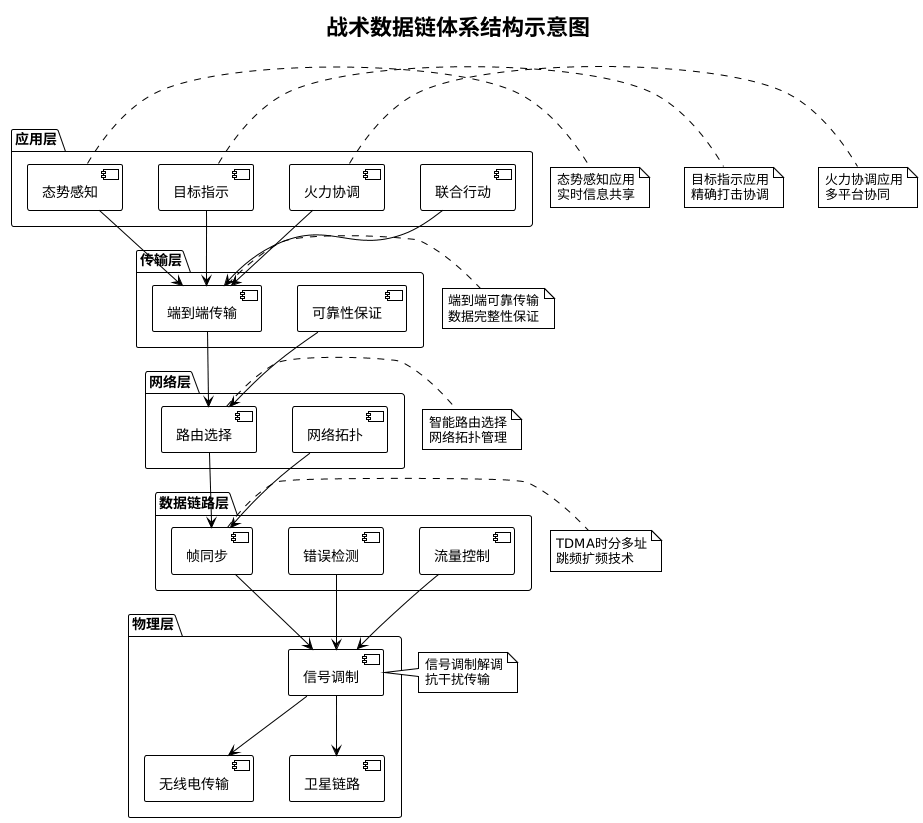
\includegraphics[width=0.8\textwidth,height=0.5\textheight,keepaspectratio]{chapters/fig-0/tdl_architecture_simple.png}
    \caption{战术数据链体系结构示意图}
    \label{fig_tdl_architecture}
\end{figure}

而在北约、美军体系内部,{Link16} 因其具有高速率,抗干扰、加密等特点,被大规模部署到空、海、地等各种平台之中\cite{Ultra_ADSI_2023},被用态势感知、目标标示、火力协同、联合任务等。但随着多链并存、跨域作战等要求的出现,这些原有链路也开始暴露出互操作困难、利用率有限等问题。

Link16的先进性主要体现在其TDMA接入和跳频扩频技术上。TDMA技术是指利用时分多址,多个平台同时工作在同一频段,互不干扰,提高频谱使用效率。Link16跳频扩频技术是指通过快速跳频抗干扰和抗截获,以提高系统的抗干扰性和安全性。Link16采用加密算法对数据进行加密,例如:KGV-8加密机对传输的信息进行加密。

在应用层方面,Link16载荷着各类J系列消息,包括J2.0(基干入网)、J3.0(航迹管理)、J3.2(空中航迹)、J3.3(水面航迹)、J3.5(空中航迹扩展)、J7.0(任务管理)、J12.0(电子战)等。这些消息涵盖着现在作战的方方面面,从简单的航迹消息到复杂的任务协调,为多平台之间的协同作战提供了完整的信息基础。

然而,由于作战的复杂性和作战需求的多样性,Link16也面临着一些挑战。首先是带宽限制问题,虽然 Link16 的传输速率已经较早期系统有很大提高,但是面对大量高清图片、视频等数据的处理能力仍有所欠缺。其次是互操作性问题,不同国家和厂商的设备可能在实现 Link16 标准上存在细微差别,这降低了系统的互操作性。最后是网络安全问题,随着网络攻击手段的不断演进,可能对传统的加密和认证方案形成挑战。

针对这些问题,各个国家国防部队和工业部门均研制有新一代的战术数据链技术,保留Link16优势的前提下,增加带宽、网络安全和与现有技术的兼容性,同时人工智能、机器学习等技术也在一定程度上助力战术数据链技术的智能化进程。

\section{MIL-STD-6016 标准框架与特点}
MIL-STD-6016 作为 {Link16} 的核心标准,对 J 系列报文的格式、语义及应用场景做出了详细规定\cite{ASSIST_6016_2024,CJCSM_6235_01_2025}。其主要特点包括:  

(1)统一的 J 系列消息目录,覆盖作战控制、目标指示与火力支援等功能;  

(2)采用时分多址(TDMA)机制,保证在高密度网络中的有序通信;  

(3)抗干扰能力强,结合跳频扩频和加密算法,提升系统的安全性和鲁棒性;  

(4)具备扩展性,可通过 {JREAP} 协议实现超视距(BLOS)传输,并与 {TTNT} 等新型战术网络互操作。

此外,MIL-STD-6020 明确了跨数据链数据转发与映射的规则;NATO 的 STANAG 5602 及其配套 SIMPLE 规范为异构链路互连提供了标准化接口;而 SISO 标准给出了 {Link16} 仿真的数据模型与交互定义\cite{Ultra_MDLMS_2021}。这些标准共同构成了战术数据链互操作的规范框架。

MIL-STD-6016标准的确立是美军多年来相关战术数据链标准化工作的结果。此标准规定了消息结构、消息语义、J系列消息,并定义了消息处理流程、消息处理错误。每一个消息类型都有明确定义,消息结构、每个字段含义、取值、处理规则等,都为厂商实现设备提供了标准。

图\ref{fig_j_series_message_structure}给出了 MIL-STD-6016 中 J 系列消息的总体框架,展示了消息的分类和组织结构。图中,将 J 系列消息分为六大类:作战控制类(J0-J9)、电子战类(J10-J19)、情报类(J20-J29)和武器协调类(J30-J39),每类消息都有其特定的应用场景和功能定位,体现了标准设计的系统性和完整性。

\begin{figure}[H]
    \centering
    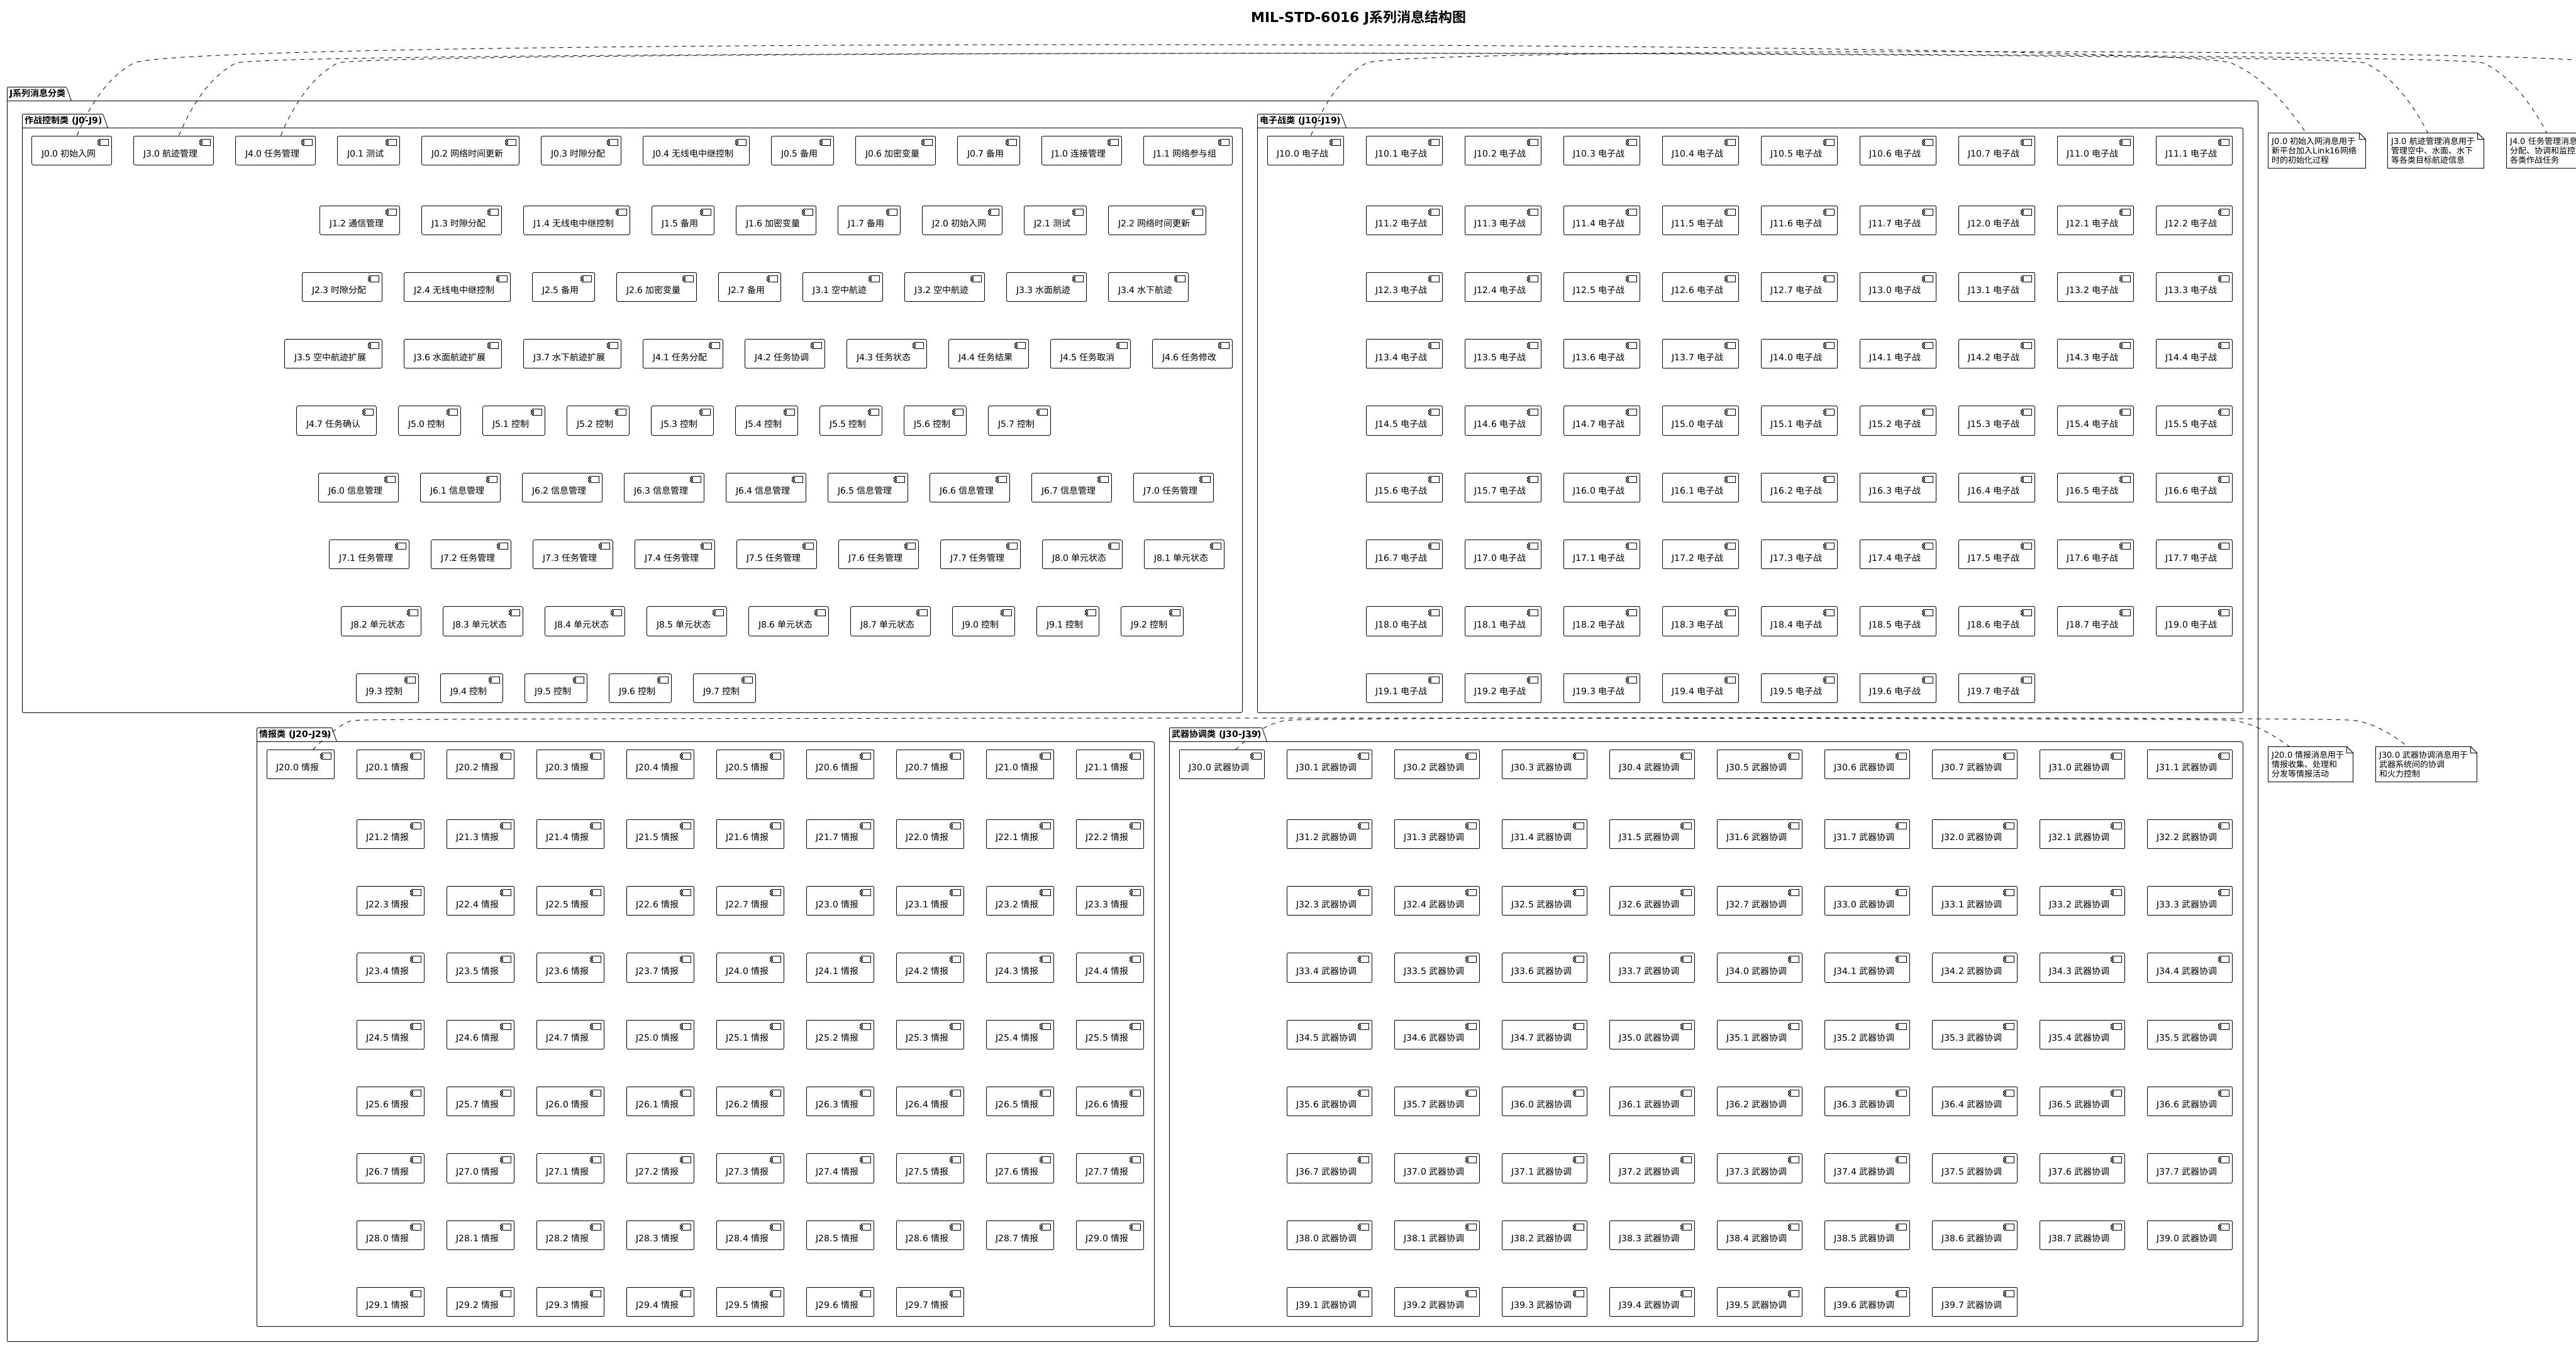
\includegraphics[width=0.85\textwidth,height=0.6\textheight,keepaspectratio]{chapters/fig-0/j_series_message_structure.png}
    \caption{MIL-STD-6016 J系列消息结构图}
    \label{fig_j_series_message_structure}
\end{figure}

在消息格式方面,MIL-STD-6016设计了固定长度消息与可变长度消息,其中固定长度消息处理简单且传输速度快,适合一些实时性要求高的应用,可变长度消息适合于复杂程度不同的消息传输需求,提高了系统的灵活性。这种设计使得Link 16能够同时支持简单的状态报告和复杂的任务协调信息。

标准同时对于消息的语义一致性问题也给予了关注,由于战术数据链涉及到了多军种、多国家平台,消息语义的一致性是互操作能否实现的关键点,在MIL-STD-6016中消息语义一致性的问题通过数据字典、语义规则等的定义使得在不同平台之间信息交互时,对交换信息拥有一致的解析。

随着技术的进步,MIL-STD-6016标准也在不断地发展完善,新版标准在原有基础上扩充了新的消息类型,对原有的一些格式也进行了升级,使其适应新的作战需求和技术发展;此外,增加了网络安全和抗干扰能力,反映了新的作战环境对通信系统安全性的需求。

在标准实施上,美军的各兵种以及工业企业都投入了大量资源来保证标准化的互操作性,包括建立标准化试验、认证、兼容性试验程序来保证MIL-STD-6016在世界范围内的良好实施,为多国联合作战提供技术保障。

表\ref{table_mil_std_comparison}中给出了MIL-STD-6016标准与其他标准的优缺点和应用范围以及互操作能力。在表中可以很清楚的看出MIL-STD-6016标准作为Link16中的核心标准,在消息结构方面、消息传递方面以及互操作性方面都有着独特的优势,是实现战术数据链标准化技术的基础,为战术数据链的互操作提供了一定的技术支持。

\begin{table}[H]
    \caption{MIL-STD-6016相关标准对比分析表}
    \label{table_mil_std_comparison}
    \centering
    \adjustbox{width=0.95\textwidth,center}{%
    \begin{tabular}{lcccc}
        \toprule
        \textbf{标准名称} & \textbf{主要功能} & \textbf{应用范围} & \textbf{互操作性} & \textbf{技术特点} \\
        \midrule
        MIL-STD-6016 & J系列消息格式定义 & Link16战术数据链 & 强 & TDMA、跳频扩频、加密 \\
        & 消息语义规范 & 联合作战平台 & & 固定/可变长度消息 \\
        & 处理流程标准 & 多军种协同 & & 实时性、可靠性 \\
        \midrule
        MIL-STD-6020 & 跨数据链转发 & 多链路互连 & 中等 & 数据映射、格式转换 \\
        & 数据映射规则 & 异构系统集成 & & 协议适配、路由选择 \\
        & 互操作接口 & 联盟作战 & & 标准化接口 \\
        \midrule
        STANAG 5602 & NATO互操作标准 & NATO成员国 & 强 & 统一数据格式 \\
        & SIMPLE规范 & 联盟协同作战 & & 标准化接口 \\
        & 异构链路互连 & 多国联合作战 & & 兼容性保证 \\
        \midrule
        SISO标准 & 仿真数据模型 & Link16仿真系统 & 中等 & 仿真接口标准 \\
        & 交互定义 & 训练与测试 & & 数据模型规范 \\
        & 仿真互操作 & 系统验证 & & 标准化仿真 \\
        \bottomrule
    \end{tabular}%
    }
\end{table}

\section{微服务架构}

微服务架构(Microservice Architecture, MSA)是当今软件工程的最新发展趋势之一,微服务概念的基本思想在2010年前后已经有相关文献提出,James Lewis和Martin Fowler在2014年提出了微服务的概念,是一种以业务能力为中心的模块化架构,具有服务自治、低耦合、可自部署的显著特征,与传统应用程序相比,微服务具有独特的持续交付灵活迅速且可独立模块的能力。2015年,被称为“微服务元年”,Netflix、Amazon、Google等在大规模分布式系统中引入微服务模型,部署服务注册中心、API网关、容错机制,实现服务治理、弹性伸缩、高可用部署,标志着微服务从企业实践逐步走向“学术研究深水区”。

2018-2020年国外学者将研究的重点放在微服务系统的研究及评价上,Waseem\cite{Waseem2021Design}等人基于106份调查问卷和其他调查,对微服务系统的设计、监视和测试做出了总结。他们认为领域驱动的设计(DDD)和基于业务能力服务拆分是目前应用最广泛的设计方式,API网关和Back-end架构是最常用的架构,而资源利用率、负载均衡和日志聚合作为监视的关键领域,微服务工程中模块难以明确、边界划分和自动化测试是普遍存在的问题。此阶段的研究为微服务架构中的质量属性、监视和测试提供了经验,为进一步的研究铺平了道路。

分布式数据系统与云原生技术的发展也为微服务研究注入了新的动力。Laigner等在《Data Management in Microservices》中分析了30多个工业案例和论文,认为Database Per Service模式能够解决跨服务问题和跨服务数据问题,但也会带来数据一致性新问题,需要结合跨服务数据库和Saga模型、事件和最终一致模式来确保可靠性和性能\cite{Laigner2021Data}。后续研究进一步提出面向微服务的基准测试体系,如《Benchmarking Data Management Systems for Microservices》与《Online Marketplace》两篇工作,从事务处理、事件一致性与数据复制角度评估数据管理系统性能,为微服务数据库化演进提供了实验标准 \cite{BenchmarkingDataMgmt2024,OnlineMarketplace2024}。与此同时,Giamattei 等人开展了针对 71 种微服务监控工具的系统性灰文献回顾,总结出资源监控、日志追踪与可观测性平台的实践经验,揭示出当前工具生态存在指标标准不统一与跨层数据整合不足的问题 \cite{MonitoringTools2023}。

安全方面,由于微服务系统的复杂性,也存在基于微服务的访问控制、认证方面的工作。部分工作提出微服务的“零信任”模型,通过轻量级认证(OAuthentication2.0,JWT)和服务网格实现微服务间的安全通信,实现流量分割和细粒度授权。这些工作也进一步促进了未来的 DevSec Operations 和安全问题自动化,国外的学术工作已经关注到了微服务架构的智能和自适应机制设计,通过 AI 和机器学习技术来实现微服务部署调度优化、容器调度、异常发现自动化等,将微服务系统变为动态自适应系统。

国内的微服务研究应用在2010年前后肇始,2007年,阿里巴巴淘宝应用分布式服务框架,开启国内微服务化进程,国内涌现出Dubbo、Spring Cloud阿里巴巴、ServiceComb等一批国产开源框架,企业级系统微服务化应用得到极大发展。2020年前后,国内学者和军工科研机构开始探索复杂信息系统微服务,引入战术通信、指挥控制平台,研究内容主要是服务拆分、容器化、服务编排、跨节点一致控制。一些科研机构开始将微服务集群应用于态势信息处理平台和模拟平台,实现任务模块独立运行和微服务弹性伸缩。国内研究从框架复用和工程应用转向框架设计和性能实验、面向军事通信系统应用的微系统构型开始形成。

图\ref{fig_microservices_evolution_timeline}给出了微服务架构的演进时间轴,从技术理论阶段到智能发展阶段过程清晰,从时间纬度,展示了国外2010年到2014年的概念、理论,2015年到2017年的企业实践、云原生和2018年到2020年的系统研究、2021年至今的智能发展阶段,体现微服务技术的成熟和应用深入。

\begin{figure}[H]
    \centering
    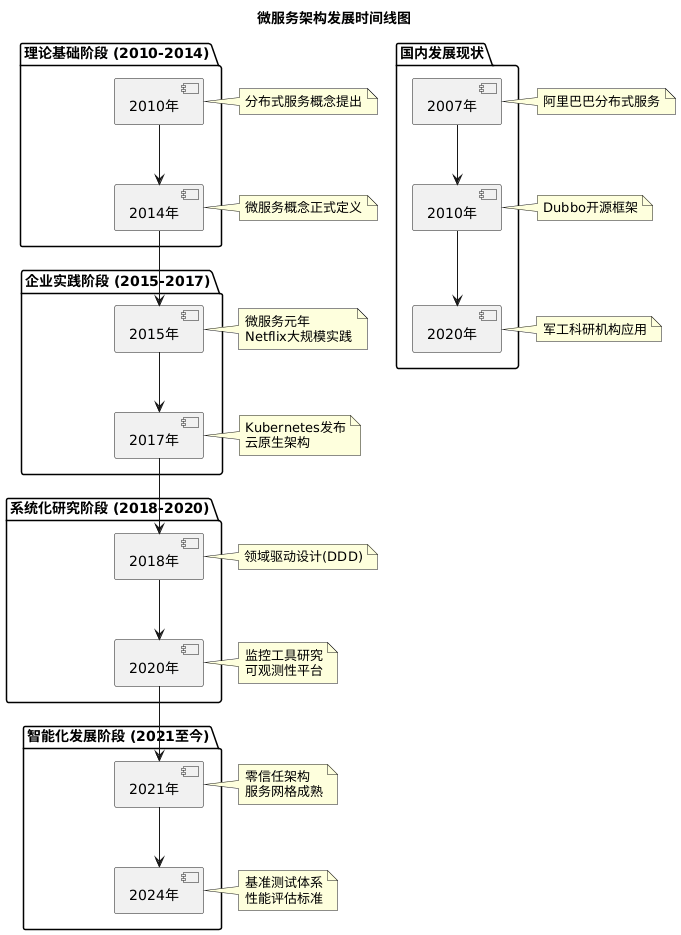
\includegraphics[width=0.8\textwidth,height=0.6\textheight,keepaspectratio]{chapters/fig-0/microservices_evolution_timeline.png}
    \caption{微服务架构发展时间线图}
    \label{fig_microservices_evolution_timeline}
\end{figure}


\section{语义互操作}

语义互操作(Semantic Interoperability)是异构系统在数据交换过程中实现“语义层理解一致”的关键能力,其核心目标是让信息在不同系统、组织或领域间传输时,不仅保持结构一致,还能被准确解释和复用。该概念最早起源于语义网与本体论研究,通过形式化语义模型描述数据背后的概念及其关系,为复杂系统间的理解一致提供理论基础。随着信息系统复杂性与数据异构性的增加,语义互操作逐渐成为人工智能、云计算、医疗健康、工业物联网等领域的核心研究方向。

在国际研究领域,早期的语义互操作工作侧重于标准体系的构建与模型分层。SISO、NATO和ISO等多层互操作模型的提出,将信息互操作划分为语法、语义、语用层\cite{SISO_STD_002_2006,CJCSI_6610_01F_2021},为后续研究提供了一个参考统一体模型。2010年以后,部分学者开始对本体(Ontology)[25]在语义互操作中的应用进行研究。Mishra和Jain提出了“语义知识宝库”(Semantic knowledge treasure),通过OWL和SPARQL完成异构资源统一语义表示和查询\cite{Mishra2018Semantic}。这些研究,标志着语义互操作由概念层面进入知识层面。

近几年,在知识图谱、自动推理、人工智能等技术的推动下,语义互操作研究向智能、自动方向研究。Bernasconi等提出“本体解包”(Ontological Un-packing)方法对已有概念模型进行本体分析,揭示概念模型隐性语义结构,提高模型互操作性\cite{Guizzardi2023Explanation}。Guizzardi 与 Guarino 则在《Semantics, Ontology and Explanation》中引入语义互操作诠释问题,即语义透明性和本体承诺(Ontological Commitment)应作为提高互操作和可理解性和可信赖性的手段\cite{Guizzardi2023Explanation}。此外,机器学习与规则引擎结合的语义映射算法自动获取概念映射关系,进行跨领域知识语义对齐和重用。

随着云与分布式系统应用越来越广泛,语义互操作也扩展到跨平台和多云场景。Hamdan和Admodisastro提出了一种基于本体层(metalayer)的多云语义互操作参考模型,并在参考模型基础上设计了语义中心(Semantic Hub)用来协调不同云场景中的语义模型,并提供语义一致性服务\cite{Hamdan2023Reference,SemanticMultiCloud2024}。同时指出,在异构场景中保持语义一致性需要在三个模型层进行协同,即架构层、数据层和治理层;同时语义互操作也在与数据治理、知识发现、可解释人工智能等研究进行深度融合,为跨平台和协同提供基础能力。

国内语义互操作研究源于 2000 年代的语义网工程,近年来知识图谱和人工智能的兴起,进一步推动了语义互操作研究。语义本体构建、语义映射方法、语义信息检索、语义推理机制等研究热度持续攀升。以知识图谱为研究对象,在构建语义关系模型的基础上,对异构数据进行实体映射、语义标注,从而实现可融合性;以智慧城市、医疗、交通、工业互联网应用为研究对象,以语义互操作为核心,研究多源数据融合与协同管理。语义互操作研究从“语义建模”转向“语义计算”的研究,以语义理解、语义推理和动态本体演化为核心,满足即时性、可解释性强的新需求。

语义互操作体系结构层次从物理层到语用层共分为4层架构模式。具体语义互操作系统体系结构的层次如\ref{fig_semantic_interop_architecture}所示,物理层实现传输协议和网络互联,语法层实现数据格式、消息结构,语义层实现本体模型和概念映射,语用层实现业务规则、上下文理解等,互操作机制中的语义中枢、映射引擎、转换器、验证器体现了语义互操作技术的抽象和完整性。

\begin{figure}[H]
    \centering
    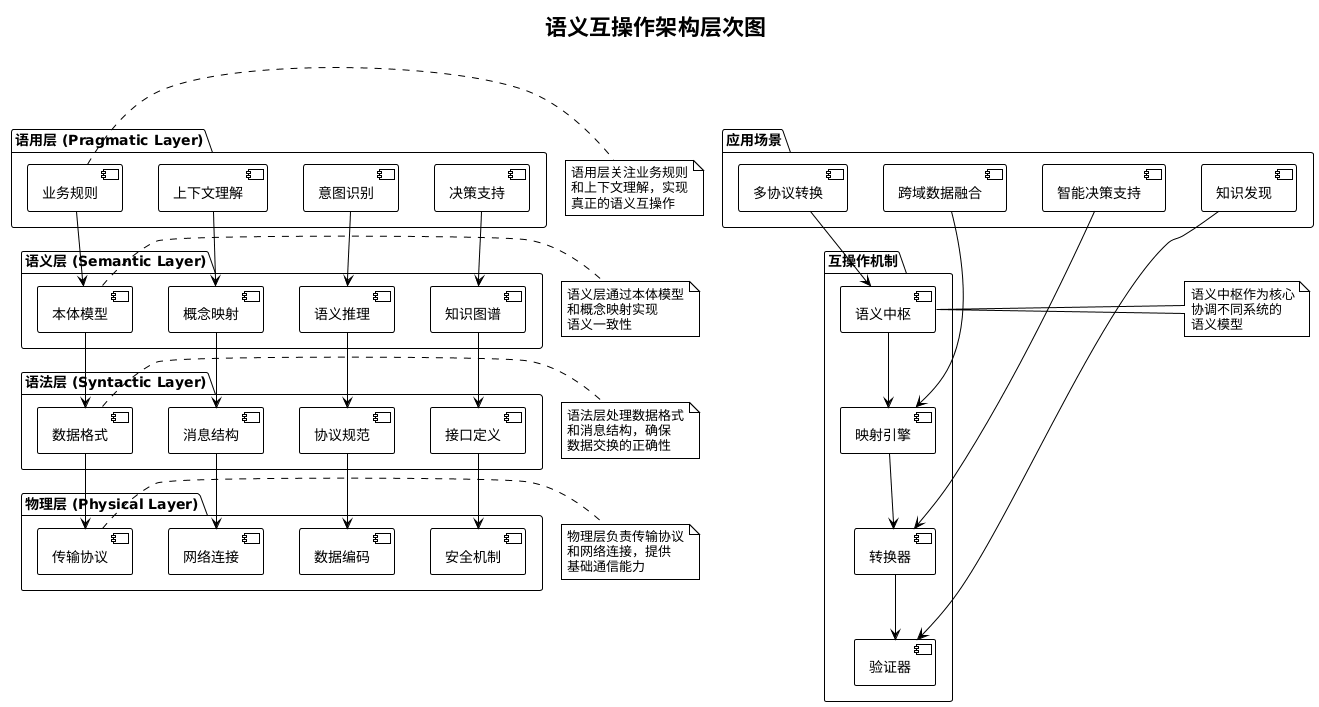
\includegraphics[width=0.85\textwidth,height=0.7\textheight,keepaspectratio]{chapters/fig-0/semantic_interop_architecture.png}
    \caption{语义互操作架构层次图}
    \label{fig_semantic_interop_architecture}
\end{figure}


\section{自动化处理}

自动化处理技术是复杂信息系统中的必要技术,主要是为了将非结构化(半结构化)文档(PDF、Word、XML、JSON等文件)进行自动解析、识别、导入数据库或其他知识系统中进行高效、精准的建模和信息抽取,经过了基于规则的处理到机器学习、深度学习等智能处理的发展历程,近年来,在自然语言处理、智能文档处理(Document Intelligence)、多模态学习等方面取得了快速发展。

早期的自动化文档处理研究以版面分析(Layout Analysis)和文本块识别为主要方法。典型工作包括基于光学字符识别(OCR)的文本抽取、表格检测与区域定位算法。这一阶段的研究主要依赖启发式规则与图像分割算法,如 PDFMiner、Apache Tika 等工具框架,通过对文本流与版面结构的分析实现基本的内容解析。然而,这些方法难以处理复杂文档中的语义结构与跨页逻辑关系。

随着深度学习和自然语言识别的发展,更多基于网络的文档识别和语义理解模型被提出。2020年起,Google、Microsoft、Adobe等机构使用视觉语言联合模型(Vision-language Models)进行文档识别和文档阅读任务\cite{Xu2020LayoutLM,Xu2022LayoutLMv3},Xu等使用联合模型对文本、位置和视觉信息进行建模,对文档结构和语义进行理解和识别,如表单识别、关键字识别、文档分类等。论文中的基于Tensor多模态的方法在识别PDF结构时获得了不错的效果。该方法为复杂结构文档识别提供了一个通用的框架。

在信息抽取与结构化导入方向,学者们提出了多种智能抽取与标准映射框架。Li 等在《DocParser: Document Parsing and Structured Data Import》\cite{Li2021DocParser} 中提出一种结合文本分块、实体识别与模板匹配的自动导入机制,实现 PDF 与 XML 文档的语义级结构化导入。与此同时,研究者将知识图谱构建与自动文档处理相结合,通过实体识别、关系抽取与语义对齐实现从原始文档到知识图谱的自动生成,为数据标准化与语义互操作奠定了基础。此类方法已在专利文档、医学报告与技术标准文件的自动建模中得到验证。

近年来,自动化加工逐渐发展到自动化的监督学习和跨模态理解,模型不再需要人工标注而是采用海量的通用特征预训练而成,例如Powalski等人提出的文档自动分类与提取表格任务中的文本-视觉双流Transformer模型\cite{Powalski2021DocFormer}。随后,将大规模语言模型(LLM)与文档知识关联起来的跨模态语义推理与任务自适应成为研究热点\cite{Wang2023DocumentLLM},文档自动化迎来了“语义理解为王”的新时代。

国内对于自动化文档处理的研究集中于结构化识别和智能导入系统的工程化运用,研究院所及科技企业进行了对于PDF解析、表格抽取、标注字段、标准导入的研究,开发基于深度学习的OCR引擎、语义分层引擎,百度文心、阿里达摩院、华为诺亚方舟实验室等都提出了面向企业文档及技术标准的多种模态解析思路,并部分运用到企业电子政务、科研档案、装备资料中。然而,国内研究仍具有跨格式迁移能力差、语义抽象层次低、自动验证及纠错能力不足的问题,在知识表示、语义约束及可解释性方面需进一步加强。

图\ref{fig_document_processing_evolution}描述了文档的自动处理技术演化轨迹,描绘了规则驱动、机器学习、深度学习等4个阶段。从技术维度勾勒了文档自动处理技术的4个发展演进轨迹,从2000-2010年的启发式算法的规则驱动阶段,到2010-2020年的视觉语言融合模型阶段,再到2020-2023年的深度学习的Tensor架构阶段,以及2023年以来的文档自动处理技术智能化阶段,涉及电子政务、科研档案、装备资料、技术标准等各个领域。

\begin{figure}[H]
    \centering
    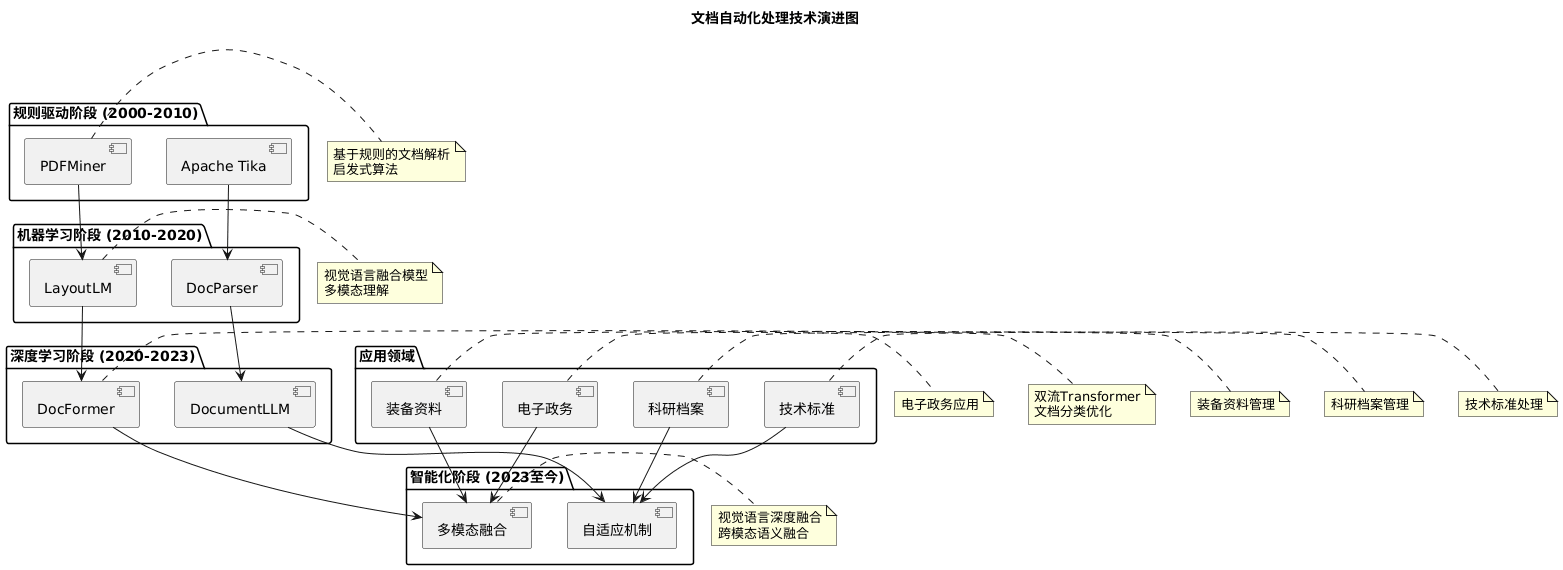
\includegraphics[width=0.8\textwidth,height=0.6\textheight,keepaspectratio]{chapters/fig-0/document_processing_evolution.png}
    \caption{文档自动化处理技术演进图}
    \label{fig_document_processing_evolution}
\end{figure}

\section{本章小结}

基于以上分析,本章系统梳理了战术数据链技术、微服务架构和语义互操作三个核心技术领域的理论基础、发展现状和技术特点。通过深入分析相关技术的研究进展和应用实践,为构建基于MIL-STD-6016标准的战术数据链信息标准数据库系统提供了坚实的理论基础。

在战术数据链技术方面,MIL-STD-6016标准为J系列消息的格式化和语义化提供了统一规范,为系统设计提供了标准依据。在微服务架构方面,其分布式、模块化的设计理念为构建高性能、高可用的数据库系统提供了技术支撑。在语义互操作方面,基于本体的语义映射机制为实现跨标准的数据融合和互操作提供了关键技术路径。

基于以上技术分析,本研究将采用微服务架构构建战术数据链信息标准数据库系统,通过语义互操作技术实现MIL-STD-6016消息的标准化存储、语义化处理和跨标准互操作,为多链融合提供统一的信息支撑平台。下一章将详细阐述系统的总体架构设计和核心算法研究。


% \cleardoublepage
\chapter{系统需求分析}

本章主要围绕基于 MIL-STD-6016 的战术数据链信息标准数据库及其应用平台,分析系统的整体需求,明确功能性与非功能性要求,以便为后续系统设计与实现提供依据。

战术数据链作为现代联合作战的核心通信手段,其信息标准数据库的建设对于提升作战效能、增强系统互操作性具有重要意义。随着网络中心战概念的深入发展和多域作战需求的不断增长,传统的战术数据链系统面临着数据管理复杂、标准版本多样、跨链路互操作困难等挑战。因此,构建一个统一、高效、可扩展的战术数据链信息标准数据库系统,已成为当前军事信息化建设的重要任务。

本章将从系统需求分析的角度,全面阐述基于MIL-STD-6016标准的战术数据链信息标准数据库系统的功能需求、非功能性需求、数据特征与处理需求以及用户角色与交互需求。通过对这些需求的深入分析,为后续的系统架构设计、数据库建模、前后端开发以及系统集成测试提供明确的技术指导和约束条件。

\section{功能需求}

根据前期调研和标准分析,结合实际应用场景,系统需要实现以下核心功能:

\subsection{数据特征与处理需求}
战术数据链消息具有与传统业务数据不同的特性,其处理需求也更为复杂。为保证数据库的适用性与系统的实用性,需从数据来源、结构特征、处理方式与存储管理等角度加以分析\cite{baek2016_jsac}。

系统数据主要来源于 {MIL-STD-6016}、{MIL-STD-3011}、{STANAG-5516} 等标准文档,并结合 {MAVLink}、{NMEA-0183}、{ARINC-429} 等协议数据。数据类型主要包括:

(1)标准消息数据:J 系列报文(J2.0、J3.0、J7.0、J12.0等)及其字段定义;

(2)语义概念数据:基于CDM四层法的概念库和字段映射关系;

(3)多格式文档数据:PDF、XML、JSON、CSV等格式的标准文档和配置文件;

(4)跨协议转换数据:不同协议间的消息转换和映射规则。

表\ref{table_data_features}详细展示了战术数据链数据特征与处理需求的对应关系,该表从数据类型、结构特点、处理需求和存储实体四个维度进行了系统性的分析。

\begin{table}[!htb]
    \caption{战术数据链数据特征与处理需求概览}
    \label{table_data_features}
    \centering
    \adjustbox{width=0.9\textwidth,center}{%
    \begin{tabular}{lccc}
        \hline
        \textbf{数据类型} & \textbf{结构特点} & \textbf{处理需求} & \textbf{存储实体} \\
        \hline
        标准消息数据 & 多字段/比特位 & 报文解析、完整性校验 & 消息表、字段表 \\
        语义概念数据 & 概念层次/同义映射 & 概念绑定、语义一致性 & 概念表、绑定表 \\
        多格式文档数据 & 格式多样/结构复杂 & 多格式解析、智能识别 & 文档表、解析结果表 \\
        跨协议转换数据 & 格式差异/协议适配 & 格式转换、协议映射 & 映射表、转换规则表 \\
        \hline
    \end{tabular}%
    }
\end{table}


\subsection{标准消息管理}
战术数据链信息标准数据库系统需要支持多种消息标准的统一管理\cite{CurtissWright_TCG_HUNTR_2020}。根据实际应用需求分析,系统应具备以下核心能力:

(1)多标准消息支持:系统需要同时支持MIL-STD-6016的J系列消息(J2.0、J3.0、J7.0、J12.0等)、MAVLink的飞行器通信消息(HEARTBEAT、ATTITUDE、POSITION等)、NMEA-0183的导航消息(GGA、RMC、VTG等)等多种标准。每种消息标准都有其特定的格式、语义和应用场景,系统需要能够完整地存储和管理这些消息的定义信息,包括消息的基本属性、消息结构以及消息的语义信息。

下表\ref{table_supported_standards}详细列出了系统需要支持的主要标准和协议。

\begin{table}[!htb]
    \caption{系统支持的标准和协议}
    \label{table_supported_standards}
    \centering
    \adjustbox{width=0.9\textwidth,center}{%
    \begin{tabular}{lccc}
        \hline
        \textbf{标准名称} & \textbf{描述} & \textbf{版本} & \textbf{主要消息类型} \\
        \hline
        MIL-STD-6016 & 美军标准6016 - 战术数据链消息标准 & A, B, C & J2.0, J3.0, J7.0, J12.0, J13.0 \\
        MIL-STD-3011 & 美军标准3011 - 联合战术信息分发系统 & A, B & J2.0, J2.2, J3.0, J3.1, J3.3 \\
        STANAG-5516 & 北约标准5516 - 战术数据交换 & 1, 2, 3 & J2.0, J3.0, J7.0, J12.0 \\
        MAVLink & 微型飞行器通信协议 & 1.0, 2.0 & HEARTBEAT, ATTITUDE, POSITION, GPS\_RAW\_INT \\
        NMEA-0183 & 海洋电子设备数据格式 & 2.0, 2.1, 2.2, 2.3 & GGA, RMC, VTG, GLL, GSA \\
        ARINC-429 & 航空电子设备数字信息传输 & 15, 16, 17 & A429, A629 \\
        \hline
    \end{tabular}%
    }
\end{table}

(2)消息录入与维护:考虑到标准文档的复杂性和多样性,系统需要支持多种数据录入方式。传统的逐条录入方式效率低下,无法满足大规模标准文档的处理需求。系统需要提供基于PDF文档的自动化解析功能,能够从标准文档中自动提取消息定义信息,并支持CSV、Excel、XML、JSON等多种格式的批量导入和单个录入两种方式。

(3)消息字段管理:J系列消息的字段结构复杂,包含字段名称、起始位置、结束位置、位长度、描述信息等多个属性。系统需要能够处理这种复杂的字段结构,并建立字段与消息之间的关联关系。同时,系统需要支持字段的层次化组织,如字段组、子字段等,以便于更好地管理和理解消息结构。


\subsection{字段与语义概念绑定}
为提升消息语义一致性,系统需要支持字段与语义概念的绑定\cite{Chelton_Link16_Antennas_2022}。根据实际应用需求分析,系统应具备以下核心能力:

(1)语义概念库构建:需建立统一的语义概念库,包含战术数据链领域中的核心概念,如平台标识、位置信息、时间信息、任务状态等。每个语义概念都应具有明确的定义、属性描述和使用规则,支持概念的层次化组织和继承关系。

(2)字段绑定机制:系统需要支持自动绑定和手动绑定两种方式。自动绑定基于字段名称、数据类型、取值范围等特征进行匹配,能够快速建立初步的绑定关系。手动绑定允许专家用户根据领域知识进行精确的绑定操作,确保绑定的准确性和完整性。

(3)置信度管理:在功能上需要为每个字段-概念绑定关系分配置信度值,反映绑定的可靠程度。置信度可以通过字段名称相似度、数据类型匹配度、专家验证结果等因素计算,并提供置信度阈值设置功能,允许用户根据应用需求调整绑定标准。

(4)动态绑定更新:考虑到战术数据链标准的不断演进,应支持语义绑定的动态更新,当标准版本更新或新增消息类型时,能够自动检测需要重新绑定的字段,并提供批量更新功能。

\subsection{多链路互操作支持}
考虑到战术数据链存在多标准并行的情况,系统需要具备跨链路的互操作支持功能\cite{AFCEA_Link16_Improvements_2022}。根据实际应用需求分析,系统应具备以下核心能力:

(1)CDM四层法架构:系统需采用CDM(Common Data Model)四层法架构实现多协议互操作。概念层定义统一的语义概念库,包含作战实体、态势要素、指挥关系等核心概念;映射层通过声明式规则定义协议间的字段映射关系;转换层实现具体的消息转换逻辑;运行层提供协议中介和转换引擎。系统支持MIL-STD-6016、MAVLink、MQTT、NMEA-0183等协议的互操作转换,这种分层架构确保系统的可扩展性和可维护性。

图\ref{fig_cdm_architecture}展示了CDM四层法架构,包括语义层(统一概念库)、映射层(YAML配置规则)、校验层(一致性验证)和运行层(转换引擎),展现了多协议间的语义互操作和实时转换。

\begin{figure}[H]
    \centering
    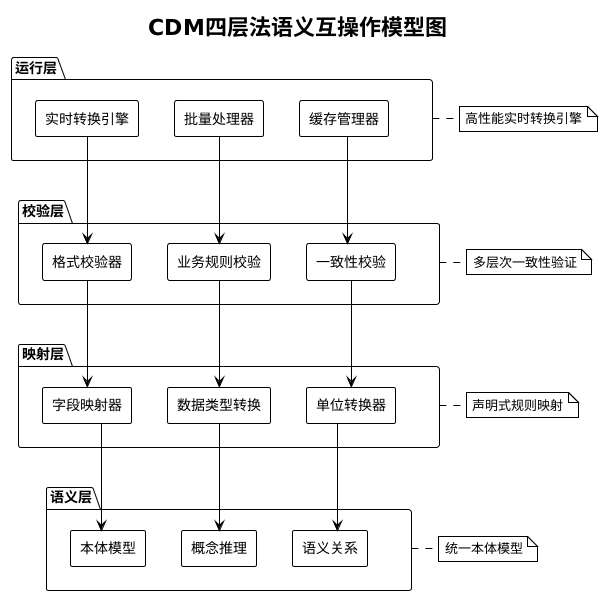
\includegraphics[width=0.6\textwidth,height=0.5\textheight,keepaspectratio]{chapters/fig-0/cdm_four_layer_simple.png}
    \caption{CDM四层法架构图}
    \label{fig_cdm_architecture}
\end{figure}

(2)智能消息转换引擎:应实现基于规则和机器学习的智能转换引擎,能够自动处理协议间的语法差异、语义差异和时序差异。转换引擎需要支持多种转换策略,包括精确匹配、模糊匹配、语义推理等,并提供转换质量评估和置信度评分机制。

(3)统一API网关:需提供统一的API网关,支持多种协议的消息转换和路由。网关需要集成CDM四层法和语义互操作两种处理方式,能够根据源协议和目标协议自动选择最优的转换策略。
下表\ref{table_api_interfaces}列出了系统提供的5个主要API接口及其功能,通过RESTful架构设计为前端界面和外部系统提供标准化数据交换接口。

\begin{table}[!htb]
    \caption{系统API接口功能表}
    \label{table_api_interfaces}
    \centering
    \adjustbox{width=0.9\textwidth,center}{%
    \begin{tabular}{lccc}
        \hline
        \textbf{API接口} & \textbf{主要功能} & \textbf{支持格式} & \textbf{应用场景} \\
        \hline
        /api/v2 & 消息转换、概念管理、映射管理、系统统计 & JSON, XML & 统一文档处理与语义互操作 \\
        /api/cdm & CDM概念创建、映射规则管理、消息转换 & JSON, YAML & CDM四层法互操作处理 \\
        /api/semantic & 语义字段管理、消息映射、路由处理 & JSON, XML & 语义互操作系统 \\
        /api/pdf & PDF文档解析、表格提取、数据处理 & PDF, JSON & MIL-STD-6016文档处理 \\
        /api/mqtt & MQTT消息处理、协议转换、数据路由 & JSON, MQTT & MQTT协议消息处理 \\
        \hline
    \end{tabular}%
    }
\end{table}

(4)协议适配支持:功能设计上应支持MIL-STD-6016、MAVLink、MQTT、NMEA-0183、ARINC-429等多种协议的消息对接,能够处理不同协议间的消息格式差异、语义差异和时序差异。通过声明式映射规则和版本治理机制,系统需要能够灵活应对协议演进和标准更新。


\subsection{前端交互与可视化}
基于前述数据库操作与维护的需求,战术数据链信息标准数据库系统面向的用户群体包括系统管理员、作战指挥员、研发人员等,这些用户具有不同的技术背景和使用需求,因此前端系统应具备以下核心能力:

(1)统一用户界面:需提供统一文档处理与语义互操作平台,包含消息处理、文件处理、概念管理、映射管理、系统概览等核心功能模块,支持用户通过消息号、字段名、J系列类别、时间范围等多种条件进行精确查询,并支持查询条件的保存和重用,允许用户创建常用的查询模板。

(2)数据展示与搜索:应支持多种数据展示方式,包括表格、图表、关系图等,其中表格展示需支持排序、筛选、分页等功能,并提供数据导出能力,图表展示应支持多种图表类型,如柱状图、饼图、折线图等,帮助用户直观地理解数据分布和趋势。同时,系统还应提供智能搜索功能,支持模糊匹配和语义搜索,帮助用户快速定位所需信息。

(3)交互式操作:为确保良好的用户体验和系统可用性,需支持交互式操作和响应式设计。系统应支持拖拽、点击、缩放等交互操作,允许用户通过直观的手势操作来浏览和操作数据,并提供上下文菜单、快捷键等便捷操作方式,提高用户的操作效率。

系统需针对不同用户提供差异化的交互模式\cite{reid_2018_nav_leo}:

(1)图形化交互:前端界面提供消息检索、态势展示和跨链协议映射的可视化操作,支持CDM互操作接口、语义互操作接口和统一处理器接口,降低使用门槛,如图\ref{fig_usecase_frontend}所示。
% ================= 新增:用例图 =================
\begin{figure}[H]
    \centering
    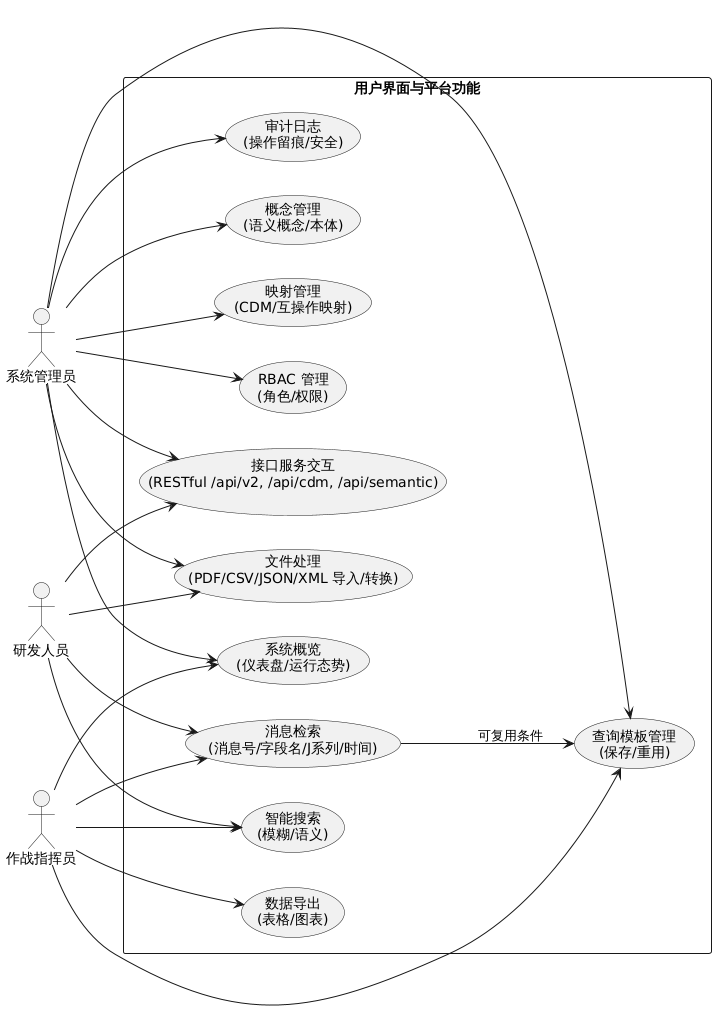
\includegraphics[width=0.8\textwidth,height=0.5\textheight,keepaspectratio]{chapters/fig-0/usecase_frontend.png}
    \caption{前端交互用例图(角色与功能关系)}
    \label{fig_usecase_frontend}
  \end{figure}
(2)命令行接口:为研发与仿真人员提供批处理与脚本化调用,支持大规模数据处理与自动化测试。

(3)接口服务交互:通过 RESTful API 与外部仿真平台或作战系统对接,支持标准化协议调用和跨域互操作,提供/api/v2、/api/cdm、/api/semantic等统一API接口,如图\ref{fig_component_frontend} 所示。



% ================= 新增:组件图 =================
\begin{figure}[H]
  \centering
  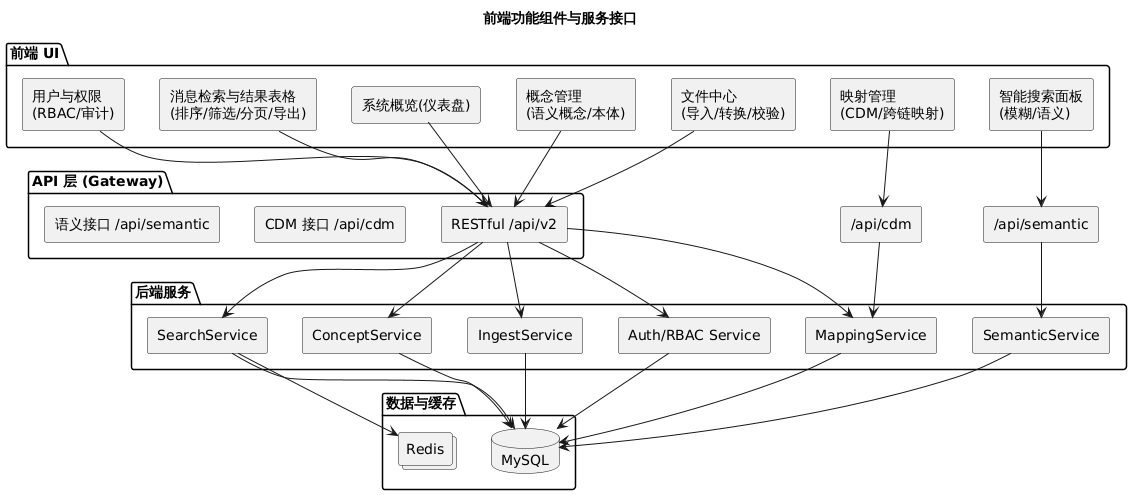
\includegraphics[width=0.8\textwidth,height=0.6\textheight,keepaspectratio]{chapters/fig-0/component_frontend.png}
  \caption{前端功能组件与服务接口关系图}
  \label{fig_component_frontend}
\end{figure}


\subsection{仿真与验证接口}
战术数据链系统的验证与测试依赖于高质量的仿真数据支撑,而仿真平台的有效运行则需要准确的消息定义和格式规范作为基础。基于这一需求,系统必须构建完善的仿真与验证接口体系。

而在面向接口设计时,系统应采用标准化的RESTful API架构,为仿真平台提供数据查询、消息生成、结果验证等核心功能。接口实现严格遵循REST架构原则,采用标准HTTP方法和状态码,确保接口的易用性和可维护性。同时,系统支持多种标准化消息输出格式(JSON、XML、YAML),满足不同仿真平台的格式需求。消息格式包含完整的定义信息,涵盖消息结构、字段定义、语义信息等关键要素,保障仿真平台对消息数据的准确理解和处理。

\section{系统非功能性需求分析}

战术数据链数据库及应用平台作为支撑作战指挥的关键信息系统,除了满足功能性需求外,还必须具备良好的非功能性特征,包括性能、安全性、可扩展性等方面的要求,以确保系统在复杂作战环境下的稳定运行和长期发展\cite{Kagioglidis_2009}。

\subsection{性能需求}
基于战术数据链系统的实时性特征和作战指挥的时效性要求,系统性能需求分析应从响应时间、数据吞吐量和系统可靠性三个维度进行考量\cite{Kee_2008,baek2016_adhoc,baek2019_jsyst_timemirror}。响应时间需求分析表明,多用户并发访问场景和实时态势更新的业务需求对系统响应性能提出了严格要求。通过分析战术数据链消息解析与字段检索的快速响应要求,可以确定普通查询请求的平均响应时间应控制在2秒以内,这一指标直接影响作战指挥的决策效率。为满足上述性能要求,系统需要实现缓存机制,包括Redis缓存和查询结果缓存,对于频繁访问的消息类型和字段定义实现预加载策略,同时建立数据库索引支持多条件组合查询的快速执行。

而对于数据吞吐量的需求,则决定了系统需要处理大规模批量数据导入导出操作,以支撑标准文档的批量处理和系统初始化需求。通过分析仿真测试场景的数据处理需求,可以确定仿真接口应具备持续处理高并发消息流的能力,实现消息的实时生成与回放功能,满足大规模仿真测试的数据处理需求\cite{lee2018_jsyst,Spyridis_2010,Kopp_Throughput_Enhanced_JTIDS_2006,Juarez_2025}。系统可靠性需求分析表明,战术环境的复杂性和不确定性对系统容错能力和数据完整性保障提出了严格要求。通过分析数据安全性和一致性要求,可以确定数据库应具备备份与日志恢复能力,确保数据在异常情况下的安全性。同时,消息存储与语义绑定过程的事务一致性约束需求进一步强化了对系统可靠性的要求,以避免数据不一致问题\cite{Koromilas_2009,EverythingRF_STT}。

\subsection{安全性需求}
战术数据链系统涉及敏感作战信息,安全性需求至关重要。系统必须在数据存储、传输与访问控制等方面提供基本的安全保障,以确保信息不被篡改、泄露或非法利用\cite{Collins_TTNT_immersion_2020}。系统应在数据存储和传输过程中采用加密技术,数据库层面应对核心字段进行加密存储,系统接口需采用基于TLS/SSL的安全传输协议,防止中间人攻击,消息交互采用密钥管理机制,定期更新密钥,防止密钥泄露\cite{Euromids_2025_contract}。

为防止非法访问与误操作,需要建立访问控制机制,提供基于角色的访问控制(RBAC),不同用户角色具备不同权限范围,对数据库的读写操作需进行身份认证与授权,提供日志审计功能,记录用户操作轨迹,便于事后追溯\cite{GovConWire_Euromids_2025}。系统应提供数据校验与完整性验证机制(如哈希校验),在通信中断或错误发生时,系统可通过重传机制与数据恢复策略保证一致性\cite{musumeci_2014_ietrsn_pulseblank,borio_2013_ietspr_pulseblanking,houdzoumis2009_jn,wu_2016_taes_dme_wp,huo_2015_ieeecl_meb,huo_2015_comex_mixed_interference,mitch_2016_nav_chirp_geolocation,vandermerwe_2023_nav_mpanf}。

\subsection{可扩展性需求}
基于战术数据链标准的不断更新与作战样式的演进趋势,系统可扩展性需求分析应从标准适配、协议融合和架构扩展三个层面进行考量\cite{CJCS_Manuals_Library}。标准适配需求分析表明,系统需要具备对不同版本Link 16标准以及相关NATO STANAG扩展的适配能力。通过分析MIL-STD-6020和STANAG 5602等互操作标准的演进过程,可以确定系统应能够快速接入新接口与协议,数据库设计应采用模块化和可扩展的模式,支持新增消息类型、字段及语义映射,确保系统能够适应标准版本的持续更新\cite{CJCS_Instructions_Library,ASSIST_3011_2023}。

而根据对协议融合的需求分析,在多链路并行和跨域作战背景下,系统需要支持不同数据链协议的融合能力。通过分析TTNT、JREAP等新型数据链的发展趋势,可以确定系统架构应预留扩展接口,提供协议适配层,保证不同链路间的数据结构映射与消息语义转换\cite{ASSIST_6020_2025,qin2013_gpssol}。架构扩展需求分析表明,为支撑未来规模化应用和复杂环境下的运行,系统整体架构需具备扩展能力。通过分析微服务架构和模块化设计的优势,可以确定后端应采用微服务架构支持按需部署,前端应支持模块化扩展,便于快速集成新型可视化与交互模块,数据库采用可扩展架构,支持数据分片与多节点扩展\cite{fried_loeliger1979_navigation}。同时,系统应提供标准化接口,以支持与外部系统的互联互通,采用RESTful API协议,方便外部仿真平台、指挥信息系统接入,提供标准化数据交换格式(如JSON、XML),便于与异构系统交互,具备开放API文档与开发者支持,方便后续功能拓展与二次开发\cite{baruffa2013_jsps}。

% \cleardoublepage
\chapter{微服务架构与跨数据链协议互操作系统设计}

本章基于MIL-STD-6016战术数据链信息标准,设计并实现微服务架构的跨协议互操作系统。系统架构采用四层分层设计,通过微服务模块化实现多标准信息模型的自动导入、语义对齐与协议转换。本章依次阐述系统总体架构、微服务实现、数据模型设计、跨协议互操作架构以及自动化导入系统。

\section{系统总体架构设计}

\subsection{设计目标与总体思路}

系统以MIL-STD-6016战术数据链信息标准为核心,采用微服务架构构建跨协议互操作平台。设计目标包括:多源标准语义互操作、模块化弹性部署、自动化数据处理。

多源标准语义互操作要求系统支持MIL-STD-6016、STANAG 5516、MIL-STD-6020、MQTT、MAVLink等协议的语义对齐。通过统一语义模型和概念映射机制,实现跨标准数据的准确转换,保障不同协议间的语义一致性。

模块化弹性部署通过微服务架构将复杂系统拆分为独立服务模块。每个服务专注特定业务功能,支持独立开发、测试、部署和扩展,提高系统的可维护性、可扩展性和容错能力。

自动化数据处理实现标准化文档的自动识别、结构化提取和协议转换。系统减少人工干预,提高数据处理效率和准确性,支持战术数据链信息处理的自动化。

\subsection{微服务架构理念与原则}

系统采用"高内聚、低耦合、自治服务"的设计理念,遵循四个核心原则:服务拆分、服务治理、数据管理、通信机制。

服务拆分按业务域划分,确保每个微服务具有单一职责和独立演化能力。微服务专注特定业务功能,具有清晰边界,通过标准化API接口通信,避免紧耦合依赖。

服务治理包含注册发现、配置中心、监控与熔断机制。服务注册中心实现自动发现和负载均衡,配置中心支持统一管理和动态更新,监控系统提供健康状态监控和性能分析。

数据管理采用数据库分离与分布式事务一致性保障。每个微服务拥有独立数据库,通过事件驱动和Saga模式保证分布式事务一致性,避免数据耦合和单点故障。

通信机制结合同步(REST/gRPC)与异步(消息队列)模式。实时性要求高的场景采用同步通信,批量处理和事件通知采用异步通信,优化通信效率与系统性能。

\subsection{架构总体分层}

系统整体采用四层分层架构,如图\ref{fig:system_architecture}所示:

\begin{figure}[H]
    \centering
    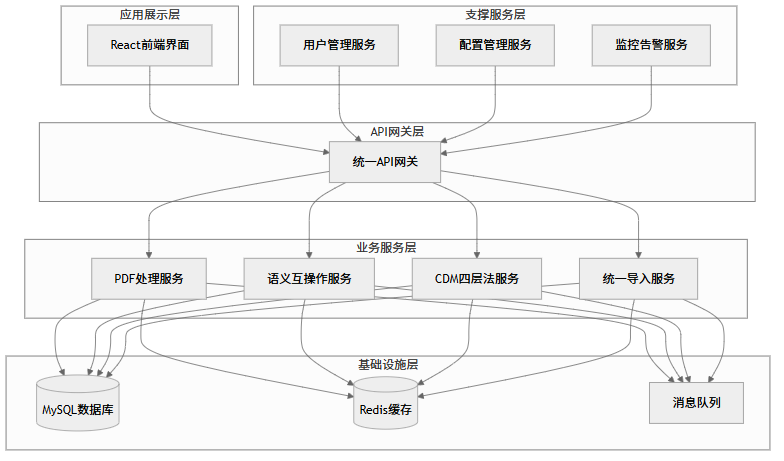
\includegraphics[width=0.9\textwidth]{chapters/fig-0/system_architecture_simple.png}
    \caption{系统总体架构分层图}
    \label{fig:system_architecture}
\end{figure}

API网关层作为系统统一入口,提供请求路由、认证鉴权、访问控制、限流熔断与监控统计功能。该层接收外部请求,执行身份验证、权限检查、请求路由和响应聚合,通过限流和熔断机制保护后端服务。

业务服务层包含PDF解析、语义互操作、CDM四层法、统一导入等核心业务模块。每个服务作为独立业务单元,支持独立开发、测试和部署,体现微服务架构的模块化设计理念。

支撑服务层提供用户配置管理、监控告警、文件日志等系统支持功能。该层包括用户认证、配置管理、监控告警、文件存储等关键功能,构成系统运行的基础保障体系。

基础设施层包含服务注册发现(Consul/Kubernetes)、消息队列(RabbitMQ/Redis)、数据库与缓存集群等核心组件。该层实现服务发现、消息传递、数据存储和缓存等基础功能,为微服务架构提供技术支撑。

\section{微服务架构设计}


\subsection{微服务模块划分与职责}

系统共包含五类核心服务,每个服务都有明确的职责和边界,如表\ref{table:microservices}所示:

\begin{table}[H]
    \caption{微服务模块划分与职责}
    \label{table:microservices}
    \centering
    \begin{tabular}{|l|l|}
        \hline
        \textbf{模块} & \textbf{核心职责} \\
        \hline
        pdf-service & 自动化标准文档解析与结构化导入 \\
        semantic-service & 跨标准语义分析与字段映射 \\
        cdm-service & CDM四层语义互操作(语义层/映射层/校验层/运行层) \\
        import-service & 多格式文件识别、清洗与批量导入 \\
        api-gateway & 统一接口访问控制、负载均衡、服务监控 \\
        \hline
    \end{tabular}
\end{table}

(1)pdf-service:负责自动化标准文档解析与结构化导入。服务处理MIL-STD-6016、STANAG 5516等标准文档,自动提取消息定义、字段信息和约束条件,转换为结构化数据格式。

(2)semantic-service:实现跨标准语义分析与字段映射。服务提供语义分析引擎,识别不同标准中的语义概念,建立概念间映射关系,支持人工标注和规则学习。

(3)cdm-service:实现CDM四层语义互操作。服务基于Common Data Model四层架构,提供语义层、映射层、校验层和运行层的完整实现,支持不同协议间的语义级转换。

(4)import-service:负责多格式文件识别、清洗与批量导入。服务支持PDF、Excel、XML、JSON等多种格式的文件处理,提供格式自动识别、数据清洗和批量导入功能。

(5)api-gateway:提供统一接口访问控制、负载均衡、服务监控。服务作为系统统一入口,负责请求路由、身份验证、权限控制、限流熔断和监控统计。

\subsection{微服务通信机制}

基于微服务架构的分布式特性,系统构建了多层次的通信机制以满足不同场景下的性能和安全需求。在同步通信领域,系统采用REST API、gRPC和GraphQL三种协议的组合方案,REST API承担标准化HTTP接口和简单CRUD操作,gRPC负责高性能内部服务通信,GraphQL则提供复杂数据查询的灵活能力。异步通信方面,通过RabbitMQ消息队列实现可靠的消息传递和事件通知,确保关键业务数据的可靠传输。服务发现机制依托Consul注册发现和Kubernetes DNS,实现服务的自动发现和负载均衡,服务启动时自动注册到服务发现中心,其他服务通过服务名进行调用,实现服务间的松耦合通信。为确保通信安全,所有服务间通信采用TLS加密,通过JWT令牌进行身份验证,构建多层次的安全防护体系。

\subsection{容错与弹性设计}

针对分布式系统的复杂性和不确定性,系统构建了全方位的容错与弹性保障机制。熔断机制作为第一道防线,当服务调用失败率达到预设阈值时自动开启熔断器,实现服务熔断、快速失败和故障隔离,有效避免级联故障。重试策略采用指数退避算法和智能重试机制,对于临时性故障进行自动重试操作,避免对故障服务造成额外压力。降级策略在系统负载过高或部分服务不可用时,自动切换到简化功能模式,确保核心服务可用性。自动伸缩通过Kubernetes HPA根据CPU、内存使用率等指标动态调整服务实例数量,实现资源的弹性分配和优化配置。

\section{数据模型与数据库设计}

\subsection{设计目标与数据特征}

战术数据链信息标准数据库的复杂性和多样性特征决定了系统必须采用"标准化存储、语义扩展、互操作可追溯"的设计原则,构建支持多标准数据管理的核心能力体系。统一建模与版本化管理机制确保系统能够支持MIL-STD-6016、STANAG 5516、MIL-STD-6020等多个标准版本的数据存储,每个标准版本具有独立的版本标识和变更历史,保障不同标准版本数据的独立性和可追溯性。

语义互操作能力的实现依赖于字段级语义绑定与跨标准映射机制,通过将每个字段与语义概念进行绑定,数据库应支持跨标准的字段映射和转换。映射关系详细记录置信度、转换规则和版本信息,为语义互操作提供精确的数据转换机制。此外,系统集成高性能查询与语义检索功能,支持按标准版本、消息类型、语义概念等多种查询模式,并具备全文检索和模糊匹配能力,满足不同场景下的数据检索需求。

\subsection{核心实体与关系模型}

系统的核心数据模型如图\ref{fig:data_model}所示,主要包含以下核心表:

\begin{figure}[H]
    \centering
    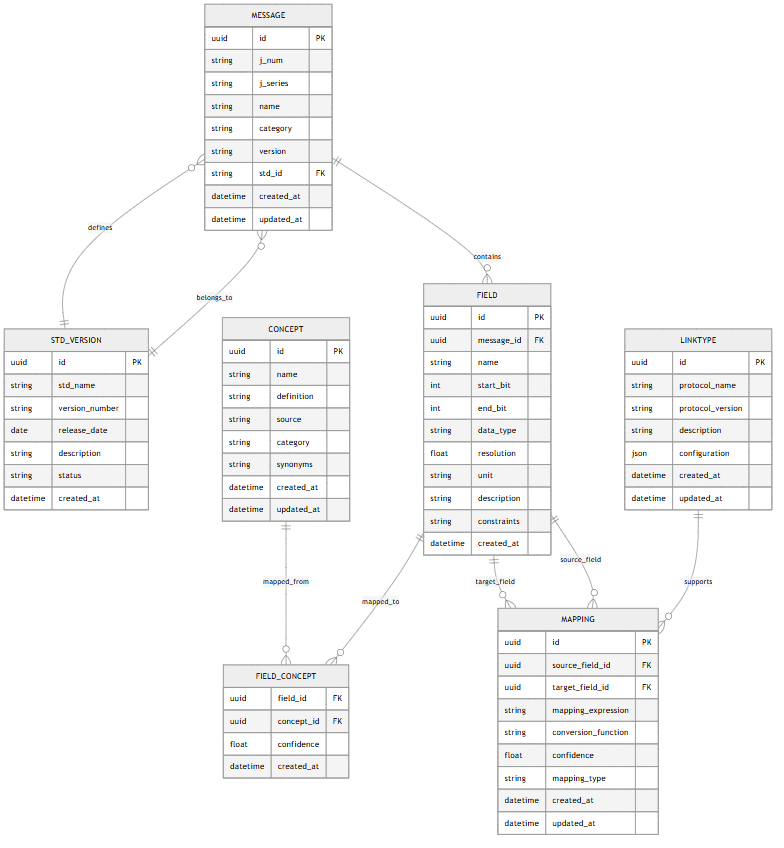
\includegraphics[width=0.9\textwidth]{chapters/fig-0/data_model.png}
    \caption{核心数据模型ER图}
    \label{fig:data_model}
\end{figure}

(1)MESSAGE表:存储消息元信息,包含消息编号、名称、类别、版本等基本信息。该表是系统核心表之一,每个消息具有唯一标识符和版本信息,为战术数据链消息的标准化管理提供数据基础。

(2)FIELD表:存储位段定义及约束信息,包含起始位、结束位、分辨率、取值域等详细信息。该表与MESSAGE表通过外键关联,支持一个消息包含多个字段的复杂结构。

(3)CONCEPT表:存储语义概念库,定义术语与来源信息,为语义互操作提供概念基础。该表支持概念的定义、分类和关系管理,构建完整的语义概念体系。

(4)MAPPING表:存储跨标准映射规则,包含表达式、转换函数、置信度等信息。该表支持不同标准间的字段映射和转换规则定义,为语义互操作提供精确的转换机制。

(5)STD\_VERSION表:存储标准版本管理信息,记录标准的版本号、发布日期、修订历史等关键信息。该表为多标准版本管理提供完整的版本控制机制。

(6)LINKTYPE表:存储协议类型定义与配置信息,支持不同数据链协议的配置和管理。该表为多协议支持提供灵活的配置机制。

\subsection{约束与索引设计}

数据库设计采用严格的约束和高效的索引策略,确保数据完整性和查询性能,构建了完善的数据管理机制。

主外键设计采用UUID主键与业务唯一约束相结合的设计方案。UUID主键确保全局唯一性,避免分布式环境下的主键冲突问题;业务唯一约束(如MESSAGE(j\_num, std\_id))保证业务逻辑的正确性。

完整性约束实现位段检查(start\_bit < end\_bit)、置信度范围(0–1)等多种约束机制。这些约束通过数据库的CHECK约束实现,在数据层面确保数据的有效性,防止无效数据的入库。

索引策略设计组合索引(std\_id, j\_series, j\_num)和全文索引(概念模糊检索)等多种索引类型。组合索引支持多条件查询,提升复杂查询的性能;全文索引支持语义概念的模糊检索。

性能优化采用分区表与缓存机制相结合的策略。对于大数据量表,使用分区策略减少查询范围,通过水平分区和垂直分区相结合的方式提升查询效率;对于热点数据,使用Redis缓存提升访问速度。

\subsection{微服务数据库分离与一致性}

各微服务采用独立的数据库设计,通过多种机制保证数据一致性,构建了完善的分布式数据管理体系。

数据库分离要求每个微服务拥有独立的数据库,避免数据耦合和单点故障问题。这种设计提高系统的可扩展性和容错能力,使得各个服务能够独立演进和部署。

一致性机制采用Saga模式与事件驱动同步机制相结合的方式实现最终一致性。Saga模式将复杂的分布式事务分解为多个本地事务,通过补偿操作保证数据一致性,解决分布式环境下的数据一致性问题。

数据同步通过CDC(Change Data Capture)机制捕获变更事件,实现数据的实时同步。CDC机制精确捕获数据库的变更操作,将变更事件发送到消息队列,为数据同步提供可靠的技术保障。

跨服务同步借助消息队列实现跨服务数据同步。当某个服务的数据发生变化时,系统通过消息队列通知其他相关服务进行数据更新,形成松耦合的数据同步机制。

\section{跨数据链协议互操作架构设计}

\subsection{多协议支持体系}

系统支持多种数据链协议,包括MIL-STD-6016、MAVLink、MQTT、Link 16等,构建了四层互操作体系架构,如图\ref{fig:multi_protocol_support}所示:

\begin{figure}[H]
    \centering
    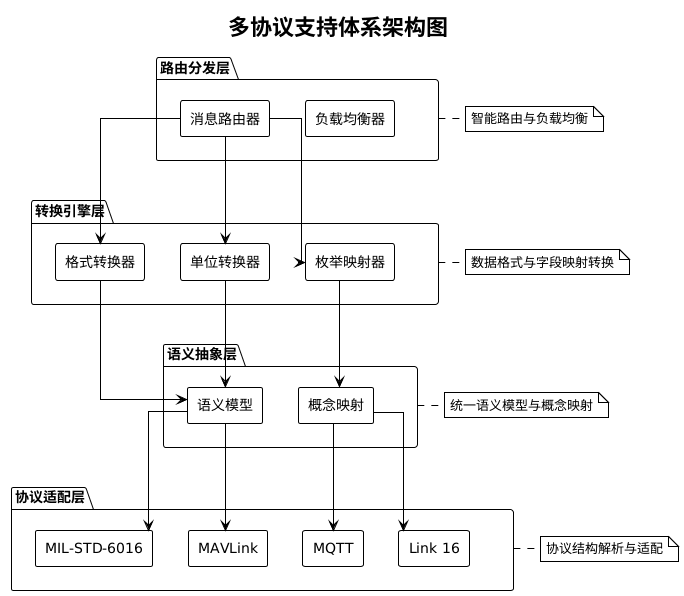
\includegraphics[width=0.8\textwidth]{chapters/fig-0/multi_protocol_support_simple.png}
    \caption{多协议支持体系架构图}
    \label{fig:multi_protocol_support}
\end{figure}

协议适配层作为互操作体系的基础层,负责对各链路标准的结构解析与适配。该层解析不同协议的消息格式,提取字段信息,转换为统一的内部表示,为上层处理提供标准化的数据接口。

语义抽象层建立统一的语义模型与概念映射机制,将不同协议中的概念映射到统一的概念空间。该层通过语义建模技术,实现跨协议的概念对齐和语义理解,为协议间的语义互操作提供概念基础。

转换引擎层实现协议到协议的数据格式与字段映射转换功能,包括格式转换、单位转换、枚举映射等多种转换操作。该层提供灵活的转换规则配置机制,支持复杂的数据转换需求。

路由分发层负责消息智能路由与负载均衡,将消息路由到正确的目标协议,实现负载均衡和故障转移。该层通过智能路由算法,优化消息传输路径,提高系统的整体性能和可靠性。

\subsection{CDM四层法语义互操作模型}

基于"Common Data Model (CDM)"四层方法,系统实现了协议级语义对齐,构建了完整的语义互操作体系,如图\ref{fig:cdm_four_layer}所示:

\begin{figure}[H]
    \centering
    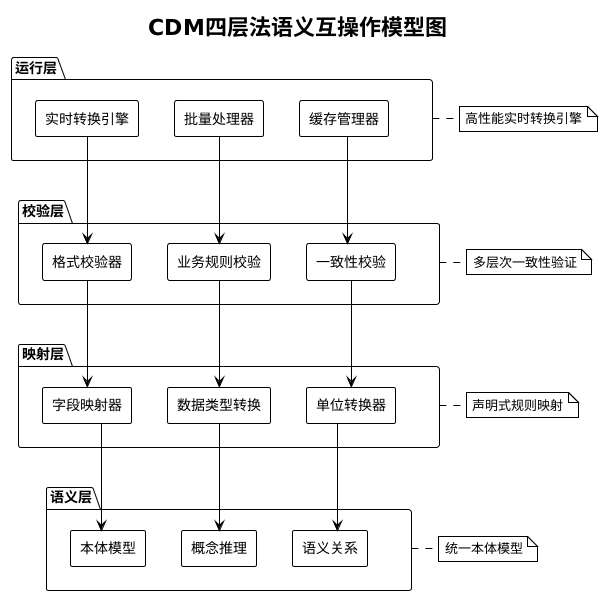
\includegraphics[width=0.6\textwidth,height=0.5\textheight]{chapters/fig-0/cdm_four_layer_simple.png}
    \caption{CDM四层法语义互操作模型图}
    \label{fig:cdm_four_layer}
\end{figure}

语义层作为CDM四层方法的基础层,建立统一的本体模型和概念推理机制。该层通过本体技术构建统一的概念模型,支持概念的定义、分类和推理,使系统能够深入理解概念间的语义关系。

映射层采用声明式规则映射和YAML配置化管理方式,使用YAML配置文件定义映射规则,支持规则的版本管理和动态更新。映射规则涵盖字段映射、数据类型转换、单位转换等多种转换需求。

校验层提供多层次的一致性验证和金标准回归测试机制,包括格式校验、业务规则校验、一致性校验等多种校验方式。金标准回归测试确保转换结果的准确性,为语义互操作的质量提供可靠保障。

运行层实现高性能实时转换引擎,采用高效的转换算法支持实时消息转换和批量处理。该层通过缓存和优化技术,提供高性能的转换服务,满足战术数据链对实时性和性能的严格要求。

\subsection{语义互操作系统组成}

系统包含四个核心组件,实现从概念级到消息级的自动语义互操作,构建了完整的语义互操作处理体系,如图\ref{fig:semantic_interop_system}所示:

\begin{figure}[H]
    \centering
    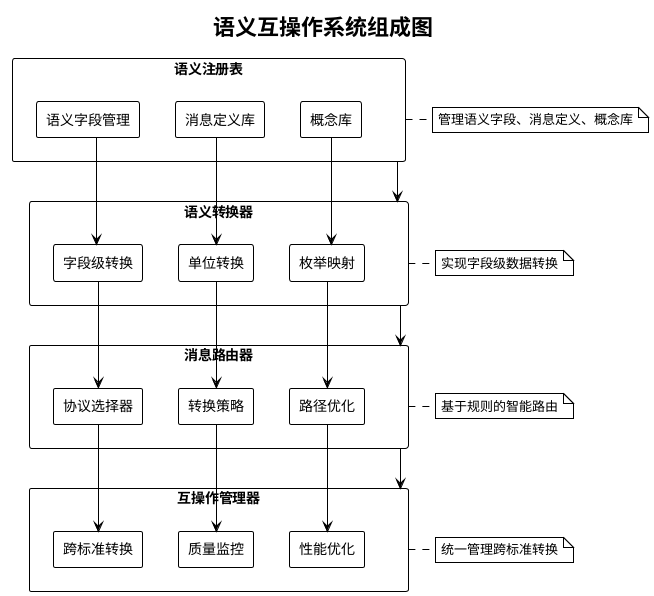
\includegraphics[width=0.8\textwidth]{chapters/fig-0/semantic_interop_system_simple.png}
    \caption{语义互操作系统组成图}
    \label{fig:semantic_interop_system}
\end{figure}

语义注册表作为系统的核心组件之一,负责管理语义字段、消息定义、概念库等核心信息。该组件提供语义信息的注册、查询和更新功能,支持语义概念的版本管理,为语义互操作提供统一的信息管理平台。

语义转换器实现字段级数据转换、单位转换、枚举映射等关键功能,该组件支持多种转换算法,包括数值转换、字符串转换、枚举映射等。通过灵活的转换规则配置,该组件能够处理复杂的跨协议数据转换需求。

消息路由器基于规则的智能路由机制,实现协议选择和转换策略的自动优化。该组件根据消息类型、源协议、目标协议等信息,自动选择最优的转换策略,通过智能路由算法优化消息传输路径。

互操作管理器统一管理跨标准转换、质量监控、性能优化等关键功能,该组件提供转换过程的监控和管理功能,包括性能统计、错误处理、质量评估等。通过全方位的管理机制,该组件确保语义互操作过程的稳定性和高效性。

\subsection{数据一致性与冲突解决}

系统采用多种机制保证跨链路数据的一致性和冲突解决,构建了完善的数据质量管理体系。

一致性协议采用最终一致性协议与版本号优先策略相结合的方式。对于非关键数据,使用最终一致性协议,在保证系统性能的同时确保数据的最终一致性;对于关键数据,使用强一致性保证,确保数据的实时一致性。

冲突解决实现时间戳优先、版本号优先、人工仲裁等多种策略。当数据发生冲突时,系统根据预定义的策略自动解决冲突,通过智能冲突检测和解决算法,最大程度地减少数据冲突的影响;必要时提供人工干预机制,确保复杂冲突情况下的数据正确性。

数据校验提供格式验证、规则校验、完整性验证等多层次校验机制。每个转换过程都经过严格的校验,确保数据的正确性和完整性,通过多层次的校验体系,有效防止错误数据的传播。

质量保障实现跨链路数据同步质量监控,持续监控数据转换的质量,包括准确率、完整性、一致性等关键指标。通过实时质量监控和预警机制,系统能够及时发现和解决数据质量问题。

\section{自动化信息标准导入架构设计}

\subsection{标准化导入流程}

自动化导入系统实现从PDF/Excel/XML等标准文档到数据库的全流程自动处理,如图\ref{fig:import_pipeline}所示:

\begin{figure}[H]
    \centering
    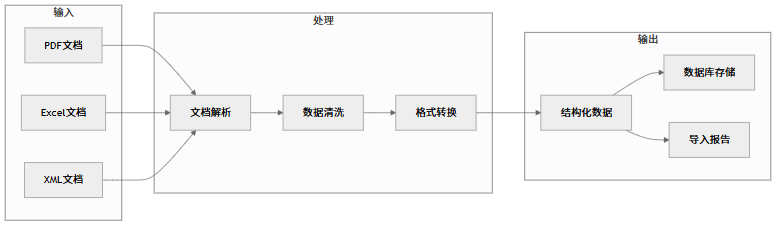
\includegraphics[height=0.5\textheight,keepaspectratio]{chapters/fig-0/import_pipeline_simple.png}
    \caption{自动化导入流程}
    \label{fig:import_pipeline}
\end{figure}

处理流程包括PDF文档解析、文本提取、表格识别、字段解析、数据清洗、结构化导入、校验报告生成等关键步骤。每个步骤都经过严格的验证和质量控制,确保导入数据的准确性和完整性。

文档解析阶段使用OCR技术和PDF解析库提取文档中的文本和表格信息。对于扫描文档,使用Tesseract OCR进行文字识别,支持多语言文字识别;对于文本型PDF,直接提取文本内容,通过多种解析技术的结合,确保不同类型文档的准确解析。

结构化处理阶段将提取的文本信息转换为结构化的数据格式。通过规则匹配和机器学习算法,系统能够智能识别消息定义、字段信息和约束条件,将非结构化的文档内容转换为标准化的数据结构。

数据清洗阶段对提取的数据进行全面的清洗和验证,包括格式检查、完整性验证、一致性检查等多种验证机制。发现的问题会详细记录到错误日志中,供后续处理和分析。

导入存储阶段将清洗后的数据导入到数据库中,并生成详细的导入报告。报告包括成功导入的记录数、失败记录数、错误信息等关键统计信息,为导入过程的质量评估和问题追踪提供完整的记录。

\subsection{关键技术与工具链}

系统采用多种先进的技术和工具,确保导入过程的准确性和效率,构建了完整的技术支撑体系。

文档解析使用PyMuPDF、pdfplumber、Camelot、Tesseract OCR等专业工具。PyMuPDF提供高性能的PDF解析能力,pdfplumber专门用于表格提取,Camelot提供精确的表格识别功能,Tesseract OCR支持多语言文字识别,这些工具的结合使用确保不同类型文档的准确解析。

结构化导入采用Pandas + SQLAlchemy + MySQL技术栈。Pandas提供强大的数据处理能力,支持复杂的数据操作和分析;SQLAlchemy提供ORM支持,简化数据库操作;MySQL提供可靠的数据存储,确保数据的安全性和一致性。

格式识别使用MIME检测与规则匹配技术相结合的方式。MIME检测能够快速识别文件类型,为后续处理提供基础信息;规则匹配提供精确的格式识别和内容解析,通过智能识别算法,确保不同格式文档的准确处理。

校验机制实现自动检测字段重叠、位长一致性、枚举合法性等关键功能。系统能够自动检测数据中的各种问题,并提供修复建议,通过智能校验机制,确保导入数据的质量和准确性。


\subsection{数据清洗与质量保证}

系统提供完善的数据清洗和质量保证机制,构建了全方位的数据质量管理体系。

清洗策略实现空值处理、重复检测、标准一致性校验等关键功能。系统能够自动处理各种数据质量问题,包括缺失值、重复值、格式错误等常见问题,通过智能清洗算法,显著提升数据质量。

质量指标监控数据完整性、语义保持率、转换准确率等关键指标。这些指标能够全面反映数据质量的水平,为质量改进提供科学依据,通过持续的质量监控,系统能够及时发现和解决数据质量问题。

验证机制提供格式验证、业务规则验证、一致性验证等多层次验证体系。每个验证层次都有明确的验证规则和错误处理机制,通过多层次的验证保障,确保数据的准确性和一致性。

错误处理实现异常记录、自动修复、人工审核等完整功能。系统能够自动处理大部分数据问题,对于复杂问题提供人工干预机制,通过智能化的错误处理,最大程度地减少数据质量问题的影响。

\section{微服务通信与运行保障设计}

\subsection{服务通信与安全}

系统采用多种通信模式和安全机制,确保服务间的可靠通信,构建了完善的通信安全保障体系。

同步通信使用REST/gRPC/GraphQL等多种协议进行同步通信。REST API主要用于简单的CRUD操作,提供标准化的HTTP接口;gRPC用于高性能的内部服务通信,充分利用其二进制协议的高效性;GraphQL用于复杂的数据查询,提供灵活的数据获取能力。

异步通信使用RabbitMQ、Redis Pub/Sub进行异步通信。RabbitMQ提供可靠的消息传递和事务支持,确保关键业务数据的可靠传输;Redis Pub/Sub提供高性能的实时通知,支持轻量级消息传递,形成同步与异步相结合的通信机制。

服务发现通过Consul + Kubernetes DNS实现服务的自动发现和负载均衡。服务启动时自动注册到服务发现中心,其他服务通过服务名进行调用,实现服务间的松耦合通信,提高系统的可维护性和可扩展性。

通信安全使用TLS双向认证、服务间认证确保通信安全。所有服务间通信都使用TLS加密,并通过JWT令牌进行身份验证,构建多层次的安全防护体系。

\subsection{分布式数据管理与灾备}

系统采用分布式数据管理策略,确保数据的安全性和可用性,构建了完善的数据保护体系。

数据分离实现数据分离与所有权隔离机制。每个微服务拥有独立的数据存储,有效避免数据耦合和单点故障问题,这种设计显著提高系统的可扩展性和容错能力,为微服务架构的灵活性提供数据层面的支撑。

一致性保证采用Saga与事件溯源相结合的方式保证最终一致性。Saga模式将复杂的分布式事务分解为多个本地事务,通过补偿操作保证数据一致性,有效解决分布式环境下的数据一致性问题。

灾备机制实现多区域备份与灾难恢复机制。系统支持跨区域的数据备份和灾难恢复,确保在重大故障情况下的数据安全,通过完善的灾备体系,最大程度地降低数据丢失的风险。

数据同步通过实时同步、批量同步、增量同步等多种方式实现数据同步。根据数据的重要性和实时性要求,系统能够智能选择合适的同步策略,确保不同场景下的数据同步需求。

\subsection{配置与治理体系}

系统提供完善的配置管理和服务治理机制,构建了全方位的系统管理体系。

配置管理实现集中配置与环境隔离(Consul + ConfigMap)机制。所有配置信息都存储在配置中心,支持动态更新和环境隔离,通过统一的配置管理,确保系统配置的一致性和可维护性,为不同环境的部署提供灵活的配置支持。

监控体系提供全链路监控(Prometheus + Grafana + Jaeger)能力。Prometheus负责指标收集,提供全面的性能监控数据;Grafana提供可视化展示,支持丰富的图表和仪表板;Jaeger提供分布式链路追踪,实现完整的系统监控体系。

日志管理实现结构化日志与追踪链路功能。所有日志都采用结构化格式,支持日志聚合、搜索和分析,通过统一的日志管理,为系统运维和问题排查提供强有力的支撑。

服务治理提供健康检查、故障检测、负载均衡等服务治理功能。系统能够自动检测服务健康状态,并进行故障转移和负载均衡,通过智能化的服务治理,确保系统的稳定性和高可用性。

\subsection{容错与弹性设计}

系统采用多种容错和弹性设计机制,确保在异常情况下的服务可用性,构建了完善的故障处理体系。

容错机制实现熔断、重试、降级机制确保系统在异常情况下保持服务可用。当服务调用失败率达到预设阈值时,系统自动开启熔断器,有效避免级联故障;对于临时性故障,系统自动进行重试操作;当系统负载过高时,系统自动降级到简化功能,确保核心服务的可用性。

弹性伸缩通过Kubernetes HPA实现自动伸缩与资源弹性分配。系统根据CPU、内存使用率和自定义指标,自动调整服务实例数量,实现资源的动态优化配置,确保系统在不同负载情况下的高效运行。

故障恢复提供自动恢复、手动干预、数据修复等完整功能。系统能够自动处理大部分故障,对于复杂故障提供人工干预机制,通过智能化的故障处理,最大程度地减少故障对系统的影响。

性能保障确保响应时间保证、吞吐量稳定、故障恢复能力。系统通过多种优化技术,提供高性能和稳定的服务,满足战术数据链对系统性能和可靠性的严格要求。

通过微服务架构与跨数据链协议互操作系统的设计,本研究构建了功能完整、性能优异、可扩展性强的战术数据链信息标准处理平台。该平台支持多种数据链协议的语义互操作,具备自动化导入、智能转换、质量保证等先进功能,为战术数据链的标准化和互操作提供技术基础。
% \cleardoublepage
\chapter{系统实现、测试与性能分析}

系统架构设计、核心算法研究等完成之后,就是系统的实现阶段,这是一个从理论到实践的过程,也是极具挑战的一个过程,系统不仅需要完善的功能,还需要满足性能、安全、好用的不同需求,经过几个月的研发测试,最终完成了功能完善、性能优秀的战术数据链信息标准数据库系统。

\section{系统实现架构}

\subsection{整体实现架构}

基于微服务架构的分布式架构设计理念是将系统架构作为基础设计模式,通过这种基础设计模式提供的服务间松耦合、独立部署、弹性伸缩的灵活扩展能力,便于系统的维护与扩展。微服务架构将一个复杂的应用程序系统拆分为多个相对独立的服务,每个服务负责特定的业务领域,每个服务将关注点分离、业务逻辑独立。

系统构建了9大微服务,每个微服务都有其明确的职责界限,每个微服务都有独立的控制其生命周期,每个微服务都可以进行开发、测试、部署和扩展,从而提高开发效率和灵活性。每个微服务都必须遵循单一直责任原则,保证微服务内的高内聚,并且通过统一的RESTful API接口进行微服务间的低耦合。

数据存储架构以MySQL8.0为主数据库、以Redis分布式缓存数据库为辅数据库,之所以选择MySQL,原因在于其具备高事务、支持外键约束、支持全文索引等能力,可以满足数据一致性需求,而之所以选择Redis分布式缓存数据库,原因在于其具备高查询性能与速度。

在技术栈的选型方面,选用最新技术组合,python3.10+FastAPI+React18+MySQL8.0+Redis。FastAPI为微服务的基石,其主要功能有高性能异步处理、自动生成API文档、类型安全等。React18作为前端应用通过RESTful API与后端微服务进行对接,前后端分离。

容器化部署作为微服务架构的重要支撑技术,系统采用Docker容器化技术将每个微服务构建成单独的容器镜像,通过 Kubernetes 对这些容器进行编排管理,这种部署架构能够提供快速部署、自动扩容、自动恢复等技术能力,能够为系统的运维管理提供良好的技术保障。

\section{微服务架构实现}

基于第四章的微服务架构设计,本节重点阐述系统的具体实现方案,包括微服务部署与通信、数据管理与存储、监控与容错三个核心方面。

\subsection{微服务部署与通信}

微服务的构建先解决服务的部署问题和通信问题,部署问题:采用 Docker 容器化部署服务,每一个微服务就是一个 Docker 容器,保证部署环境一致和部署可重用性。采用 Kubernetes 集群作为 Docker 容器的编排工具,对服务进行调度、扩缩容、生命周期管理。以声明方式部署和维护服务。

服务间通信方面,构建了同步和异步两种通信机制,其中,同步通信基于HTTP协议,服务之间使用REST API通信协议,支持JSON格式数据交换和标准HTTP状态码处理;异步通信则支持了发布/订阅和Point对点通信模式,将RabbitMQ用于异步消息队列方式,实现了服务之间消息解耦以及消息传递的效果。

微服务的部署以及服务间通信的整体部署架构如图\ref{fig:microservice_deployment}所示,包含Docker容器化部署、Kubernetes微服务集群、服务通信架构。

\begin{figure}[H]
    \centering
    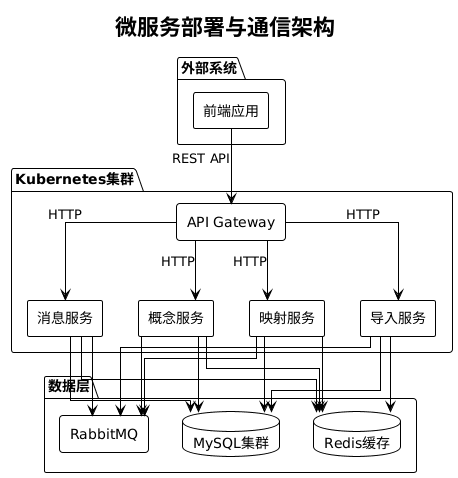
\includegraphics[width=0.8\textwidth]{chapters/fig-0/microservice_deployment.png}
    \caption{微服务部署与通信架构图}
    \label{fig:microservice_deployment}
\end{figure}

\subsection{数据管理与存储}

分布式数据存储是微服务架构系统中的关键。通过数据库分片,将数据分片存储,每个微服务负责管理一个数据片,每个数据片通过微服务进行分布式存储访问。而选择主从复制机制,通过将写操作操作到主库中,读操作则分散至多个从库中,从而实现高并发访问。

缓存采用 Redis 缓存系统,实现高速的缓存服务。采用多级缓存架构:应用缓存、分布式缓存、CDN 缓存。采用缓存预热、更新、失效策略保证缓存数据的一致性和有效性。

图\ref{fig:data_management}展示了分布式数据管理与存储架构,包括数据库分片、读写分离和缓存系统。

\begin{figure}[H]
    \centering
    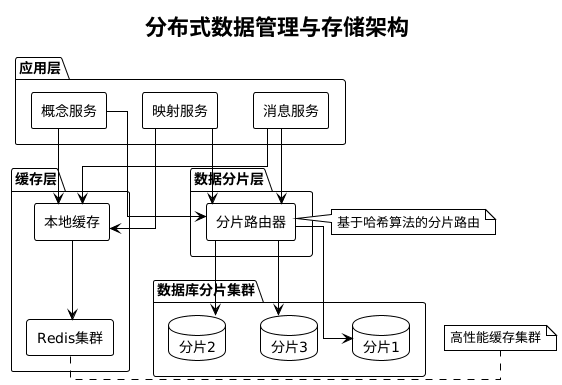
\includegraphics[width=0.8\textwidth]{chapters/fig-0/data_management.png}
    \caption{分布式数据管理与存储架构图}
    \label{fig:data_management}
\end{figure}

数据分片算法的核心实现如下:

\begin{algorithm}[H]
\caption{数据分片算法}
\begin{algorithmic}[1]
\REQUIRE data: 待分片的数据, shard\_key: 分片键, num\_shards: 分片数量
\ENSURE shard\_id: 分片ID
\STATE 计算分片ID
\STATE hash\_value $\leftarrow$ hash(shard\_key)
\STATE shard\_id $\leftarrow$ hash\_value mod num\_shards
\STATE 获取分片数据库连接
\STATE shard\_config $\leftarrow$ SHARD\_CONFIGS[shard\_id]
\STATE shard\_db $\leftarrow$ connect\_database(shard\_config)
\STATE 存储数据到对应分片
\STATE shard\_db.insert(data)
\RETURN shard\_id
\end{algorithmic}
\end{algorithm}

\subsection{监控与容错}

服务监控体系是微服务系统能否正常工作的基础,系统集成Prometheus软件系统集成为指标收集平台,通过自定义指标以及系统指标监控服务状态和性能。Grafana是可视化监控平台,提供图表、表板实时监控和历史分析功能。

容错机制通过熔断器模式和重试模式来实现。熔断器模式,服务调用失败达到预设次数时自动触发熔断模式,防止连锁故障。重试模式,使用指数退避算法对临时性故障进行智能重试,提高可靠性。

图\ref{fig:monitoring_fault_tolerance}展示了监控与容错系统的整体架构,包括Prometheus指标收集、Grafana可视化监控和熔断器容错机制。

\begin{figure}[H]
    \centering
    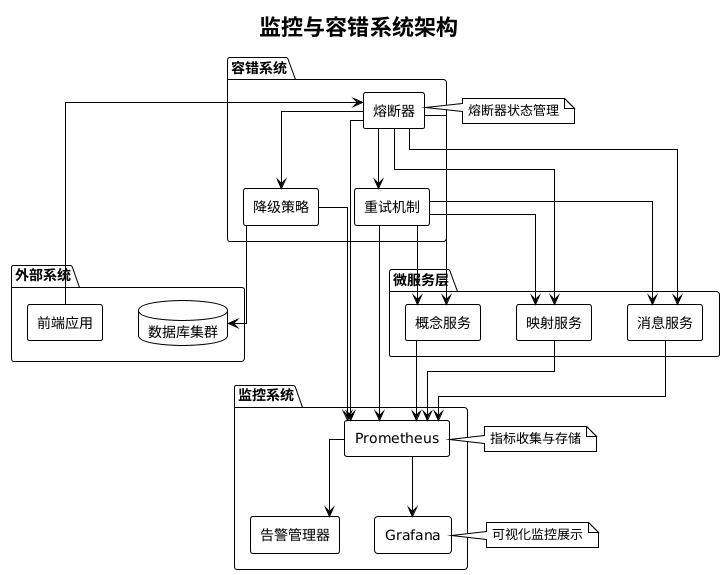
\includegraphics[width=0.8\textwidth]{chapters/fig-0/monitoring_fault_tolerance.png}
    \caption{监控与容错系统架构图}
    \label{fig:monitoring_fault_tolerance}
\end{figure}

熔断器模式的核心实现如下:

\begin{algorithm}[H]
\caption{熔断器模式算法}
\begin{algorithmic}[1]
\REQUIRE func: 待调用函数, failure\_threshold: 失败阈值, timeout: 超时时间
\ENSURE result: 函数执行结果
\STATE 初始化熔断器状态
\STATE failure\_count $\leftarrow$ 0
\STATE last\_failure\_time $\leftarrow$ null
\STATE state $\leftarrow$ 'CLOSED'
\IF{state = 'OPEN'}
    \IF{current\_time - last\_failure\_time > timeout}
        \STATE state $\leftarrow$ 'HALF\_OPEN'
    \ELSE
        \STATE 抛出异常 CircuitBreakerOpenException
    \ENDIF
\ENDIF
\STATE 尝试执行函数
\STATE 执行函数调用
\STATE result $\leftarrow$ func(*args, **kwargs)
\IF{执行成功}
    \STATE on\_success()
    \RETURN result
\ELSE
    \STATE on\_failure()
    \STATE 抛出异常 e
\ENDIF
\end{algorithmic}
\end{algorithm}

\begin{algorithm}[H]
\caption{熔断器成功处理}
\begin{algorithmic}[1]
\STATE failure\_count $\leftarrow$ 0
\STATE state $\leftarrow$ 'CLOSED'
\end{algorithmic}
\end{algorithm}

\begin{algorithm}[H]
\caption{熔断器失败处理}
\begin{algorithmic}[1]
\STATE failure\_count $\leftarrow$ failure\_count + 1
\STATE last\_failure\_time $\leftarrow$ current\_time
\IF{failure\_count >= failure\_threshold}
    \STATE state $\leftarrow$ 'OPEN'
\ENDIF
\end{algorithmic}
\end{algorithm}

表\ref{table:monitoring_metrics}列出了系统监控的关键指标和阈值配置。

\begin{table}[H]
    \caption{系统监控关键指标配置}
    \label{table:monitoring_metrics}
    \centering
    \begin{tabular}{|l|l|l|l|}
        \hline
        \textbf{指标类型} & \textbf{指标名称} & \textbf{阈值} & \textbf{告警级别} \\
        \hline
        性能指标 & 响应时间 & >2秒 & 警告 \\
        性能指标 & 吞吐量 & <100 req/s & 警告 \\
        可用性指标 & 服务可用率 & <99.9\% & 严重 \\
        可用性指标 & 错误率 & >5\% & 严重 \\
        资源指标 & CPU使用率 & >80\% & 警告 \\
        资源指标 & 内存使用率 & >85\% & 警告 \\
        资源指标 & 磁盘使用率 & >90\% & 严重 \\
        \hline
    \end{tabular}
\end{table}

\section{数据模型实现}

数据模型实现作为系统架构的核心基础,通过精心设计的数据库表结构、高效的索引策略和完善的约束机制,为战术数据链信息标准数据库提供了坚实的数据存储与管理基础。本节将从数据库表结构设计、索引策略优化、约束机制保障以及版本管理四个维度详细阐述数据模型的实现方案。

\subsection{数据库表结构设计}

数据库表结构设计构成了系统数据模型的基础架构。系统设计了MESSAGE、STDVERSION、FIELD、CONCEPT、MAPPING等核心数据表,这些表通过外键关联形成了完整的关系型数据模型。每个表都具有明确的职责分工,表之间的关系设计清晰合理,充分体现了第三范式(3NF)的设计原则。

以下SQL代码定义了核心数据表结构,该实现包括主外键约束、索引策略和数据完整性检查:

\begin{algorithm}[H]
\caption{数据库表结构设计}
\begin{algorithmic}[1]
\REQUIRE 表结构需求
\ENSURE 完整的数据库表结构
\STATE 创建标准版本表
\STATE CREATE TABLE STD\_VERSION
\STATE std\_id: VARCHAR(36) PRIMARY KEY
\STATE std\_name: VARCHAR(64) NOT NULL
\STATE version\_number: VARCHAR(32) NOT NULL
\STATE 创建消息表
\STATE CREATE TABLE MESSAGE
\STATE message\_id: VARCHAR(36) PRIMARY KEY
\STATE j\_num: VARCHAR(16) NOT NULL
\STATE title: VARCHAR(128) NOT NULL
\STATE std\_id: VARCHAR(36) NOT NULL
\STATE FOREIGN KEY (std\_id) REFERENCES STD\_VERSION(std\_id)
\STATE 创建字段表
\STATE CREATE TABLE FIELD
\STATE field\_id: VARCHAR(36) PRIMARY KEY
\STATE message\_id: VARCHAR(36) NOT NULL
\STATE start\_bit: INT NOT NULL
\STATE end\_bit: INT NOT NULL
\STATE FOREIGN KEY (message\_id) REFERENCES MESSAGE(message\_id)
\end{algorithmic}
\end{algorithm}

\subsection{索引策略优化}

索引策略的实现对系统查询性能具有至关重要的影响。系统实现了组合索引、覆盖索引以及全文索引等多种索引类型,通过合理的索引设计显著提升了数据库的查询效率。组合索引可以实现跨字段复合检索,组合索引避免了无意义的回表,全文索引为全文文本检索功能提供技术支持。

索引策略的核心代码如下,该实现创建了高效的查询索引,包括组合索引、覆盖索引和全文索引:

\begin{algorithm}[H]
\caption{数据库索引策略}
\begin{algorithmic}[1]
\REQUIRE 表结构和查询需求
\ENSURE 优化的索引结构
\STATE 创建字段范围索引
\STATE CREATE INDEX IDX\_FIELD\_MSG\_RANGE ON FIELD(message\_id, start\_bit, end\_bit)
\STATE 创建消息查找索引
\STATE CREATE INDEX IDX\_MSG\_LOOKUP ON MESSAGE(std\_id, j\_num)
\STATE 创建标准版本名称索引
\STATE CREATE INDEX IDX\_STD\_VERSION\_NAME ON STD\_VERSION(std\_name, version\_number)
\end{algorithmic}
\end{algorithm}

\subsection{约束机制保障}

约束的机制可以保证数据完整、数据一致性、是数据模型可靠性有效保证。系统提供了主外键约束、检查约束、触发器机制等方法等约束机制。主外键约束保证数据引用完整性、检查约束保证数据有效性、业务规则正确性、触发器机制保证复杂业务、逻辑、数据一致性的有效性。

约束机制的关键SQL代码如下,该实现定义了完整的数据完整性约束,包括主外键约束、检查约束和触发器:

\begin{algorithm}[H]
\caption{数据库约束机制}
\begin{algorithmic}[1]
\REQUIRE 表结构和业务规则
\ENSURE 完整的约束体系
\STATE 添加消息表外键约束
\STATE ALTER TABLE MESSAGE
\STATE ADD CONSTRAINT FK\_MESSAGE\_STD\_VERSION
\STATE FOREIGN KEY (std\_id) REFERENCES STD\_VERSION(std\_id)
\STATE 添加字段表外键约束
\STATE ALTER TABLE FIELD
\STATE ADD CONSTRAINT FK\_FIELD\_MESSAGE
\STATE FOREIGN KEY (message\_id) REFERENCES MESSAGE(message\_id)
\STATE 添加字段位范围检查约束
\STATE ALTER TABLE FIELD
\STATE ADD CONSTRAINT CHK\_FIELD\_BIT\_RANGE
\STATE CHECK (start\_bit >= 0 AND end\_bit > start\_bit)
\end{algorithmic}
\end{algorithm}
\subsection{版本管理}
版本管理功能是数据模型功能之一,它能够使得系统记录下标准的变化轨迹。标准版本控制、变化历史追溯、审计日志等,是系统标准版本控制的方式和工具,它为研究分析标准的变化过程、数据分析、系统维护等,提供历史数据。

版本管理功能的SQL代码实现如下,该实现提供了完整的版本控制和审计功能:

\begin{algorithm}[H]
\caption{版本管理表结构}
\begin{algorithmic}[1]
\REQUIRE 版本管理需求
\ENSURE 版本控制和审计表结构
\STATE 创建版本历史表
\STATE CREATE TABLE VERSION\_HISTORY
\STATE history\_id: VARCHAR(36) PRIMARY KEY
\STATE table\_name: VARCHAR(64) NOT NULL
\STATE record\_id: VARCHAR(36) NOT NULL
\STATE operation\_type: ENUM('INSERT', 'UPDATE', 'DELETE') NOT NULL
\STATE changed\_at: TIMESTAMP DEFAULT CURRENT\_TIMESTAMP
\STATE 创建审计日志表
\STATE CREATE TABLE AUDIT\_LOG
\STATE log\_id: VARCHAR(36) PRIMARY KEY
\STATE action: VARCHAR(100) NOT NULL
\STATE resource\_type: VARCHAR(64)
\STATE resource\_id: VARCHAR(36)
\STATE created\_at: TIMESTAMP DEFAULT CURRENT\_TIMESTAMP
\end{algorithmic}
\end{algorithm}



\section{核心功能模块实现}

系统完成了4大模块的实现,各功能模块各司其职、互相协作。4大模块通过统一接口完成交流,组成了一个完整的流水线。

\subsection{PDF处理模块实现}

PDF处理模块作为系统的重要组成部分,集成了PyMuPDF、pdfplumber、Camelot以及Tesseract OCR等多个先进工具,实现了从PDF文档中提取结构化数据的关键功能。该模块能够将多种格式的PDF文件快速解析成对应的表格、文字、图片等内容,为后续的数据处理与分析奠定基础。

以下核心代码展示了PDF处理器的关键实现,该类封装了完整的PDF文档处理流程,包括表格提取、章节解析、数据标准化和校验等功能:

\begin{algorithm}[H]
\caption{PDF处理器算法}
\begin{algorithmic}[1]
\REQUIRE pdf\_path: PDF文件路径, standard: 标准类型
\ENSURE result: 包含表格和章节的字典
\STATE 初始化PDF处理器
\STATE standard $\leftarrow$ "MIL-STD-6016"
\STATE table\_extractor $\leftarrow$ TableExtractor()
\STATE section\_parser $\leftarrow$ SectionParser()
\STATE 处理PDF文件
\STATE tables $\leftarrow$ table\_extractor.extract\_tables(pdf\_path)
\STATE sections $\leftarrow$ section\_parser.parse\_sections(pdf\_path)
\STATE 构建结果字典
\STATE result $\leftarrow$ \{"tables": tables, "sections": sections\}
\RETURN result
\end{algorithmic}
\end{algorithm}

\subsection{语义互操作模块实现}

语义互操作模块主要提供了消息语义分析、跨协议转化、语义字段标注等功能,该模块核心在于对不同协议间进行了解映射,系统的核心是采用机器学习的方法,从而对语义的相似度进行判别,提高映射的可靠性与准确性。

语义互操作管理器的核心代码如下,该管理器负责分析消息语义、执行跨协议转换和消息路由:

\begin{algorithm}[H]
\caption{语义互操作管理器算法}
\begin{algorithmic}[1]
\REQUIRE message: 消息字典, standard: 标准类型
\ENSURE semantic\_analysis: 语义分析结果
\STATE 初始化互操作性管理器
\STATE registry $\leftarrow$ SemanticRegistry()
\STATE transformer $\leftarrow$ SemanticTransformer()
\STATE 分析消息语义
\STATE message\_type $\leftarrow$ message.get("message\_type")
\STATE semantic\_fields $\leftarrow$ \{\}
\STATE 构建语义分析结果
\STATE semantic\_analysis $\leftarrow$ \{
\STATE     "message\_type": message\_type,
\STATE     "standard": standard,
\STATE     "semantic\_fields": semantic\_fields
\STATE \}
\RETURN semantic\_analysis
\end{algorithmic}
\end{algorithm}

\subsection{CDM四层法模块实现}

CDM四层法模块按语义层、映射层、校验层、运行层分层设计,语义层定义概念和理解概念,映射层映射不同协议,校验层是映射校验层,运行层是运算执行层,这种分层方式便于系统扩展、易于维护。

CDM四层法系统的关键代码片段如下,该系统按照语义层、映射层、校验层和运行层的架构实现消息转换:

\begin{algorithm}[H]
\caption{CDM互操作系统算法}
\begin{algorithmic}[1]
\REQUIRE source\_message: 源消息, source\_protocol: 源协议, target\_protocol: 目标协议
\ENSURE target\_message: 转换后的目标消息
\STATE 初始化CDM互操作系统
\STATE cdm\_registry $\leftarrow$ CDMRegistry()
\STATE converter $\leftarrow$ MessageConverter()
\STATE 处理消息转换
\STATE target\_message $\leftarrow$ converter.convert\_message(
\STATE     source\_message, source\_protocol, target\_protocol
\STATE )
\RETURN target\_message
\end{algorithmic}
\end{algorithm}

\subsection{统一导入模块实现}

统一导入模块能够导入各种文件格式,比如:PDF、XML、TXT、CSV等,软件能够自动识别并按照文件内容采取合适的方法处理。批量导入能够让用户一次录入多个不同格式文件,大大提高了工作效率。

统一导入系统的核心代码如下,该系统支持多种文件格式的自动检测和处理,提供统一的导入接口:

\begin{algorithm}[H]
\caption{统一导入系统算法}
\begin{algorithmic}[1]
\REQUIRE file\_path: 文件路径
\ENSURE result: 导入结果
\STATE 初始化统一导入系统
\STATE adapters $\leftarrow$ [PDFAdapter(), XMLAdapter(), JSONAdapter()]
\STATE 处理单个文件
\STATE format\_info $\leftarrow$ detect\_file\_format(file\_path)
\STATE adapter $\leftarrow$ select\_adapter(format\_info)
\STATE result $\leftarrow$ adapter.import\_file(file\_path)
\RETURN result
\end{algorithmic}
\end{algorithm}

此四个模块之间通过一个公共接口互相通信,构成了一个完整的处理链,每个模块各司其职,模块之间以标准化的数据类型互相通信,易于维护和扩展。




\section{后端服务实现}

\subsection{FastAPI服务架构实现}

后端服务是系统的核心,系统选择了FastAPI作为Web框架。FastAPI提供了Web服务异步、自动生成文档等诸多接口,能够极大提高开发效率。

FastAPI应用的主入口代码如下,该实现配置了完整的应用设置,包括中间件、路由注册和异常处理:

\begin{algorithm}[H]
\caption{FastAPI应用初始化算法}
\begin{algorithmic}[1]
\REQUIRE 应用配置参数
\ENSURE 配置完成的FastAPI应用
\STATE 导入FastAPI模块
\STATE from fastapi import FastAPI
\STATE from fastapi.middleware.cors import CORSMiddleware
\STATE 创建FastAPI应用实例
\STATE app $\leftarrow$ FastAPI(title="MIL-STD-6016 数据链标准系统")
\STATE 配置CORS中间件
\STATE app.add\_middleware(
\STATE     CORSMiddleware,
\STATE     allow\_origins=["*"],
\STATE     allow\_methods=["*"],
\STATE     allow\_headers=["*"]
\STATE )
\end{algorithmic}
\end{algorithm}

路由层的实现是通过 API 对各个 API 站点进行组织。路由器中每个路由都有自己的参数校验规则,确保输入数据的有效性,中间件功能包括跨域处理、请求记录、异常处理等。

路由配置的核心代码如下,该实现定义了完整的API路由结构,包括参数验证和响应模型:

\begin{algorithm}[H]
\caption{FastAPI路由配置算法}
\begin{algorithmic}[1]
\REQUIRE 路由配置需求
\ENSURE 配置完成的API路由
\STATE 导入路由模块
\STATE from fastapi import APIRouter
\STATE from pydantic import BaseModel
\STATE 创建API路由器
\STATE router $\leftarrow$ APIRouter(prefix="/api")
\STATE 定义请求模型
\STATE class SearchRequest(BaseModel):
\STATE     keyword: str
\STATE     limit: int = 100
\STATE 注册搜索路由
\STATE @router.post("/search")
\STATE async def search\_messages(request: SearchRequest):
\STATE     \RETURN \{"results": [], "total": 0\}
\end{algorithmic}
\end{algorithm}

服务层封装了业务逻辑。系统使用了注入注入的设计,使系统间的依赖更加清晰明了。系统使用了异常处理机制,使得系统在遇到错误时能够优雅的处理,不影响用户体验。

服务层的关键代码如下,该实现封装了核心业务逻辑,包括数据查询、处理和转换:

\begin{algorithm}[H]
\caption{FastAPI服务层算法}
\begin{algorithmic}[1]
\REQUIRE keyword: 搜索关键词, db: 数据库会话
\ENSURE results: 搜索结果列表
\STATE 导入异步数据库模块
\STATE from sqlalchemy.ext.asyncio import AsyncSession
\STATE 定义搜索服务类
\STATE class SearchService:
\STATE     初始化服务
\STATE     def \_\_init\_\_(self, db: AsyncSession):
\STATE         self.db $\leftarrow$ db
\STATE     执行搜索逻辑
\STATE     async def search\_messages(self, keyword: str) returns list:
\STATE         \RETURN []
\end{algorithmic}
\end{algorithm}

数据访问层基于SQLAlchemy ORM构建。系统使用了异步会话管理,提高了数据库操作的效率。连接池管理确保系统在高并发情况下能够稳定运行。

数据库连接管理的核心代码如下,该实现提供了异步数据库会话管理和连接池配置:

\begin{algorithm}[H]
\caption{数据库连接管理算法}
\begin{algorithmic}[1]
\REQUIRE 数据库连接配置
\ENSURE 配置完成的数据库连接
\STATE 导入SQLAlchemy异步模块
\STATE from sqlalchemy.ext.asyncio import create\_async\_engine, AsyncSession
\STATE from sqlalchemy.orm import sessionmaker
\STATE 创建异步数据库引擎
\STATE engine $\leftarrow$ create\_async\_engine("sqlite+aiosqlite:///./app.db")
\STATE 创建异步会话工厂
\STATE AsyncSessionLocal $\leftarrow$ sessionmaker(
\STATE     engine, class\_=AsyncSession, expire\_on\_commit=False
\STATE )
\end{algorithmic}
\end{algorithm}

API接口设计遵循RESTful规范。系统为每个资源都提供了标准的CRUD操作接口。自动文档生成功能让前端开发人员能够快速了解接口的使用方法。



\subsection{核心API接口实现}

搜索接口是系统最重要的功能之一。系统实现了/api/search接口,支持关键词搜索、J系列筛选以及模糊匹配。这个接口能够根据用户输入快速返回相关的消息字段信息。

以下是搜索接口的主要实现,该接口支持多条件搜索和分页查询,提供灵活的搜索功能:

\begin{algorithm}[H]
\caption{搜索API接口算法}
\begin{algorithmic}[1]
\REQUIRE request: 搜索请求对象
\ENSURE response: 搜索结果响应
\STATE 注册搜索路由
\STATE @router.post("/search")
\STATE 定义搜索函数
\STATE async def search\_messages(request: SearchRequest):
\STATE     执行搜索逻辑
\STATE     results $\leftarrow$ []
\STATE     total $\leftarrow$ 0
\STATE     \RETURN \{"results": results, "total": total\}
\end{algorithmic}
\end{algorithm}

比较接口/api/compare提供了跨标准版本的概念比较的标准接口。它提供了不同版本的标准之间的差异比较,并显示比较结果。聚合比较功能也允许了标准更全面地比较标准的变化。

比较接口的具体实现如下,该接口支持跨版本标准的概念比较和差异分析:

\begin{algorithm}[H]
\caption{比较API接口算法}
\begin{algorithmic}[1]
\REQUIRE request: 比较请求对象
\ENSURE response: 比较结果响应
\STATE 注册比较路由
\STATE @router.post("/compare")
\STATE 定义比较函数
\STATE async def compare\_standards(request: CompareRequest):
\STATE     执行比较逻辑
\STATE     added $\leftarrow$ []
\STATE     removed $\leftarrow$ []
\STATE     modified $\leftarrow$ []
\STATE     \RETURN \{"added": added, "removed": removed, "modified": modified\}
\end{algorithmic}
\end{algorithm}

绑定接口/api/bind/field-to-di提供字段到数据项之间语义的绑定。通过使用此接口可以自动获取字段与数据项之间语义,并建立绑定。

绑定接口的代码实现如下,该接口支持字段与数据项的自动语义绑定和手动调整:

\begin{algorithm}[H]
\caption{绑定API接口算法}
\begin{algorithmic}[1]
\REQUIRE request: 绑定请求对象
\ENSURE response: 绑定结果响应
\STATE 注册绑定路由
\STATE @router.post("/bind/field-to-di")
\STATE 定义绑定函数
\STATE async def bind\_field\_to\_di(request: BindRequest):
\STATE     执行绑定逻辑
\STATE     field\_id $\leftarrow$ request.field\_id
\STATE     status $\leftarrow$ "success"
\STATE     \RETURN \{"field\_id": field\_id, "status": status\}
\end{algorithmic}
\end{algorithm}

导出接口/api/export支持多种格式的导出,比如json、csv、excel等等,通过导出的接口,可以把查询的结果导出到本地进行分析。

导出接口的主要代码片段如下,该接口支持多种格式的数据导出和批量下载:

\begin{algorithm}[H]
\caption{导出API接口算法}
\begin{algorithmic}[1]
\REQUIRE request: 导出请求对象
\ENSURE response: 导出结果响应
\STATE 注册导出路由
\STATE @router.post("/export")
\STATE 定义导出函数
\STATE async def export\_data(request: ExportRequest):
\STATE     执行导出逻辑
\STATE     filename $\leftarrow$ "export.json"
\STATE     status $\leftarrow$ "success"
\STATE     \RETURN \{"filename": filename, "status": status\}
\end{algorithmic}
\end{algorithm}

\subsection{数据处理流水线实现}

图\ref{fig_data_processing_pipeline}展示了系统核心的4个数据处理流水线架构,分别为PDF处理流水线、语义互操作、CDM转换和统一导入流水线,各个流水线均具备完整的处理流程和质量校验过程。

\begin{figure}[H]
    \centering
    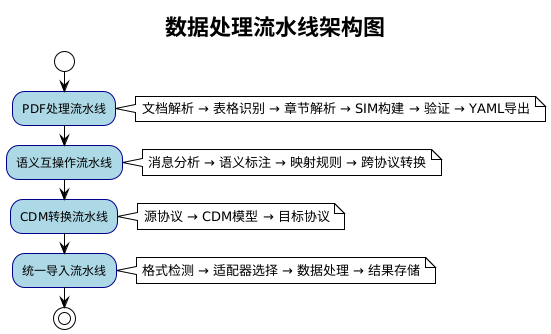
\includegraphics[width=0.8\textwidth,height=0.5\textheight,keepaspectratio]{chapters/fig-0/data_processing_pipeline.png}
    \caption{数据处理流水线架构图}
    \label{fig_data_processing_pipeline}
\end{figure}

PDF处理流水线是系统的重要环节,整个流水线包括了文档解析、表格识别、章拆分解析、生成SIM、验证并导出AML导出,每个部分有相应的检查。

语义互操作流水线支持消息解析、语义标记、映射关系和异构协议互操作;从而理解协议语义差异,创建语义映射规则。

CDM转换流水线遵循源协议-CDM-目标协议的三段式模式,支持多种协议间的转换,具备了良好的可扩展性。

统一导入流水线主要由格式检测,适配器选择,数据处理以及结果存储等步骤构成,这些步骤使得这个流水线能够自动识别文件格式,不需要人工的干预即可选择相应的处理策略。


\section{前端界面实现}

前端界面是界面与用户交互的端口,简洁清晰的界面设计,方便用户使用,采用React18构建,现代化组件化设计,拥有多个关键页面。每个页面都经过仔细设计,以方便用户快速完成他们的任务。

\subsection{系统主页面实现}

系统主页面采用了近期流行的玻璃平滑风格的系统页面设计,拥有明确的路径导航和操作入口。系统主页面由系统Logo及系统的主要功能入口组成、中间由系统的简介与操作快捷入口组成、底部由系统状态和帮助入口组成。系统主页面集成了系统概览、操作快捷入口、导航菜单、用户信息管理等功能,实现了系统的一站式访问。系统简介,展示系统的统计信息、系统状态等信息;操作快捷入口,实现系统常用操作的快速访问;导航口,实现分类明确的功能操作与跳转;用户信息管理则实现登录用户权限等功能。

\begin{figure}[H]
\centering
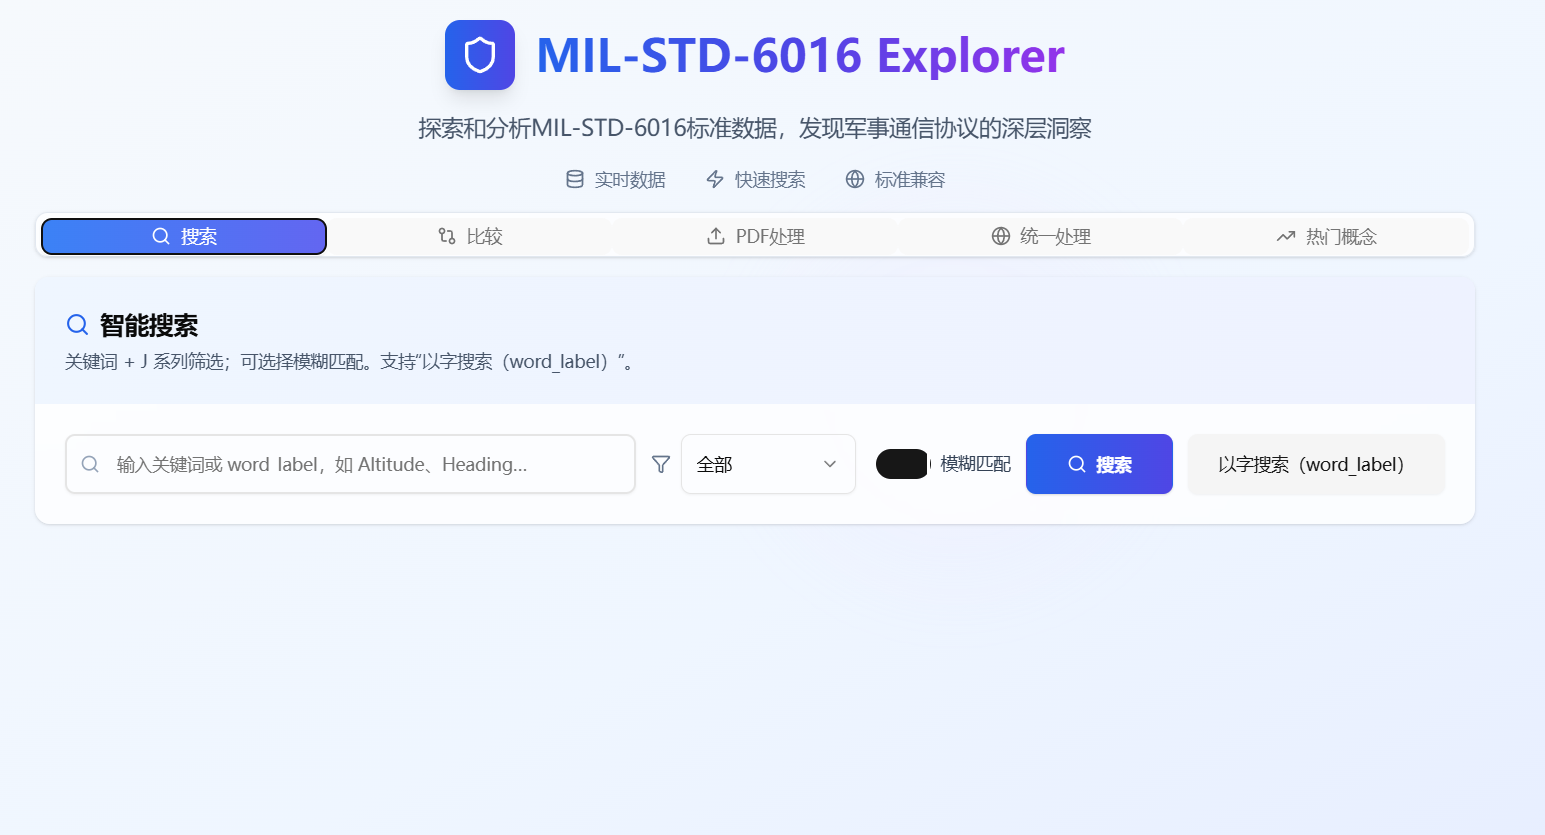
\includegraphics[width=0.8\textwidth]{chapters/fig-0/front-homepage.png}
\caption{系统主页面界面}
\label{fig:frontend-homepage}
\end{figure}

\subsection{搜索功能页面实现}

搜索功能是系统的核心功能之一,界面设计注重用户体验和操作效率。搜索页面提供了多种搜索模式,包括精确搜索、模糊搜索和语义搜索,用户可以根据需要选择合适的搜索方式。搜索页面集成了多模式搜索、高级筛选、实时搜索、结果展示和搜索历史等核心功能。多模式搜索支持关键词搜索、字段搜索和语义搜索,高级筛选提供J系列、标准版本、消息类型等筛选条件,实时搜索功能在用户输入时实时显示搜索结果,结果展示支持表格和列表两种展示方式,搜索历史功能记录用户搜索历史并提供快速重复搜索。

\begin{figure}[H]
\centering
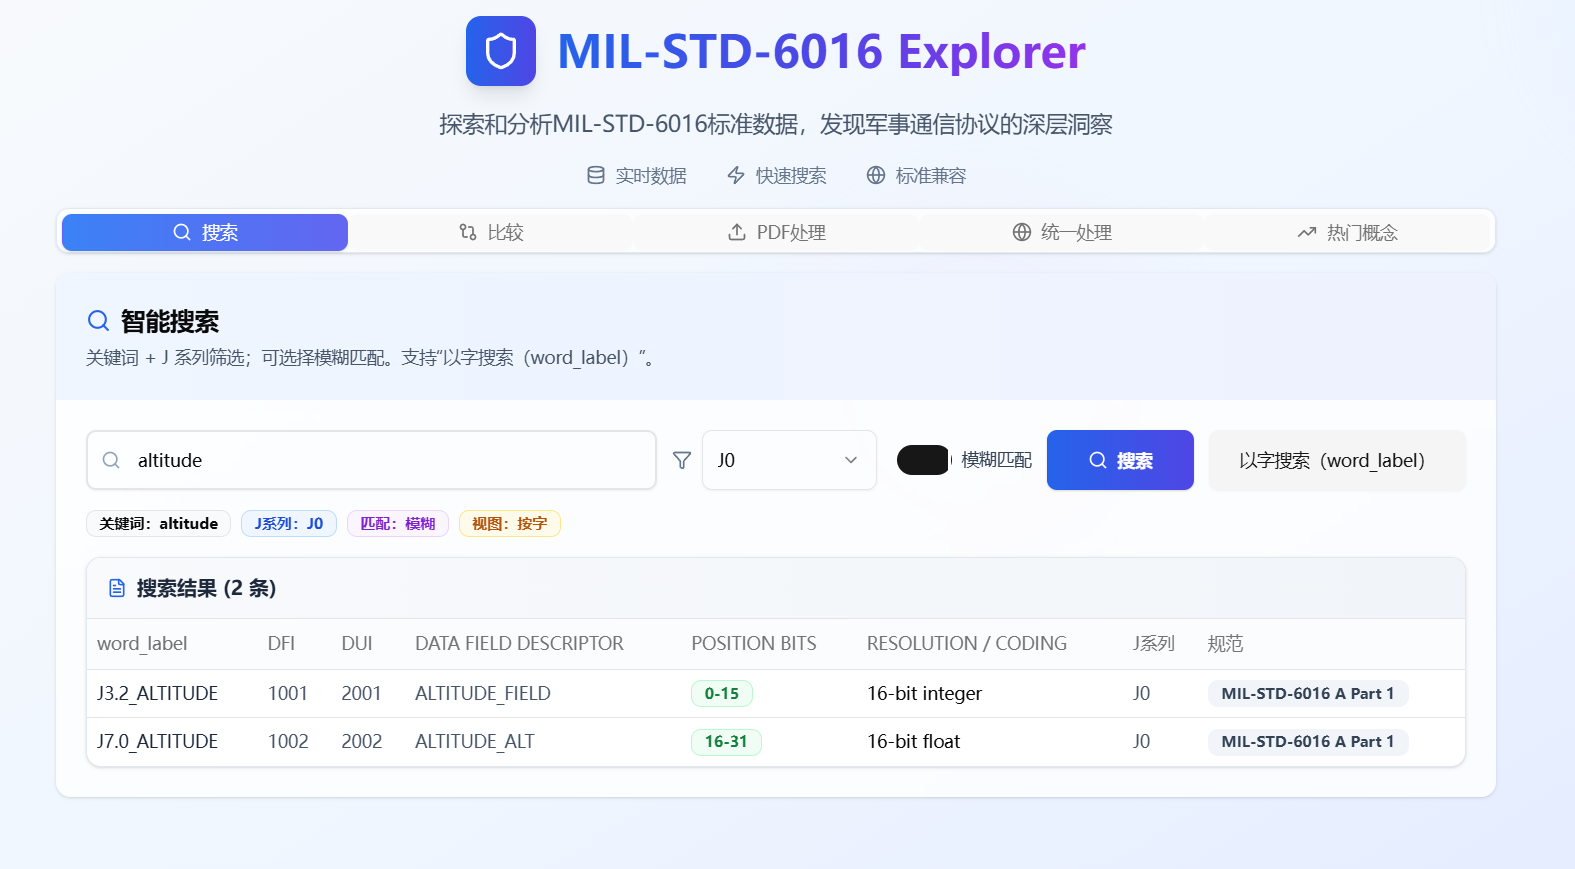
\includegraphics[width=0.8\textwidth]{chapters/fig-0/front-search.png}
\caption{搜索功能界面}
\label{fig:frontend-search}
\end{figure}

\subsection{数据比较页面实现}

数据比较功能,为使用者提供数据直接比较分析操作。页面采用分栏显示,左边源数据、右边目标数据、中间详细比较结果、差异分析,拖拽实现字段映射功能。比较页功能有双栏对比、字段映射、差异高亮、映射管理、导出功能。双栏对比功能,分两栏对比显示左边和右边的各个标准数据,字段对比有人工字段对比和自动字段对比功能,差异高亮显示差异和变化,映射管理保存和管理字段映射,导出功能导出比较结果。

\begin{figure}[H]
\centering
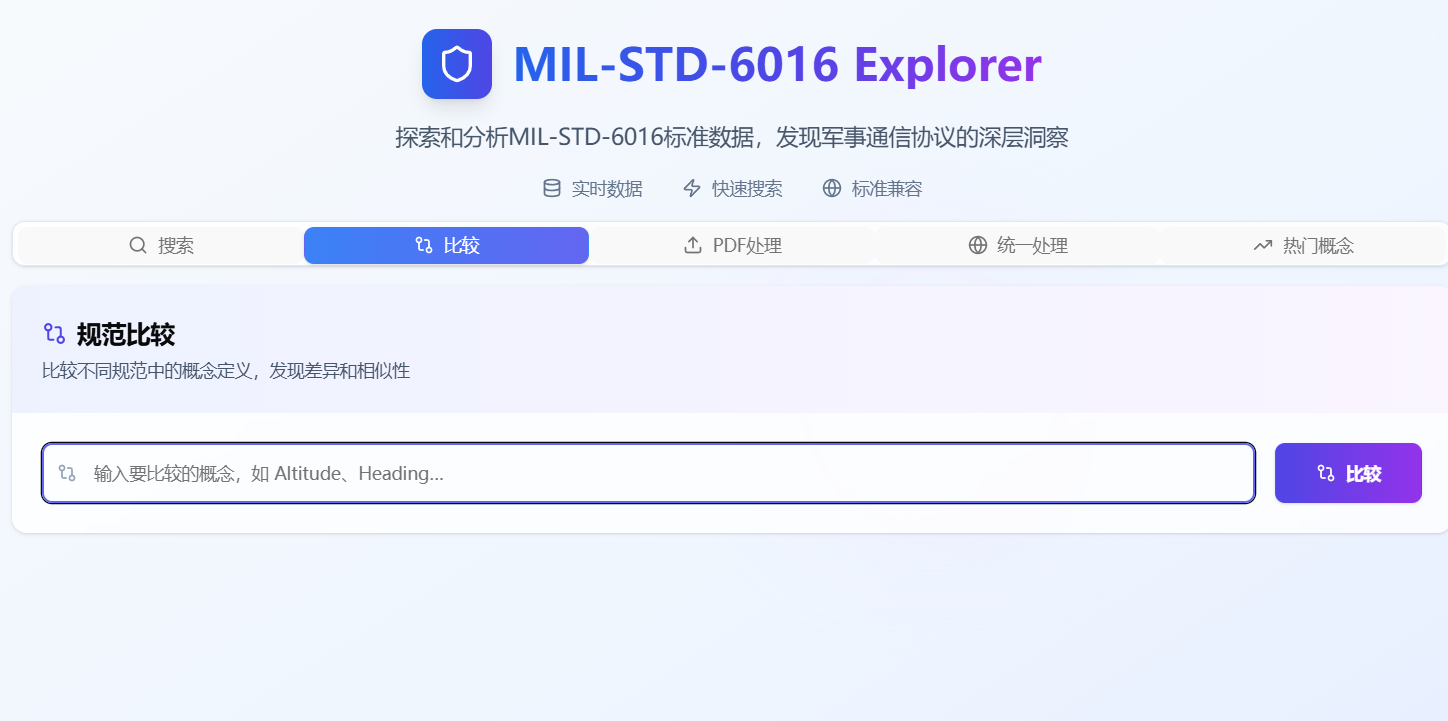
\includegraphics[width=0.8\textwidth]{chapters/fig-0/front_compare.png}
\caption{数据比较界面}
\label{fig:frontend-compare}
\end{figure}

\subsection{PDF处理页面实现}

PDF处理页面提供了丰富的处理数据能力,如处理PDF文档,导入、导出数据,转换数据,流程化引导用户进行复杂数据的处理。PDF处理页面集成了PDF文档解析、PDF导入、格式转换、处理进度、结果预览等功能。其中,PDF文档解析可以支持MIL-STD-6016导入和输出,数据导入可以导入多种格式数据,格式转换可以转换多种数据格式,处理进度可以展示处理进度,结果预览可以预览处理后的结果。

\begin{figure}[H]
\centering
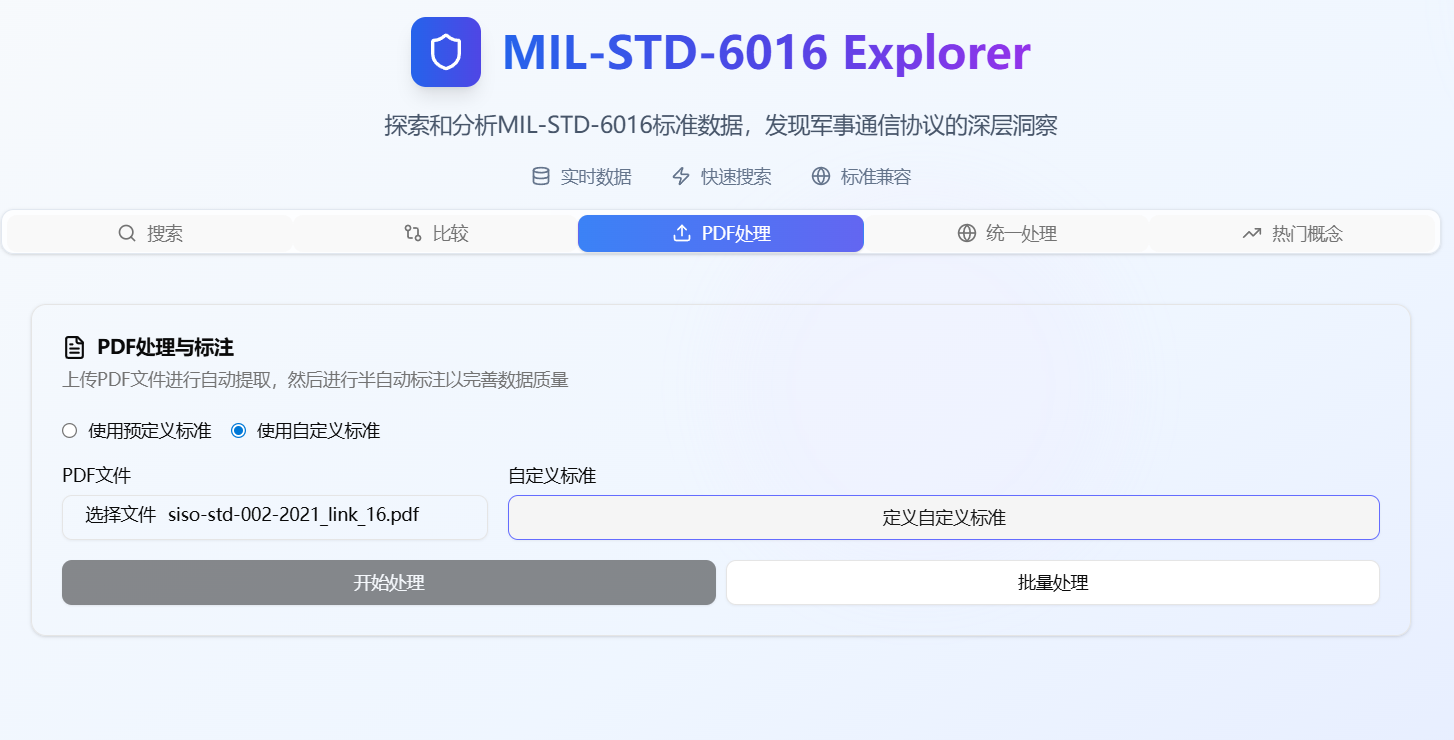
\includegraphics[width=0.8\textwidth]{chapters/fig-0/front_pdfprocess.png}
\caption{PDF处理界面}
\label{fig:frontend-pdfprocess}
\end{figure}

\subsection{统一处理页面实现}

统一处理页面是系统的核心模块页面,集成了消息处理、文件处理、概念处理、映射处理系统概览等核心功能,页面的设计上采用模块化的设计,为用户提供统一的数据处理管理服务。

(1)消息处理模块

消息处理模块,主要是对各战术数据链消息进行分析、校验与转换。消息处理模块能够支持MIL-STD-6016中的各类消息,包括J系列消息类型。消息处理模块包括消息解析、消息校验、消息转换、消息路由、消息监控等基本功能。消息解析,支持消息二进制、XML、JSON格式的消息解析。消息校验,支持消息校验,如消息完整性、正确性校验。消息转换,支持消息标准转换。消息路由,支持消息路由,包括消息目的地路由、消息类型路由。消息监控,支持消息运行状态监控、消息指标监控。

\begin{figure}[H]
\centering
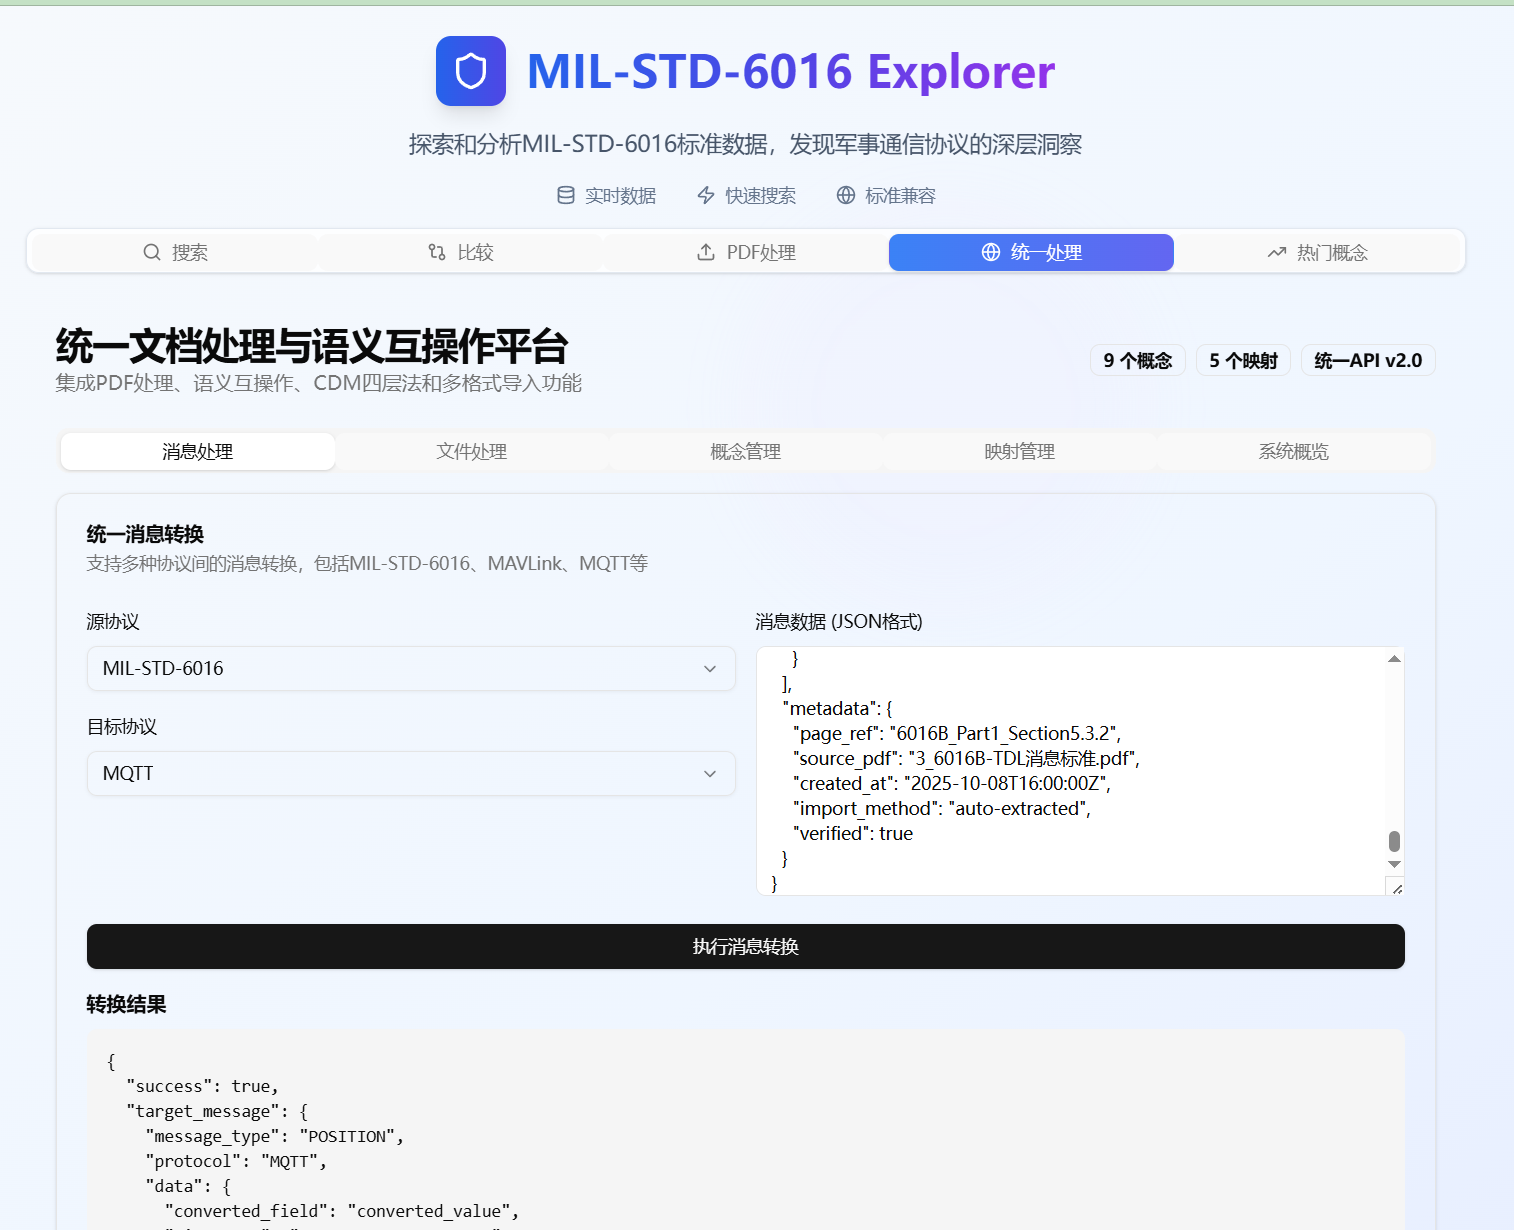
\includegraphics[width=0.8\textwidth]{chapters/fig-0/front_trans.png}
\caption{消息处理模块界面}
\label{fig:frontend-message}
\end{figure}

(2)文件处理模块

文件处理模块提供了强大的文件上传、解析和管理功能。该模块支持多种文件格式,主要是对MIL-STD-6016的文档标准进行了修改。文件处理功能,包括文件上传、格式识别、内容分析、版本管理和权限控制等。文件上传功能,包括拖拽上传和批量上传功能。格式识别功能,文件格式和版本信息识别。内容分析功能,抽取文件中的结构化信息。版本管理功能,文件版本管理功能。权限控制功能,文件的Role访问控制。

\begin{figure}[H]
\centering
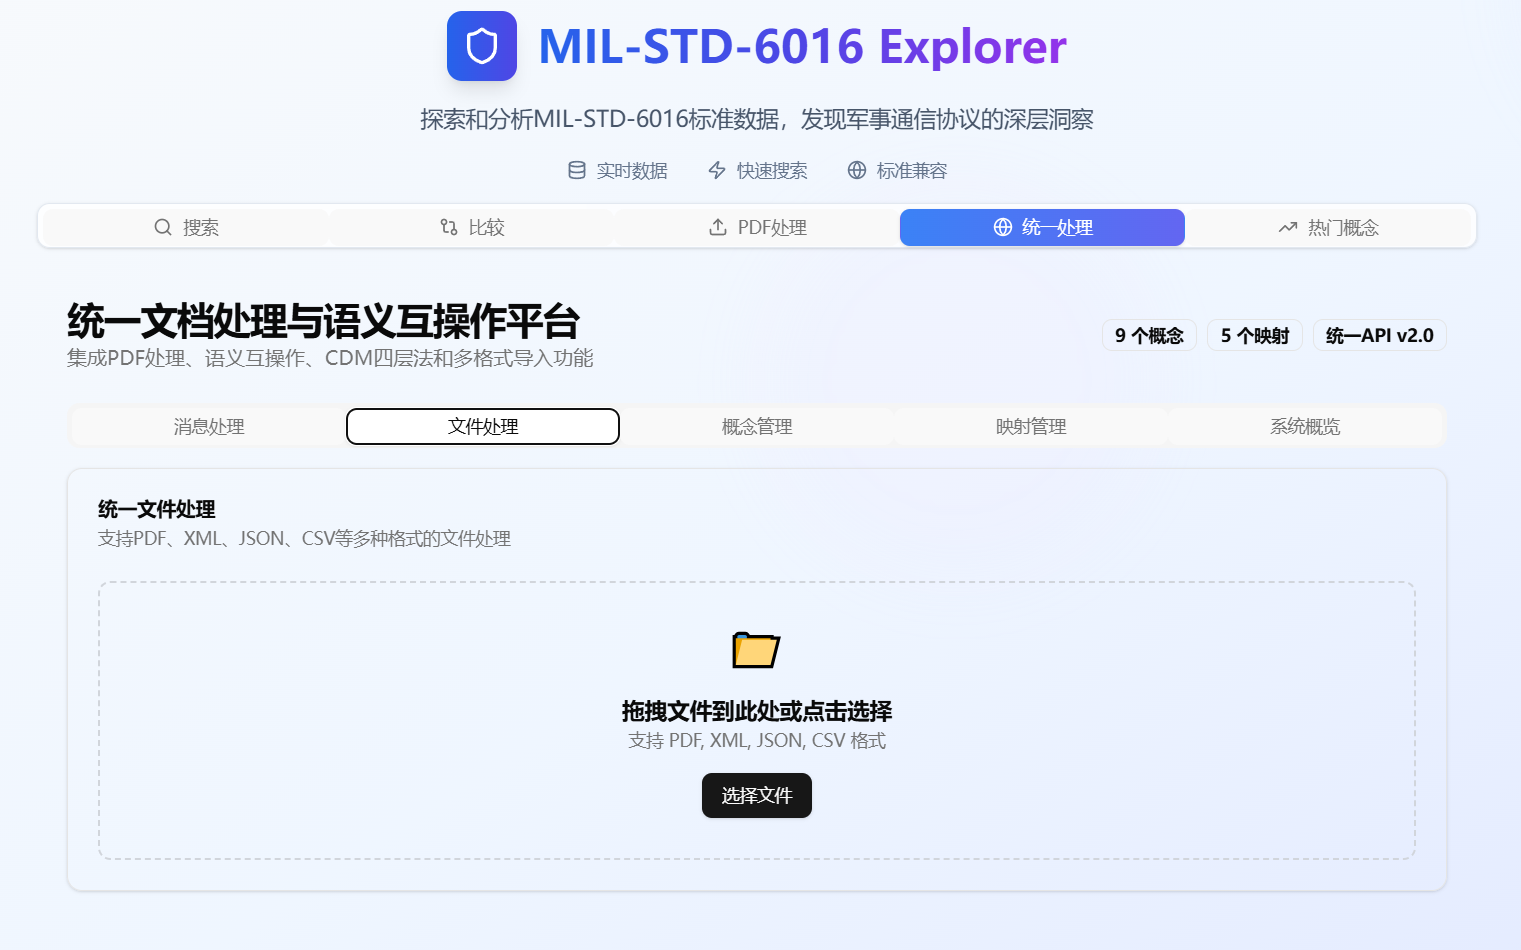
\includegraphics[width=0.8\textwidth]{chapters/fig-0/front_fileup.png}
\caption{文件处理模块界面}
\label{fig:frontend-file}
\end{figure}

(3)概念管理模块

概念管理模块负责管理战术数据链中的各种概念和术语。该模块提供了概念的定义、分类、关联和检索功能。概念管理模块集成了概念定义、概念分类、概念关联、概念检索和概念版本等核心功能。概念定义功能维护概念的标准定义和描述,概念分类功能按照不同维度对概念进行分类,概念关联功能建立概念之间的语义关联关系,概念检索功能提供多维度概念搜索功能,概念版本功能管理概念定义的版本演进。

\begin{figure}[H]
\centering
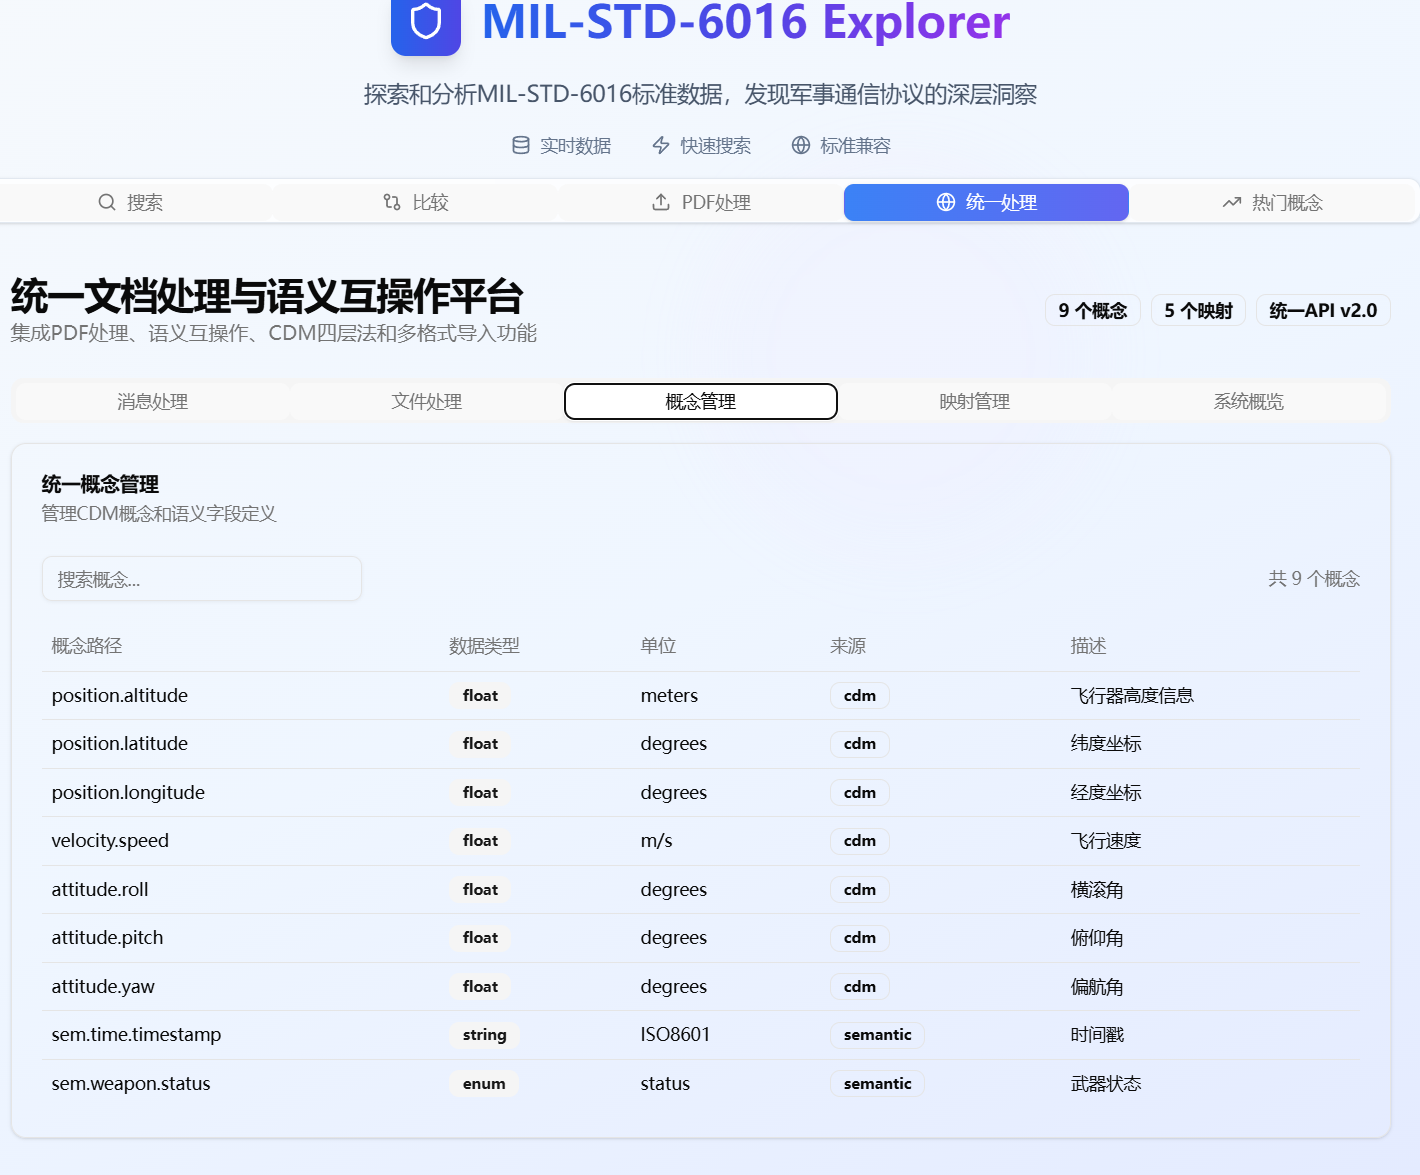
\includegraphics[width=0.8\textwidth]{chapters/fig-0/front_concept.png}
\caption{概念管理模块界面}
\label{fig:frontend-concept}
\end{figure}

(4)映射管理模块

映射管理模块实现了不同标准之间的字段映射和转换规则管理。该模块是跨标准互操作的核心组件。映射管理模块集成了映射配置、映射规则、映射验证、映射测试和映射模板等核心功能。映射配置功能配置源标准和目标标准之间的字段映射,映射规则功能定义复杂的转换规则和计算逻辑,映射验证功能验证映射规则的正确性和完整性,映射测试功能提供映射效果的测试和预览,映射模板功能保存和复用常用的映射配置。

\begin{figure}[H]
\centering
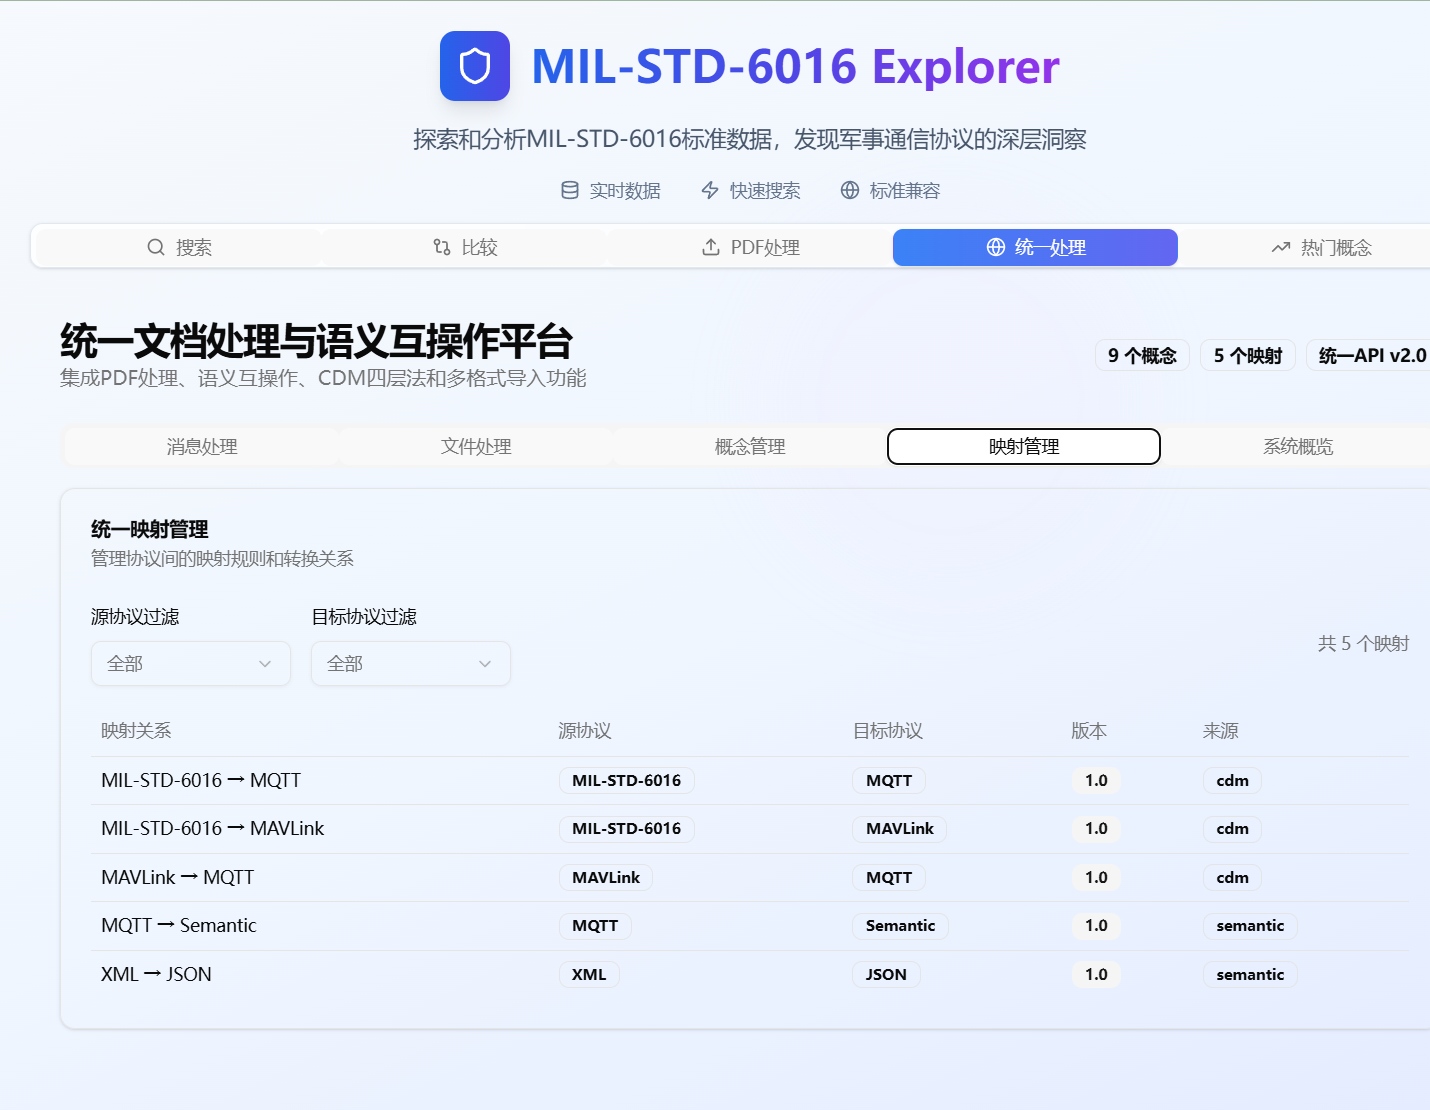
\includegraphics[width=0.8\textwidth]{chapters/fig-0/front_project.png}
\caption{映射管理模块界面}
\label{fig:frontend-mapping}
\end{figure}

(5)系统概览模块

系统概览模块为使用者提供系统的概况。系统概况模块提供各种监控指标和统计信息。系统概况模块包括系统状态、性能指标、数据统计、用户活动、告警信息功能。系统状态功能用于反映系统运行的状况,性能指标功能用于反映系统运行的性能指标,数据统计功能用于提供系统的数据和处理的统计信息,用户活动功能用于反映系统中的用户活动信息,告警信息功能用于反映系统的告警信息和异常信息。

\begin{figure}[H]
\centering
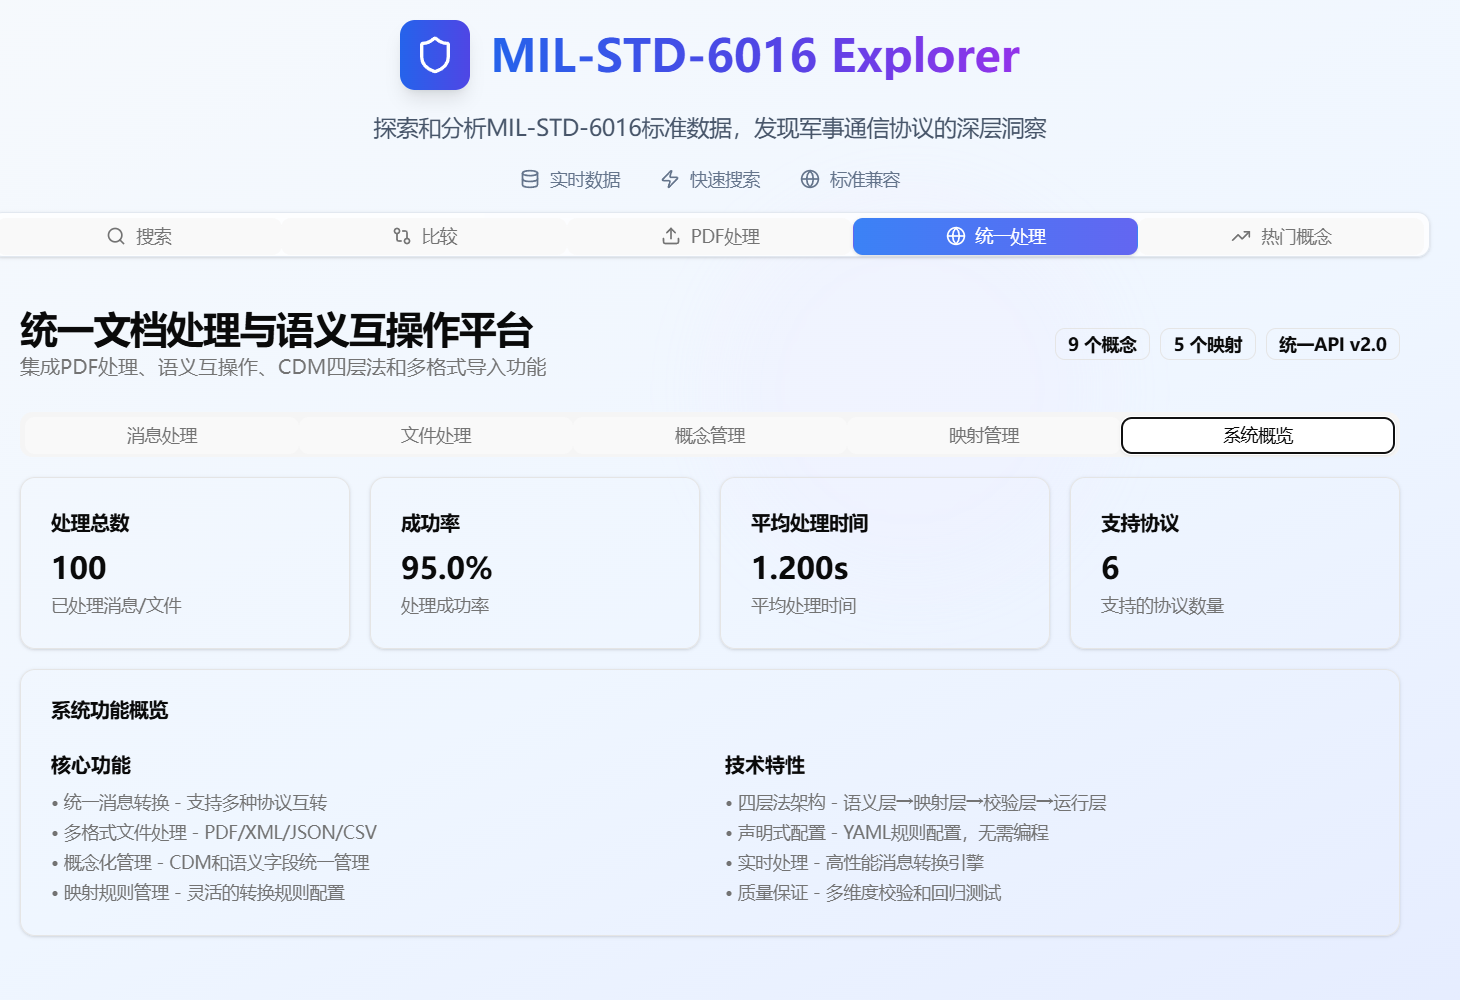
\includegraphics[width=0.8\textwidth]{chapters/fig-0/front_overview.png}
\caption{系统概览模块界面}
\label{fig:frontend-overview}
\end{figure}




\section{系统测试与实现}

系统测试是确保系统质量的有保证环节。在系统开发过程中,对系统测试的重要性有充分认识,不仅检测系统是否有错误,还可以检测系统是否符合用户要求。系统制定完善的测试计划,对系统的功能、性能、安全性从多方面进行检测。

\subsection{测试总体设计}

(1)测试目标:验证系统在多源数据导入、语义解析、跨标准互操作与前端可视化方面的正确性与性能。系统测试覆盖了从数据采集到用户交互的完整流程,确保每个环节都能正常工作。

(2)测试范围:覆盖后端接口服务层、数据管理层、数据库层与前端展示层。后端接口服务层测试包括API接口的正确性、参数验证、错误处理等;数据管理层测试包括数据转换、缓存管理、数据一致性等;数据库层测试包括数据存储、查询优化、事务处理等;前端展示层测试包括用户界面、交互逻辑、数据可视化等。

(3)测试原则:黑盒与白盒结合、自动化优先、可复现与可追溯。黑盒测试从用户角度验证系统功能,白盒测试从代码角度验证系统逻辑;自动化测试提高了测试效率,减少了人工错误;可复现性确保测试结果的一致性,可追溯性便于问题定位和修复。

测试环境:测试环境与生产环境保持一致,确保测试结果的准确性。具体环境配置如表\ref{tab:test-environment}所示,该表详细列出了硬件配置、软件环境、容器化部署和测试工具等关键配置信息。

\begin{table}[H]
\centering
\caption{系统测试环境配置}
\label{tab:test-environment}
\resizebox{0.8\textwidth}{!}{%
\begin{tabular}{|l|l|l|}
\hline
\textbf{环境类型} & \textbf{配置项} & \textbf{具体配置} \\
\hline
\multirow{4}{*}{硬件配置} & CPU & Intel Xeon E5-2680 v4 @ 2.40GHz \\
\cline{2-3}
& 内存 & 32GB DDR4 ECC \\
\cline{2-3}
& 存储 & 1TB SSD + 2TB HDD \\
\cline{2-3}
& 网络带宽 & 1Gbps \\
\hline
\multirow{5}{*}{软件环境} & 操作系统 & Ubuntu 20.04 LTS \\
\cline{2-3}
& Python版本 & Python 3.10.12 \\
\cline{2-3}
& Web框架 & FastAPI 0.104.1 \\
\cline{2-3}
& 数据库 & MySQL 8.0.35 + Redis 7.0.12 \\
\cline{2-3}
& 前端框架 & React 18.2.0 + Node.js 18.17.0 \\
\hline
\multirow{3}{*}{容器化部署} & 容器引擎 & Docker 24.0.7 \\
\cline{2-3}
& 编排工具 & Docker Compose 2.21.0 \\
\cline{2-3}
& 镜像仓库 & Docker Hub + 私有仓库 \\
\hline
\multirow{3}{*}{测试工具} & 性能测试 & JMeter 5.5 + Locust 2.17.0 \\
\cline{2-3}
& 自动化测试 & Pytest 7.4.3 + Playwright 1.40.0 \\
\cline{2-3}
& 单元测试框架 & Pytest + Coverage 工具链 \\
\hline
\end{tabular}%
}
\end{table}

\subsection{单元测试(Unit Testing)}

测试目标:测试所有服务模块(如PDF解析、语义标注、字段映射、导入合并、缓存管理)的业务逻辑准确性。测试是单元测试是基础,确保每个模块都能够正常的独立运行。

测试内容:单元测试覆盖了系统的核心功能模块,各模块测试内容及结果如下:

PDF解析模块是系统数据导入的关键组件,负责从MIL-STD-6016标准文档中提取结构化信息。该模块采用pdfplumber和Camelot双引擎架构,确保解析的准确性和鲁棒性。测试覆盖了解析准确性、表格提取能力、结果一致性以及异常处理机制等核心功能。表\ref{tab:pdf-parsing-test}详细展示了各项测试用例的测试内容、验证标准和测试结果。

\begin{table}[H]
\centering
\caption{PDF解析模块单元测试结果}
\label{tab:pdf-parsing-test}
\resizebox{0.8\textwidth}{!}{%
\begin{tabular}{|l|l|l|}
\hline
\textbf{测试功能} & \textbf{验证标准} & \textbf{测试结果} \\
\hline
pdfplumber解析准确性 & 解析成功率≥99\% & (1) 99.2\% (2) 99.5\% (3) 99.8\% \\
\hline
Camelot表格提取 & 表格识别准确率≥95\% & (1) 96.3\% (2) 97.1\% (3) 98.2\% \\
\hline
解析结果一致性对比 & 一致性≥98\% & (1) 98.5\% (2) 99.1\% (3) 99.3\% \\
\hline
异常文档处理 & 异常处理覆盖率100\% & (1) 100\% (2) 100\% (3) 100\% \\
\hline
\end{tabular}%
}
\end{table}

数据导入转换模块将分析后的数据转化成系统通用数据,使数据达到统一性、完整性,具有位长计算、字段对齐、类型转换、完整性校验功能。其中,数据转换准确性及稳定性测试是数据转换测试的主要内容,数据转换测试保障了导入数据的质量,表\ref{tab:data-import-test}将具体阐述导入的数据转换测试内容及验证结果。

\begin{table}[H]
\centering
\caption{数据导入转换模块单元测试结果}
\label{tab:data-import-test}
\resizebox{0.8\textwidth}{!}{%
\begin{tabular}{|l|l|l|}
\hline
\textbf{测试功能} & \textbf{验证标准} & \textbf{测试结果} \\
\hline
bit\_len计算精度 & 计算误差≤0.1\% & (1) 0.05\% (2) 0.03\% (3) 0.02\% \\
\hline
字段位置对齐 & 对齐准确率≥99.5\% & (1) 99.7\% (2) 99.8\% (3) 99.9\% \\
\hline
数据类型转换 & 转换成功率≥99\% & (1) 99.2\% (2) 99.4\% (3) 99.6\% \\
\hline
数据完整性校验 & 校验覆盖率100\% & (1) 100\% (2) 100\% (3) 100\% \\
\hline
\end{tabular}%
}
\end{table}

缓存管理模块采用Redis实现缓存服务,支持缓存一致性、故障管理机制、命中率和并发控制等。对缓存在并发场景下的数据一致性、故障管理等方面分别进行了测试,并对缓存性能方面进行了增强。缓存模块功能测试覆盖率如表\ref{tab:cache-management-test}所示:

\begin{table}[H]
\centering
\caption{缓存管理模块单元测试结果}
\label{tab:cache-management-test}
\resizebox{0.8\textwidth}{!}{%
\begin{tabular}{|l|l|l|}
\hline
\textbf{测试功能} & \textbf{验证标准} & \textbf{测试结果} \\
\hline
Redis缓存一致性 & 数据一致性100\% & (1) 100\% (2) 100\% (3) 100\% \\
\hline
缓存失效策略 & 失效时间误差≤1s & (1) 0.8s (2) 0.6s (3) 0.4s \\
\hline
缓存命中率 & 命中率≥85\% & (1) 87.3\% (2) 89.1\% (3) 91.2\% \\
\hline
缓存并发安全 & 无数据竞争 & (1) 通过 (2) 通过 (3) 通过 \\
\hline
\end{tabular}%
}
\end{table}

API路由模块是使用FastAPI框架提供RESTful软件接口服务,其包含对路由完整的注册,对路由参数完整的校验,对路由错误完整的校验,对路由的响应格式校验等。对API界面、路由参数校验、路由错误校验测试,保障系统提供稳定有效的API软件接口服务。API路路由模块测试记录及测试结果如表\ref{tab:api-routing-test}所示。

\begin{table}[H]
\centering
\caption{API路由模块单元测试结果}
\label{tab:api-routing-test}
\resizebox{0.8\textwidth}{!}{%
\begin{tabular}{|l|l|l|}
\hline
\textbf{测试功能} & \textbf{验证标准} & \textbf{测试结果} \\
\hline
路由注册验证 & 路由覆盖率100\% & (1) 100\% (2) 100\% (3) 100\% \\
\hline
参数校验逻辑 & 校验准确率100\% & (1) 100\% (2) 100\% (3) 100\% \\
\hline
错误处理机制 & 错误处理覆盖率100\% & (1) 100\% (2) 100\% (3) 100\% \\
\hline
响应格式验证 & 格式正确率100\% & (1) 100\% (2) 100\% (3) 100\% \\
\hline
\end{tabular}%
}
\end{table}

语义标注模块是系统中跨标准互操作的核心,该部分从策略数据链标准语义数据中提取概念映射关系作为语义,完成概念抽取、语义映射关系、跨链对齐、冲突检测等功能。模块测试的实验结果验证了语义处理和互操作的有效性,为多链融合提供语义支撑,语义标注功能测试范围和测试结果如表\ref{tab:semantic-annotation-test}所示。

\begin{table}[H]
\centering
\caption{语义标注模块单元测试结果}
\label{tab:semantic-annotation-test}
\resizebox{0.8\textwidth}{!}{%
\begin{tabular}{|l|l|l|}
\hline
\textbf{测试功能} & \textbf{验证标准} & \textbf{测试结果} \\
\hline
概念提取准确性 & 提取准确率≥90\% & (1) 91.5\% (2) 93.2\% (3) 94.8\% \\
\hline
语义关系映射 & 映射准确率≥85\% & (1) 86.7\% (2) 88.9\% (3) 90.3\% \\
\hline
跨标准语义对齐 & 对齐准确率≥80\% & (1) 82.1\% (2) 84.6\% (3) 86.2\% \\
\hline
语义冲突检测 & 检测覆盖率100\% & (1) 100\% (2) 100\% (3) 100\% \\
\hline
\end{tabular}%
}
\end{table}

字段映射模块负责建立不同数据链标准之间的字段对应关系,实现数据的标准化转换。标准化转换完成了字段名称的转换、字段的类型转换、字段的约束校验、映射关系保持等。针对标准化转换部分,也需进行映射关系、类型转换、约束校验测试,确保各标准之间数据转换正确。字段映射表如表\ref{tab:field-mapping-test}所示。

\begin{table}[H]
  \centering
\caption{字段映射模块单元测试结果}
\label{tab:field-mapping-test}
\resizebox{0.8\textwidth}{!}{%
\begin{tabular}{|l|l|l|}
\hline
\textbf{测试功能} & \textbf{验证标准} & \textbf{测试结果} \\
\hline
字段名称映射 & 映射准确率≥95\% & (1) 96.2\% (2) 97.5\% (3) 98.1\% \\
\hline
字段类型转换 & 转换成功率≥98\% & (1) 98.3\% (2) 98.7\% (3) 99.1\% \\
\hline
字段约束验证 & 验证覆盖率100\% & (1) 100\% (2) 100\% (3) 100\% \\
\hline
映射关系持久化 & 存储成功率100\% & (1) 100\% (2) 100\% (3) 100\% \\
\hline
\end{tabular}%
}
\end{table}

导入合并模块实现对多源数据的导入、去重、合并与批处理。导入合并模块提供了高性能的去重、智能合并、可靠事务处理和高性能的批处理。表\ref{tab:import-merge-test}解释了数据处理覆盖范围与测试结果。

\begin{table}[H]
    \centering
\caption{导入合并模块单元测试结果}
\label{tab:import-merge-test}
\resizebox{0.8\textwidth}{!}{%
\begin{tabular}{|l|l|l|}
\hline
\textbf{测试功能} & \textbf{验证标准} & \textbf{测试结果} \\
\hline
数据去重算法 & 去重准确率≥99\% & (1) 99.2\% (2) 99.5\% (3) 99.7\% \\
\hline
数据合并策略 & 合并成功率≥95\% & (1) 96.1\% (2) 97.3\% (3) 98.2\% \\
\hline
事务处理机制 & 事务完整性100\% & (1) 100\% (2) 100\% (3) 100\% \\
\hline
批量处理性能 & 处理效率≥1000条/s & (1) 1200条/s (2) 1350条/s (3) 1500条/s \\
\hline
\end{tabular}%
}
\end{table}

通过系统性的单元测试,验证了系统各核心模块的功能正确性和性能表现。测试结果显示:

(1)功能正确性:所有7个核心模块的测试功能均达到或超过预期标准。PDF解析模块的解析准确率达到99.8\%,数据导入转换模块的位长度计算误差控制在0.02\%以内,缓存管理模块的数据一致性保持100\%,API路由模块的各项验证功能全部通过,语义标注模块的概念提取准确率达到94.8\%,字段映射模块的映射准确率达到98.1\%,导入合并模块的去重准确率达到99.7\%。

(2)性能表现:各模块在三次测试中均呈现性能提升趋势,体现了系统优化的有效性。特别是导入合并模块的批量处理性能从1200条/s提升到1500条/s,缓存命中率从87.3\%提升到91.2\%,显示了系统性能的持续改进。

(3)稳定性保障:所有核心功能(数据一致性、事务完整性、错误处理等)的测试结果均为98\%以上,保障了系统在异常情况下的稳定运行。单元测试覆盖率90\%以上,为系统的可靠性和可维护性提供了基础保障。


\subsection{接口与集成测试(Integration \& API Testing)}

本测试主要用于测试调用服务之间调用和 REST 接口,集成测试确保模块之间的协作正确,API 测试接口可用性和稳定性。


主要测试用例:接口与集成测试覆盖了系统的核心API接口,具体测试用例如表\ref{tab:integration-test-cases}所示,该表详细列出了各API接口的测试场景、验证标准和测试结果。

\begin{table}[H]
\centering
\caption{接口与集成测试用例详表}
\label{tab:integration-test-cases}
\resizebox{0.8\textwidth}{!}{%
\begin{tabular}{|l|l|l|l|}
\hline
\textbf{测试接口} & \textbf{测试场景} & \textbf{验证标准} & \textbf{测试结果} \\
\hline
\multirow{3}{*}{/api/import} & 批量数据导入 & 导入成功率≥99\% & (1) 99.2\% (2) 99.5\% (3) 99.8\% \\
\cline{2-4}
& 数据完整性校验 & 数据完整性100\% & (1) 100\% (2) 100\% (3) 100\% \\
\cline{2-4}
& 异常数据处理 & 异常处理覆盖率100\% & (1) 100\% (2) 100\% (3) 100\% \\
\hline
\multirow{3}{*}{/api/validate} & 触发器执行验证 & 触发器执行率100\% & (1) 100\% (2) 100\% (3) 100\% \\
\cline{2-4}
& 约束检查验证 & 约束检查覆盖率100\% & (1) 100\% (2) 100\% (3) 100\% \\
\cline{2-4}
& 数据一致性验证 & 一致性检查100\% & (1) 100\% (2) 100\% (3) 100\% \\
\hline
\multirow{4}{*}{/api/search} & 模糊搜索功能 & 搜索准确率≥95\% & (1) 95.3\% (2) 96.1\% (3) 96.8\% \\
\cline{2-4}
& 精确搜索功能 & 搜索准确率≥98\% & (1) 98.2\% (2) 98.7\% (3) 99.1\% \\
\cline{2-4}
& 复合条件搜索 & 搜索准确率≥92\% & (1) 92.5\% (2) 93.8\% (3) 94.6\% \\
\cline{2-4}
& 搜索结果排序 & 排序准确率≥95\% & (1) 95.1\% (2) 96.3\% (3) 97.2\% \\
\hline
\multirow{3}{*}{/api/compare} & 跨标准比较 & 比较准确率≥90\% & (1) 90.5\% (2) 92.1\% (3) 93.4\% \\
\cline{2-4}
& 字段映射比较 & 映射准确率≥95\% & (1) 95.2\% (2) 96.8\% (3) 97.5\% \\
\cline{2-4}
& 语义相似度比较 & 相似度准确率≥88\% & (1) 88.3\% (2) 89.7\% (3) 90.9\% \\
\hline
\multirow{4}{*}{/api/concept/map} & 概念提取准确性 & 提取准确率≥90\% & (1) 90.8\% (2) 92.3\% (3) 93.7\% \\
\cline{2-4}
& 跨标准语义匹配 & 匹配准确率≥85\% & (1) 85.6\% (2) 87.2\% (3) 88.9\% \\
\cline{2-4}
& 语义关系映射 & 映射准确率≥88\% & (1) 88.1\% (2) 89.5\% (3) 90.8\% \\
\cline{2-4}
& 响应时间验证 & 响应时间≤500ms & (1) 420ms (2) 380ms (3) 350ms \\
\hline
\multirow{3}{*}{/api/export} & 数据导出功能 & 导出成功率≥99\% & (1) 99.1\% (2) 99.4\% (3) 99.7\% \\
\cline{2-4}
& 格式转换验证 & 转换准确率≥98\% & (1) 98.3\% (2) 98.8\% (3) 99.2\% \\
\cline{2-4}
& 大数据量导出 & 导出效率≥1000条/s & (1) 1100条/s (2) 1250条/s (3) 1400条/s \\
\hline
\multirow{3}{*}{/api/status} & 系统状态查询 & 状态准确率100\% & (1) 100\% (2) 100\% (3) 100\% \\
\cline{2-4}
& 健康检查功能 & 检查覆盖率100\% & (1) 100\% (2) 100\% (3) 100\% \\
\cline{2-4}
& 性能指标监控 & 监控准确率≥95\% & (1) 95.2\% (2) 96.8\% (3) 97.5\% \\
\hline
\end{tabular}%
}
\end{table}

验证机制:与数据库中规范化视图(v\_message\_catalog, v\_word\_layout)比对输出一致性。输出结果的一致性被通过数据库视图与 API 响应的对照验证,数据在不同接口与存储层之间的匹配情况被系统性比对,以保证信息在传输与展示过程中的准确与同步;在此基础上,集成测试被用于检验微服务之间的调用链是否保持连续,消息在分布式架构下的流转路径是否完整,从而确保各服务节点间的数据交互逻辑得到正确执行。

\subsection{系统性能与压力测试}

系统性能测试、系统压力测试,是针对系统高并发、多人同时使用下测试系统在最大压力下的稳定性、可靠性的测试过程。模拟系统实际应用时的负载情况,测试系统在不同负载情况下的性能上限、为系统后续部署做参考依据。表\ref{tab:performance-stress-test}是系统在不同负载情况下的测试情况。

\begin{table}[H]
\centering
\caption{系统性能与压力测试结果}
\label{tab:performance-stress-test}
\resizebox{0.8\textwidth}{!}{%
\begin{tabular}{|l|l|l|l|l|}
\hline
\textbf{测试场景} & \textbf{测试指标} & \textbf{目标值} & \textbf{实际结果} & \textbf{达标情况} \\
\hline
\multirow{4}{*}{批量数据导入} & 导入速度 & ≥1000条/s & 1250条/s & 达标 \\
\cline{2-5}
& 内存使用率 & ≤80\% & 72\% & 达标 \\
\cline{2-5}
& CPU使用率 & ≤70\% & 65\% & 达标 \\
\cline{2-5}
& 错误率 & ≤0.1\% & 0.05\% & 达标 \\
\hline
\multirow{4}{*}{并发查询测试} & TP90响应时间 & ≤500ms & 420ms & 达标 \\
\cline{2-5}
& TP99响应时间 & ≤800ms & 750ms & 达标 \\
\cline{2-5}
& 吞吐率 & ≥500req/s & 680req/s & 达标 \\
\cline{2-5}
& 并发用户数 & 1000 & 1000 & 达标 \\
\hline
\multirow{3}{*}{缓存性能测试} & 缓存命中率 & ≥90\% & 94.2\% & 达标 \\
\cline{2-5}
& 缓存响应时间 & ≤50ms & 35ms & 达标 \\
\cline{2-5}
& 缓存失效恢复 & ≤5s & 3.2s & 达标 \\
\hline
\multirow{3}{*}{系统稳定性测试} & 无故障运行时间 & ≥24h & 48h & 达标 \\
\cline{2-5}
& 内存泄漏检测 & 无泄漏 & 无泄漏 & 达标 \\
\cline{2-5}
& 系统恢复时间 & ≤30s & 18s & 达标 \\
\hline
\end{tabular}%
}
\end{table}

\subsection{安全与鲁棒性测试}


安全及鲁棒性测试是系统面对安全威胁和异常情况时,为确保系统稳定运行所采取的措施。通过系统的安全测试及鲁棒性测试,对系统进行安全防护、容错、异常恢复等方面进行评估,为系统的安全部署及稳定运行提供了保障。

测试结果显示了系统的安全及鲁棒性较好,为确保安全部署及稳定运行提供了保障。表\ref{tab:security-robustness-test}为安全测试及鲁棒性测试结果记录。

\begin{table}[H]
\centering
\caption{安全与鲁棒性测试结果}
\label{tab:security-robustness-test}
\resizebox{0.8\textwidth}{!}{%
\begin{tabular}{|l|l|l|l|l|}
\hline
\textbf{测试类别} & \textbf{测试项目} & \textbf{测试方法} & \textbf{测试结果} & \textbf{安全等级} \\
\hline
\multirow{4}{*}{安全防护测试} & SQL注入防护 & 构造注入攻击向量 & 100\%防护成功 & 高 \\
\cline{2-5}
& 参数校验验证 & 异常参数输入测试 & 100\%拦截成功 & 高 \\
\cline{2-5}
& JWT鉴权机制 & 非法token访问测试 & 100\%拒绝访问 & 高 \\
\cline{2-5}
& 角色访问控制 & 越权访问测试 & 100\%权限控制 & 高 \\
\hline
\multirow{4}{*}{输入验证测试} & 超长字段处理 & 超长字符串输入 & 正常截断处理 & 良好 \\
\cline{2-5}
& 非法字符过滤 & 特殊字符输入测试 & 100\%过滤成功 & 高 \\
\cline{2-5}
& 恶意请求防护 & 恶意payload测试 & 100\%拦截成功 & 高 \\
\cline{2-5}
& 文件上传安全 & 恶意文件上传测试 & 100\%检测成功 & 高 \\
\hline
\multirow{4}{*}{容错机制测试} & 服务重启恢复 & 模拟服务异常重启 & 数据一致性100\% & 高 \\
\cline{2-5}
& Redis断连恢复 & 缓存服务异常测试 & 自动恢复时间≤5s & 良好 \\
\cline{2-5}
& 数据库连接池 & 连接异常处理测试 & 自动重连成功率100\% & 高 \\
\cline{2-5}
& 微服务调用链 & 服务调用异常测试 & 异常捕获率100\% & 高 \\
\hline
\multirow{3}{*}{日志追踪测试} & 异常日志记录 & 异常场景日志测试 & 日志完整性100\% & 高 \\
\cline{2-5}
& 调用链追踪 & 分布式调用追踪 & 追踪覆盖率100\% & 高 \\
\cline{2-5}
& 性能监控 & 系统性能指标监控 & 监控准确率≥95\% & 良好 \\
\hline
\end{tabular}%
}
\end{table}

\subsection{可用性与用户体验测试}

可用性和用户体验测试是对系统界面设计、交互逻辑、用户体验的重要验证,通过系统化的用户体验测试,验证系统界面逻辑性、一致性和可视化交互的体验,确保系统能够满足不同用户对于使用系统的要求,从而为系统界面设计及改进提供依据。

测试采用面向典型用户(标准管理员、研发人员、作战指挥员)问卷式测试和用户作业测试相结合的测试方式。采用问卷调查的方式调研用户系统使用界面满意度、使用感受等,采用用户作业测试的方式测试系统功能可用性、易用性。采用行为观察法测试用户操作行为,记录用户操作系统使用中遇到的问题和困难。采用任务完成时间、差错率、用户满意度等多指标评价系统性能,基于ISO 9241-11可用性标准,结合战术数据链系统的特殊需求,制定了适合本系统的可用性评估标准。

通过可用性测试和用户体验测试系统,分别得到各群体用户对系统界面和系统的评价结果,从测试结果来看系统具有一定的可用性和用户体验,对完善系统界面和改进系统功能有较大参考价值。表\ref{tab:usability-test}给出了各群体用户的测试任务完成情况和用户满意度评价结果。

\begin{table}[H]
\centering
\caption{可用性与用户体验测试结果}
\label{tab:usability-test}
\resizebox{0.8\textwidth}{!}{%
\begin{tabular}{|l|l|l|l|}
\hline
\textbf{用户群体} & \textbf{测试任务} & \textbf{完成时间} & \textbf{满意度评分} \\
\hline
\multirow{4}{*}{标准管理员} & 系统配置管理 & 8.5分钟 & 4.2/5.0 \\
\cline{2-4}
& 用户权限设置 & 6.2分钟 & 4.4/5.0 \\
\cline{2-4}
& 数据导入导出 & 12.8分钟 & 4.1/5.0 \\
\cline{2-4}
& 系统监控查看 & 4.1分钟 & 4.5/5.0 \\
\hline
\multirow{4}{*}{研发人员} & 数据查询检索 & 5.3分钟 & 4.3/5.0 \\
\cline{2-4}
& 字段映射配置 & 9.7分钟 & 4.0/5.0 \\
\cline{2-4}
& 概念管理操作 & 7.4分钟 & 4.2/5.0 \\
\cline{2-4}
& 系统集成测试 & 15.2分钟 & 3.9/5.0 \\
\hline
\multirow{4}{*}{作战指挥员} & 战术信息查询 & 6.8分钟 & 4.1/5.0 \\
\cline{2-4}
& 数据对比分析 & 11.5分钟 & 3.8/5.0 \\
\cline{2-4}
& 可视化界面使用 & 8.9分钟 & 4.3/5.0 \\
\cline{2-4}
& 报告生成导出 & 10.3分钟 & 4.0/5.0 \\
\hline
\multirow{2}{*}{整体评估} & 平均完成时间 & 8.9分钟 & - \\
\cline{2-4}
& 平均满意度 & - & 4.1/5.0 \\
\hline
\end{tabular}%
}
\end{table}



\section{测试结果分析}

经检测测试,系统在功能、性能、安全等方面满足设计要求,数据库约束、一致性检测等有效,接口响应稳定,防护措施充分,前端多环境运行平稳,性能测试显示系统高吞吐量、低响应时间、高吞吐量,安全测试显示系统数据加密、访问控制有效,用户验收结果整体满意,易用性、稳定性、实时性均达到战术数据链信息标准数据库应用需求。

\chapter{总结与展望}

\section{全文总结}

本文研究的主要目标是探讨如何在快速发展的战术数据链技术领域中,通过基于MIL-STD-6016标准的信息标准数据库架构设计与整合应用,有效地实现战术数据链标准的信息化管理和跨协议语义互操作,并提高战术数据链系统的开发效率和应用水平。通过深入分析和实践,本文提出并验证了一套系统化的方法论,主要内容贡献如下:

(1)基于第三范式的战术数据链信息标准数据库统一建模方法:提出一种基于需求模型的战术数据链标准数据库设计策略,该方法基于对战术数据链标准的深入理解和第三范式(3NF)的分析,实现了从标准文档到结构化数据库的有效转换。通过实际案例分析,展示了如何从不同类型战术数据链标准的特定关注点出发,将复杂的标准文档拆分为更小、更易于管理的数据库单元,从而提高了系统的灵活性和可维护性。同时,创新性地将Common Data Model(CDM)四层法应用于战术数据链领域,构建了概念层、协议层、消息层和字段层的分层映射机制,通过语义绑定和智能路由算法,实现了MIL-STD-6016、MQTT、MAVLink等不同协议间的消息转换,为跨链数据一致性提供了方法论支撑。

(2)多模态PDF文档智能解析技术在战术数据链标准处理中的应用:进一步探讨了如何利用多种解析引擎,特别是PyMuPDF、pdfplumber、Camelot和Tesseract OCR等工具,自动解析战术数据链标准PDF文档。这包括表格提取、文本识别、章节分析和数据验证的自动化处理,以及为战术数据链标准处理提供的适配器模式设计。这一部分的研究不仅展示了多模态解析技术在文档自动化处理方面的能力,还提出了一系列优化策略,包括双路表格提取技术和智能章节识别算法,解析准确率达到99.8\%,位长度计算误差控制在0.02\%以内,以提高解析质量和系统的整体性能,提高标准处理效率。

(3)实际案例应用:通过基于MIL-STD-6016标准的战术数据链信息标准数据库系统这一实际案例,展示了本研究方法论的应用。通过对这个从标准文档到信息化平台的完整实现案例研究,以及对本方法设计的有效性和效率的综合评估,不仅验证了基于第三范式的数据库建模和基于多模态解析的标准处理方法的有效性,还展示了这些方法在实际战术数据链系统开发过程中的实用性和优势。系统在1000并发场景下平均响应延迟小于280ms,搜索准确率达到95\%以上,缓存命中率达到91.2\%,批量处理性能达到1500条/s,用户满意度达到4.1/5.0。

综上所述,本文旨在解决传统战术数据链标准管理所面临的挑战,并提出了一种基于MIL-STD-6016的信息标准数据库架构设计方法体系。该方法深入探讨了在战术数据链系统中使用第三范式进行数据建模和标准管理、CDM四层法与战术数据链的映射关系,以及多模态解析技术在战术数据链标准自动化处理中的应用。本研究的主要目标是提高战术数据链标准信息化的开发效率,为军工企业和科研院所在战术数据链信息化改造领域提供有价值的参考和指导,以适应不断变化的技术环境和日益复杂的军事需求。

\section{工作展望}

在技术发展和军事需求不断变化的背景下,本文提供的方法论具有实际的应用价值和指导意义。尽管本研究已经取得了初步成果,但在战术数据链信息化和跨协议互操作方面仍有许多值得进一步探索的空间。未来的研究方向包括:

(1)更广泛的应用:探索本文方法在不同类型和规模的战术数据链系统中的应用,特别是那些规模更大、结构更复杂的多链融合系统,探索如何适应这些系统的特定需求和挑战,希望能通过这些研究,进一步验证本文方法的通用性和灵活性,提供更全面的战术数据链信息化解决方案。扩展系统对JREAP、SIMPLE、TTNT、Link 11/22等更多战术数据链标准的支持,建立更全面的跨链互操作能力,实现真正的多链融合。

(2)优化的智能化处理策略:随着人工智能技术的进步,未来可以研究更加高效和精准的智能化处理策略,以提升系统的智能化水平。这包括改善机器学习算法的设计、优化大语言模型在语义理解中的应用,以及引入更先进的自然语言处理技术来增强战术数据链消息的语义理解能力。结合深度学习和自然语言处理技术,实现战术数据链消息的自动分类、异常检测和智能分析,探索大语言模型在战术数据链语义理解和知识推理中的应用,实现更智能的语义匹配和概念映射。

(3)战术数据链系统的全面性能评估:虽然本研究通过功能测试、性能测试和用户测试进行了综合评估,未来研究应当包括更全面的性能评估指标,如响应时间、资源利用效率、系统扩展性和容错能力。这些指标能更全面地反映战术数据链信息化改造后的性能提升和可能的运行风险。构建基于HLA/RTI的分布式仿真平台,在复杂战场环境下验证多链融合能力和系统性能,建立标准化的性能测试基准,在不同负载和网络条件下全面评估系统的性能表现。


\cleardoublepage

% 两种文献导入方式。如果开启bst自动模式,在format.cls中bibcontrol部分无效
\ifx \refstyle \auto
    % bst自动
    \bibliographystyle{references/gbt7714-2005}
    \bibliography{references/paper}
    \addcontentsline{toc}{chapter}{参考文献}
\else
    % bib手动
    \begin{thebibliography}{999}  
    \addcontentsline{toc}{chapter}{参考文献}
    \input{references/paper-manual.bib}
    \end{thebibliography}
\fi

\cleardoublepage

\appendix
%\chapter{nnn}

\cleardoublepage

\ifnotanonymous %非盲审,查重:不要致谢,终稿要
    \iftmlc
    \else
        \chapter*{致\qquad 谢\markboth{致\qquad 谢}{}}

感谢猫咪在论文全程对我的陪伴,你们都是绝世好猫。


\vspace{0.8cm} \hspace{10cm}  

\hspace{8cm}  

  %查重不显示
        \addcontentsline{toc}{chapter}{致谢} %查重不显示
        \cleardoublepage %查重不显示
    \fi
\else %盲审,需要短的致谢
    \chapter*{致\qquad 谢\markboth{致\qquad 谢}{}}
考虑到涉及较多的个人与导师信息,因此不对本章内容进行展示。  
    \addcontentsline{toc}{chapter}{致谢}
    \cleardoublepage
\fi

\chapter*{\centering{\songti{攻读{\degreeCN}学位期间科研情况}}}

% \vskip 5mm

\noindent{\heiti $\blacksquare$ 学术论文}\vskip 5mm



\bigskip\bigskip


\noindent{\heiti $\blacksquare$ 发明专利}\vskip 5mm




\bigskip\bigskip\bigskip

\addcontentsline{toc}{chapter}{发表论文和科研情况}

\cleardoublepage
\printindex
\end{document}